%%%%%%%%%%%%%%%%%%%%%%%%%%%%%%%%%%%%%%%%%%%%%%%%%%%%%%%%%%%%%%%%%%%%%
%   	  UNIVERSIDADE ESTADUAL DE SANTA CRUZ-UESC                  %
%                                                                   %
%    MESTRADO EM MODELAGEM COMPUTACIONAL EM CIÊNCIA E TECNOLOGIA    %
%                                                                   %
%                    MODELO DE  DISSERTAÇÃO/TESE                    %
%                                                                   %
%                     By   Valdex Santos 							%		           
%                         <vjsantos@uesc.br>                        %
%                         <waldexsantos@gmail.com>                  %
%                         waldexifba.wordpress.com                  %
%%%%%%%%%%%%%%%%%%%%%%%%%%%%%%%%%%%%%%%%%%%%%%%%%%%%%%%%%%%%%%%%%%%%%
%=====================================================================
\documentclass[oneside]{ppgmc-uesc} 	% imprimir apenas frente
%\documentclass[doubleside]{ppgmc-uesc}	% imprimir frente e verso

% importações de pacotes
	\usepackage[alf, abnt-emphasize=bf, bibjustif, recuo=0cm, abnt-etal-cite=2, abnt-etal-list=0]{abntex2cite}	% citações padrão ABNT
	\usepackage{bookmark}					% cria menu de bookmarks
	\usepackage[utf8]{inputenc}				% acentuação direta
	\usepackage[T1]{fontenc}				% codificação da fonte em 8 bits
	\usepackage{graphicx}					% inserir figuras
	\usepackage{amsfonts, amssymb, amsmath, dsfont}		% fonte e simbolos matemáticos
	\usepackage{booktabs}					% comandos para tabelas
	\usepackage{verbatim}					% texto é interpretado como escrito no documento
	\usepackage{multirow, array}				% múltiplas linhas e colunas em tabelas
	\usepackage[bottom]{footmisc}				% mantem as notas de rodapé sempre na mesma posicao
	\usepackage{indentfirst}				% indenta o primeiro parágrafo de cada seção.
	\usepackage{microtype}					% para melhorias de justificação?
	\usepackage{palatino}					% usa a fonte Palatino
%	\usepackage[algoruled, portuguese]{algorithm2e}		% escrever algoritmos
	\usepackage{float}					% utilizado para criação de floats
	%\usepackage{times}					% usa a fonte Times
	\usepackage{hyperref} 			% inserindo links azuis, referências em preto
	%\usepackage{lmodern}					% usa a fonte Latin Modern
	\usepackage{pacotes/subfigureppgmc}					% posicionamento de figuras
	%\usepackage{acronym}					% produzir acrônimos
	\usepackage{multicol} % para usar o ambiente multicols-multiplas colunas
	%\usepackage{scalefnt}					% permite redimensionar tamanho da fonte
	%\usepackage{xcolor, colortbl}				% comandos de cores
	%\usepackage{breakurl}					% permite quebra de linha em urls
	%\usepackage{ae,aecompl}				% fontes de alta qualidade
	%\usepackage{picinpar}					% dispor imagens em parágrafos
	%\usepackage{latexsym}					% simbolos matematicos
	%\usepackage{upgreek}					% fonte letras gregas
	%\usepackage{dsfont}					% fonte matematica
	%\usepackage{psfrag}					% símbolos latex em figuras eps
	%\usepackage{subeqnarray}				% sub enumeração de equações
	%\usepackage{bibentry}					% uso de bibtex inline
	%\usepackage{makeidx}					% produzir índice remissivo (glossario)
	%\usepackage{multind}					% produzir índices múltiplos
	\usepackage{pdfpages}                        % inserindo arquivos pdf no texto
	%\usepackage{lscape}					% permite páginas em modo "paisagem"
	\usepackage{pdflscape}                        % formato paisagem real, diferente do lscape
%	\usepackage[normalem]{ulem} % para o underline colorido
	\usepackage{longtable}
	\usepackage[font=normalsize]{caption}

\makeatother

% define as cores dos links e informações do pdf
\makeatletter
\hypersetup{
	portuguese,
	colorlinks,
	linkcolor=blue,
	citecolor=blue,
	filecolor=blue,
	urlcolor=blue,
	breaklinks=true,
	pdftitle={\@title},
	pdfauthor={\@author},
	pdfsubject={\imprimirpreambulo},
	pdfkeywords={abnt, latex, abntex, abntex2}
}
% inclui informações sobre autoria, instituição e orientação do trabalho
	 %======================================================================================================
%DADOS DO TRABALHO
%****************************************************************************************************
\titulo{Classe \LaTeX \ para  Trabalho de final de Curso de Mestrado ou Doutorado\par PPGMC -- UESC}
\titleenglish{Latex class to work late Master's Degree or Doctorate\par PPGMC - UESC }
%\subtitulo{Subtítulo do trabalho}
\autor{Valdex de Jesus Santos}
\tipotrabalho{Dissertação (Mestrado)} %troque por Tese (Doutorado) para tese de doutorado
\preambulo{Dissertação apresentada ao Programa de Pós-Graduação em Modelagem Computacional em Ciência e Tecnologia da  Universidade Estadual de Santa Cruz, como parte das exigências para obtenção do título de Mestre  em Modelagem Computacional em Ciência e Tecnologia.}
%========================================================================================================
%======================================================================================================
%ORIENTAÇÃO DO TRABALHO
%****************************************************************************************************
\orientador{Prof. Dr. Francisco Bruno Souza Oliveira}  %Se for orientadora utilize o comando\orientador[Orientadora:]{Nome da orientadora}
\coorientador{Prof. Dr. Eduardo Silva Palmeira} %Se for coorientadora utilize comando \coorientador[Coorientadora:]{Nome da coorientadora}
\instCoorientador{UESC} %Necessário, pois o Coorientador pode ser de outra instituição
%\areaconcentracao{Modelagem Matemática e Computacional} %Não necessário no modelo 	UESC
%\linhapesquisa{Sistemas Inteligentes} %Não necessário no modelo 	UESC
%========================================================================================================

%======================================================================================================
%DADOS DA INSTITUIÇÃO
%****************************************************************************************************
\local{Ilhéus-BA}
\data{2014}
\programa{Programa de Pós-Graduação em Modelagem Computacional\par em Ciência e Tecnologia}
\instituicao{%
 UNIVERSIDADE ESTADUAL DE SANTA CRUZ

\par
PRO-REITORIA DE PESQUISA E PÓS-GRADUAÇÃO
}
%========================================================================================================

%======================================================================================================
%DADOS DA DEFESA
%****************************************************************************************************
%caso você não tenha coorienador comente a linha 38 do arquivo folhaAprovacao na pasta 01-Elementos-pre-textuais
\datadefesa{23/02/2015} %Coloque  data de defesa

\bancamembrointerno{Prof. Dr. Membro Interno} %Coloque o nome do membro interno que fará parte da banca
\bancainstmembrointerno{UESC} %Coloque o nome ou sigla da instituição do membro interno que fará parte da banca

\bancamembroexterno{Prof. Dr. Membro Externo} %Coloque o nome do membro externo que fará parte da banca
\bancainstmembroexterno{UERJ} %Coloque o nome ou sigla da instituição do membro externo que fará parte da banca


%========================================================================
% hifenização de palavras desconhecidas
%	\hyphenation{
%		qua-dros-cha-ve
%		Bras-nett
%		Kat-sa-gge-los
%	}
%============================================================================

% início do documento
\begin{document}
\pretextual
% retira espaço extra obsoleto entre as frases.
\frenchspacing

% elementos pré textuais
	
	\imprimircapa						% Capa- elemento obrigatório 
 	\imprimirfolhaderosto{}					% Folha de rosto-- elemento obrigatório
	\begin{fichacatalografica}
\vspace*{15cm} % Posição vertical
\hrule % Linha horizontal
\begin{center} % Minipage Centralizado
\begin{minipage}[c]{12.5cm} % Largura
\imprimirautor
\hspace{0.5cm} \imprimirtitulo / \imprimirautor. 
\imprimirlocal, \imprimirdata-
\hspace{0.5cm} \pageref{LastPage} p. : il.(alguma color.); 30 cm.\\
\hspace{0.5cm} \imprimirorientadorRotulo \; \imprimirorientador\\
\hspace{0.5cm}
\parbox[t]{\textwidth}{\imprimirtipotrabalho~--~\imprimirinstituicao,
\imprimirdata.}\\
\hspace{0.5cm}
1. Lógica Fuzzy.
2. Rio Cachoeira.
3. Modelagem Computacional
\hspace{8.75cm} CDU 02:141:005.7\\
\end{minipage}
\end{center}
\hrule
\end{fichacatalografica}	% Ficha catalográfica-- elemento obrigatório
 	%
% Documento: Folha de aprovação
%
\makeatletter
\begin{folhadeaprovacao}

	\begin{center}
		{\large\normalfont\scshape\textbf\imprimirautor}
	\end{center}

	\vspace*{50pt}

	\begin{center}
		\ABNTEXchapterfont\Large\scshape\imprimirtitulo
		\abntex@ifnotempty{\imprimirsubtitulo}{
			{\ABNTEXchapterfont\Large\scshape{\hspace*{-0.3em}: }}{\ABNTEXchapterfont\large\scshape\imprimirsubtitulo}
		}
	\end{center}

	\vspace*{30pt}

%	\abntex@ifnotempty{\imprimirpreambulo}{
%		\SingleSpacing
%		\begin{tabular}{p{.25\textwidth}p{.13\textwidth}p{.44\textwidth}}
%			& \multicolumn{2}{p{.6\textwidth}}{\small\hyphenpenalty=10000{\imprimirpreambulo}} \\ & & \\
%		\end{tabular}
%	}
%
%	\vspace*{7pt}

	\begin{center}
		\imprimirlocal, \imprimirdatadefesa
		\end{center}
		
		\vspace*{7pt}
		\begin{center}
		Comissão Examinadora
		\end{center}
\vspace{-2pt}
\begin{center}
\begin{tabular}{cc}
	\assinatura{\textbf{\imprimirorientador} Prof. Dr. André Luis Batista Ribeiro\\ UESC\\ (Orientador)}&\\
		% \assinatura{\textbf{\imprimircoorientador} \\ \imprimirinstCoorientador\\ (Coorientador)}&\\ 
		\assinatura{\textbf{\imprimirbancamembrointerno} \\ \imprimirbancainstmembrointerno} &\\
		\assinatura{\textbf{\imprimirbancamembroexterno} \\ \imprimirbancainstmembroexterno}&\\
	
\end{tabular}
	
	\end{center}
%	\begin{center}
%		\assinatura{\textbf{\imprimirorientador} \\ Orientador} 
%		\assinatura{\textbf{Professor} \\ Convidado 1}
%		\assinatura{\textbf{Professor} \\ Convidado 2}
%		%\assinatura{\textbf{Professor} \\ Convidado 3}
%		%\assinatura{\textbf{Professor} \\ Convidado 4}
%	\end{center}

%	\vspace*{\fill}

%	\begin{center}
%		\normalfont\scshape{\imprimirinstituicao}\\
%		\normalfont\scshape{\imprimirprograma}\\
%		\normalfont\scshape{\imprimirlocal}\\
%		\normalfont\scshape{\imprimirdata}
%	\end{center}

\end{folhadeaprovacao}
%\makeatother
	% Folha de aprovação-- elemento obrigatório
% 	%
% Documento: Dedicatória
%

\begin{dedicatoria}

Espaço reservado para dedicatória.
Inserir seu texto aqui...

\end{dedicatoria}
	% Dedicatória-- elemento opcional, comente se não for colocar
% 	%
% Documento: Agradecimentos
\pagestyle{empty}

\begin{agradecimentos}
\begin{incisos}
\item Nesta parte o discente pode agradecer a quem quiser.
\item A ordem em que aparecem aqueles a quem se agradece pressupõem a ordem de importância para que o seu trabalho fosse realizado: quem lhe ofereceu a oportunidade de trabalho, quem financiou o seu trabalho, quem efetivamente contribuiu cientificamente durante a discussão do seu trabalho, quem efetivamente resolveu problemas da parte experimental do seu trabalho.
\item Os seus colegas de trabalho que contribuíram para a boa convivência no seu local de trabalho
\item Os técnicos, secretários, e afins que contribuíram para a realização do seu trabalho
\item 	A sua família e membros presentes ou ausentes que merecem ser lembrados mas que não contribuíram fisicamente para a realização do seu trabalho no local de trabalho.
\item Não se deve preferencialmente confundir aspectos religiosos com acadêmicos. O trabalho de conclusão é o resultado de hipótese, experimentação, resultados e discussão científica. 
\end{incisos}

\end{agradecimentos}
% Agradecimentos-- elemento opcional, comente se não for colocar
% 	%
% Documento: Epígrafe
%

\begin{epigrafe}

\textit{``Aqui fica o seu epígrafe.''}

\end{epigrafe}
		% Epígrafe-- elemento opcional, comente se não for colocar
 	%
% Documento: Resumo (Português)
%


\begin{center}
\imprimirtitulo
\end{center}

\begin{resumo}
Síntese do trabalho em texto cursivo contendo um único parágrafo. O resumo é a apresentação clara, concisa e seletiva do trabalho.
No resumo deve-se incluir, preferencialmente, nesta ordem: brevíssima introdução ao assunto do trabalho de pesquisa (qualificando-o quanto à sua natureza), o que será feito no trabalho (objetivos), como ele será desenvolvido (metodologia), quais serão os principais resultados e conclusões esperadas, bem como qual será o seu valor no contexto acadêmico. Para o projeto de dissertação e teses sugere-se que o resumo contenha de 150 a 500 palavras, de acordo com as normas da UESC \cite{normasuesc}.

\textbf{Palavras-chave}: latex. abntex. modelo.
 (Entre 3 a 6 palavras ou termos, separados por ponto, descritores do trabalho. As palavras-chaves são Utilizadas para indexação).

\end{resumo}
		% Resumo na língua vernácula-- elemento obrigatório
% 	%
% Documento: Resumo (Inglês)
%


\begin{center}
\imprimirtitleenglish
\end{center}

\begin{resumo}[Abstract]
	Translation of the abstract into english, possibly adapting or slightly changing the text in order to adjust it to the grammar of english educated.

	\textbf{Keywords}: latex. abntex. template.

\end{resumo}
		% Resumo em língua estrangeira-- elemento obrigatório
% 	%
% Documento: Lista de figuras
%

\pdfbookmark[0]{\listfigurename}{lof}
\listoffigures*
\cleardoublepage
	% Lista de figuras-- elemento obrigatório caso tenha figuras no seu texto
% 	%
% Documento: Lista de tabelas
%

\pdfbookmark[0]{\listtablename}{lot}
\listoftables*
\cleardoublepage
	% Lista de tabelas-- elemento obrigatório caso tenha tabelas no seu texto
% 	%
% Documento: Lista de quadros
%

\pdfbookmark[0]{\listofquadrosname}{loq}
\listofquadros*
\cleardoublepage
	% Lista de quadros-- elemento obrigatório caso tenha quadros no seu texto
% %%	%
% Documento: Lista de algoritmos
%

\newcommand{\algoritmoname}{Algoritmo}
\renewcommand{\listalgorithmcfname}{Lista de algoritmos}

\floatname{algocf}{\algoritmoname}
\newlistof{listofalgoritmos}{loa}{\listalgoritmoname}
\newlistentry{algocf}{loa}{0}

\counterwithout{algocf}{chapter}
\renewcommand{\cftalgocfname}{\algoritmoname\space}
\renewcommand*{\cftalgocfaftersnum}{\hfill--\hfill}

\pdfbookmark[0]{\listalgorithmcfname}{loa}
\listofalgorithms
\cleardoublepage
	% Lista de algoritmos caso tenha algorítmos
% 	%
% Documento: Lista de abreviaturas e siglas
%

\begin{siglas}
	\item[UESC] Universidade Estadual de Santa Cruz
	\item[DCET] Departamento de Ciências Exatas e Tecnológicas
	\item[PPGMC] Programa de Pós-Graduação em Modelagem Computacional em Ciência e Tecnologia
\end{siglas}
	% Lista de abreviaturas e siglas caso tenha usado no texto
% 	%
% Documento: Lista de símbolos
%

\begin{simbolos}
	\item[$ \Gamma $] Letra grega Gama
	\item[$ \lambda $] Comprimento de onda
	\item[$ \in $] Pertence
\end{simbolos}
	% Lista de símbolos-- elemento opcional
 	%
% Documento: Sumário
%

\pdfbookmark[0]{\contentsname}{toc}
\tableofcontents*
\cleardoublepage		% Sumário-- elemento obrigatório
%=======================================================================================================================
% elementos textuais
	\textual
	%
% Documento: Introdução
%

\chapter{Introdução}\label{chap:introducao}
Aglomerados de galáxias são as maiores estruturas do Universo observável que podem
ter alcançado o estado de equilíbrio dinâmico. Eles são constituídos por algumas dezenas até
milhares de galáxias ligadas pela força gravitacional. Para que as galáxias se mantenham
próximas umas das outras por longas escalas de tempo é necessário que exista uma
considerável força gravitacional que impeça a sua dispersão no espaço. Isto significa que a
massa típica desses sistemas é muito grande (o catálogo de Abell, por exemplo, possui sistemas
com massa total por volta de $10^{14}$ a $10^{15}$ massas solares), o que torna o mapeamento de
aglomerados e a correta obtenção de suas propriedades observadas de grande importância
tanto para estudos referentes ao processo de formação de estruturas no Universo, como para
restringir o modelo cosmológico atual (Velásquez, 2007).

Ao longo do século XX muitos trabalhos foram voltados ao estudo de aglomerados e
permitiram a sua crescente caracterização como um sistema físico bastante particular. Dessa
maneira, propriedades como: a distribuição de posições e de velocidades em aglomerados,
perfis de densidade numérica – entendimento quanto à distribuição das galáxias em relação a
sua distância ao centro do aglomerado –, funções de luminosidade – quantificar a distribuição
luminosa – e de massa, puderam ser obtidas e utilizadas para descrever aglomerados
(Velásquez, 2007). Além de parâmetros dinâmicos e cinemáticos como: velocidade média
(adequado a estimativa de distâncias); dispersão de velocidades (compreensão do grau de
ligação gravitacional entre galáxias); massas (entender o grau de contribuição de densidade
referente a massa total do Universo); e a razão massa/luminosidade (utilizada como indicativo
da quantidade matéria escura e para estimar se a distribuição de luz segue a da matéria)
(Friaça et al., 2008).

As conclusões alcançadas por esses trabalhos sugerem que os aglomerados iniciaram o
seu processo de formação há aproximadamente 10 bilhões de anos, processo que se dá de
forma continuada até os dias de hoje. Estudos baseados na distribuição de velocidades de
galáxias nesses sistemas indicam que apenas uma fração deles (em torno de 60\%) pode ser
considerada em estado de equilíbrio dinâmico. Os demais constituem sistemas ainda em
formação ou perturbados por interações com outros aglomerados. O grande número de
sistemas fora do equilíbrio pode introduzir dificuldades na interpretação das propriedades
dinâmicas dos aglomerados (Friaça et al., 2008).

Portanto, o entendimento preciso dos graus de liberdade de aglomerados é de extrema
importância para que seja possível realizar inferências dinâmicas sobre esses sistemas. Um
dos aspectos menos estudados a respeito de aglomerados é a possibilidade de que eles tenham
algum grau de rotação. Não levar em consideração a rotação de aglomerados pode gerar um
erro nas suas estimativas de massa, o que afeta diretamente as restrições cosmológicas
fornecidas pela função de massa desses sistemas (Fang et al., 2008).
		%introdução
	
\chapter{Aglomerado de Galáxias}
A origem do Universo, de acordo ao modelo cosmológico padrão, se deu há aproximadamente 14 milhões de anos. Desde então o seu processo de expansão ocorre de forma contínua e hierárquica, de modo que unidades menores se fundem formando outras maiores. Aglomerados de galáxias são as maiores estruturas do Universo observável e compõem os objetos de estudo desta dissertação.  

Aglomerados de galáxias são definidos basicamente por três componentes: galáxias, meio intra-aglomerado e matéria escura. A maior parte da massa do aglomerado, cerca de 80\% do total, é composta de matéria escura (não-bariônica). Do restante, na forma bariônica (feita de prótons e nêutrons), 15\% são compreendidos de gás intra-aglomerado (MIA) e apenas 5\% da massa de um aglomerado estão na forma de estrelas de galáxias.

A busca por compreender a formação e evolução dos aglomerados de galáxias é uma das questões mais importantes da Astrofísica. No paradigma atual de formação das estruturas, as galáxias e os aglomerados surgem a partir de halos escuros. O resfriamento desses halos ocasiona a formação de estruturas condensadas, onde depois colapsariam os bárions, formando  os sistemas astrofísicos conhecidos. Este cenário seria ainda hierárquico, com a formação dos aglomerados ocorrendo após a formação das galáxias, aproximadamente em um desvio para o vermelho $z \approx 2$ (Velásquez, 2007).

\begin{figure}[!htb]
	\centering
	\caption{Histograma de velocidades no Aglomerado.}
	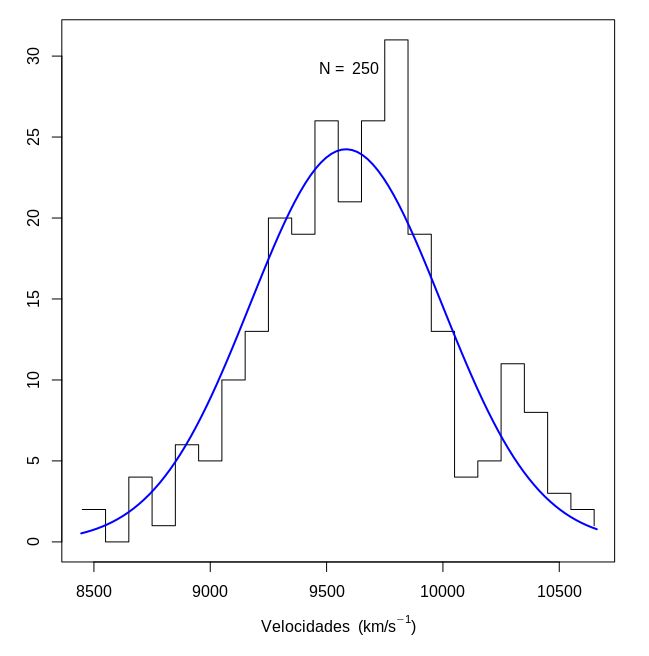
\includegraphics[width=0.3\textwidth]{04-figuras/distVel}
	\fonte{Autor}
	\label{fig1}
\end{figure}

O processo de formação de aglomerados de galáxias ainda não atingiu o seu fim. Enquanto regiões centrais estão em equilíbrio dinâmico, as regiões periféricas (externas) acumulam matéria na forma de galáxias ou grupos de galáxias de modo contínuo. Comumente o entorno dos aglomerados de galáxias é constituído de grupos de galáxias que podem ser absorvidos pelo aglomerado principal ao longo do tempo, ocasionando o aumento de sua massa (Rembold, 2011). Estudos sobre a distribuição de velocidades de galáxias em aglomerados indicam que a mesma possui distribuição Não Rejeita, vide Figura \ref{fig1}, ou muito bem ajustada por uma gaussiana somente na região virializada do sistema (região mais interna do sistema) (Yahil \& Vidal 1977), podendo existir sinais de múltiplos modos normais na região mais externa (Ribeiro, Lopes \& Trevisan 2011), comprovando a presença de componentes de um sistema em processo de evolução pelo acréscimo de matéria ao seu entorno. Esse acréscimo de matéria, na forma de galáxias ou grupo de galáxias.  Isto sugere que a formação de aglomerados de galáxias é um processo contínuo que decorre de fusões sucessivas e encontros gravitacionais de maiores e menores proporções (Nascimento et al., 2016).



\section{Distribuição de Velocidades ao longo do Aglomerado}
A velocidade de uma galáxia contida em um aglomerado, em uma dada posição, não pode ser maior que a velocidade de escape do sistema, caso isto aconteça a galáxia não pertenceria mais ao aglomerado. A velocidade de escape e a distância ao centro do aglomerado são grandezas inversamente proporcionais, ou seja, a velocidade de escape decresce com o aumento da distância ao centro do aglomerado, portanto é mais fácil o escape de uma galáxia que está na região periférica (de Oliveira e Viegas, 2004).

Para que o aglomerado exista como unidade dinâmica é preciso uma redução na amplitude da distribuição de velocidades das galáxias à medida que haja um afastamento da região central. O grande problema dessa propriedade é o efeito de projeção. As galáxias que estão com distâncias distintas do centro do aglomerado podem parecer ao observador com mesma distância em consequência da observação apenas das posições projetadas no plano do céu (de Oliveira e Viegas, 2004).

Na Figura \ref{fig2} vemos a distribuição de velocidades do aglomerado em função da distância da galáxia ao centro do aglomerado, onde o estreitamento da distribuição de velocidades define uma espécie de "corneta" que pode ser utilizada para definir os membros de um aglomerado, sendo removidas as galáxias que estejam significativamente acima ou abaixo da "corneta".

\begin{figure}[!htb]
	\centering
	\caption{Distribuição de velocidades em função da distância ao centro do Aglomerado.}
	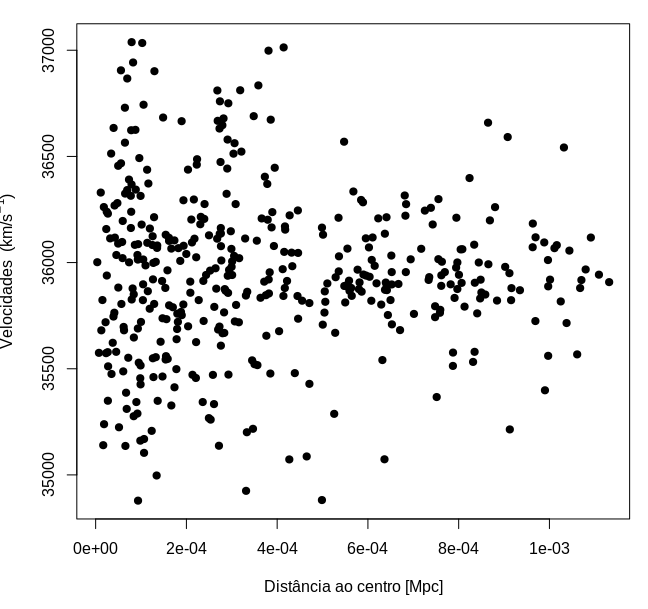
\includegraphics[width=0.3\textwidth]{04-figuras/distCenter}
	\fonte{Autor}
	\label{fig2}
\end{figure}

\chapter{Rotação de Aglomerados}

O conhecimento do estado dinâmico de aglomerados de galáxias pode propiciar restrições importantes em cenários cosmológicos, como a determinação da massa total do aglomerado e uma estimativa da quantidade de matéria escura no Universo. A possibilidade da existência de aglomerados em rotação tem sido discutida por muitos autores (por exemplo, veja os estudos de Hwang \& Lee 2007; Manaloupoulos \& Plionis 2016). 

Para detecção de indícios de rotação, Hwang \& Lee (2007) utilizaram dados espectroscópicos do \textit{Sloan Digital Sky Survey} \footnote{Considerado o mais ambicioso mapeamento astronômico que já foi feito. Com este mapeamento, os astrônomos podem observar os padrões de grande escala das galáxias: filamentos e vazios em grandes regiões angulares do Universo.}(SDSS) e \textit{Two-Degree-Field Galaxy Redshift Survey} (2dF-GRS). A rotação de aglomerados foi modelada como a rotação de galáxias membro e a rotação do gás intra-aglomerado. Eles levantaram inicialmente a hipótese de que a rotação se origina através de fusões de aglomerados. Um aspecto importante do método empregado por Hwang \& Lee (2007) é que os aglomerados com rotação devem exibir divisão espacial entre galáxias com velocidades maiores e menores que a velocidade média do aglomerado além de apresentar um pico no mapa de densidade. Nesta pesquisa de Hwang \& Lee (2007) foram detectados seis sistemas com rotação, em um total de dozes aglomerados (Abell 0954, Abell 1139, Abell 1399, Abell 2162, Abell 2169, and Abell 2366). Constatou-se ainda que estes aglomerados estão em equilíbrio dinâmico e não sofreram fusão recente, não dando suporte, portanto, à hipótese de interações como causadoras da rotação. 

Kalinkov et al. (2008) tentaram obter o gradiente máximo no campo de velocidades de Abell 2107 e determinaram que a direção do coeficiente de correlação linear máximo definiria o eixo maior do aglomerado e o eixo menor seria o de rotação. Foram utilizadas subamostras de galáxias membro, ordenadas de acordo a distância ao centro do aglomerado para definir o grau de rotação do sistema. Esse mesmo aglomerado foi estudado por Oegerle et al. (1992) e foram encontrados indícios de rotação. Materne et al. (1983) apontaram a dificuldade em diferenciar um aglomerado rotativo de dois que se sobrepõem, pelo motivo de estar se fundindo ou se afastando. Porém, o aglomerado  Abell 2107 não consiste de dois aglomerados sobrepostos, em consequência do pico estreito representado em seu histograma de velocidades. O indicador mais forte que definiu a rotação foi o ângulo de posição do eixo com o gradiente máximo no campo de velocidades quase coincidindo com o ângulo de posição do eixo com o maior alongamento.  Nesse estudo o período de rotação foi calculado em uma volta a cada $2.4\times10^9$ anos e houve uma correção no valor da massa para $2.8\times10^{14}~{M_\odot}$  (a massa inicial era de $3.2\times10^{14}~{M_\odot}$, sem levar em conta a rotação). 

Baseado no estudo da distribuição de velocidades das galáxias membro, Tovmassian (2015)  detectou sinais de rotação em 17 de uma amostra de 65 aglomerados (26\%). O método analisa o número de galáxias com velocidades mais baixas e mais altas que a velocidade média do aglomerado em diferentes partes do aglomerado. O método teve mais êxito em aglomerados planos, com $f=a/b > 1.8$ (a e b semieixos - maior e menor – da distribuição de galáxias do aglomerado). 
Para estes, a taxa de detecção de rotação foi mais alta (7 dos 18 aglomerados planos, 39\%).  Esse resultado suporta a opinião de que os aglomerados foram originalmente formados a partir das enormes nuvens de gás primordiais e preservaram a rotação das nuvens primordiais, a menos que sofram fusões com outros aglomerados e grupos de galáxias. 

Já na tese de Manolopoulou (2014) é realizado um estudo de um novo algoritmo para dedução de rotação usando a velocidade radial projetada\footnote{É a velocidade de um objeto na direção da linha de visada, isto é, a velocidade com que o objeto se aproxima ou se afasta do observador.}. Inicialmente os testes foram realizados em aglomerados gerados em simulações de Monte Carlo para confirmar se o método fornecia indicações robustas de rotação. Em seguida, aplicado em amostras de aglomerados de Abell. Através do teste de Kolmogorov-Smirnov, decidiu-se quanto a sua rotação significativa ou não, seu centro rotacional, orientação do eixo de rotação, amplitude de velocidade rotacional e, finalmente, o sentido de rotação no sentido horário ou anti-horário no plano do céu. Foram encontrados 23 aglomerados possivelmente rotativos dentro de 1.5 Mpc ou a uma distância de 2.5 Mpc do centro do aglomerado, do total de 45 da amostra.

\chapter{Ferramentas Estatísticas Utilizadas}
\section{Teste de Hipótese}
A análise estatística objetiva, especialmente, fazer inferência sobre uma população a partir da observação de uma amostra. Os testes de hipótese representam uma forma de inferência estatística. A hipótese é uma afirmação sobre parâmetros populacionais que devem ser analisadas para verificar sua veracidade. É importante ressaltar que a verdade ou não nunca pode ser determinada, a menos que toda a população seja observada, situação impraticável na maioria das vezes, justificado pelo uso do teste estatístico.  

A princípio é necessário estabelecer como verdadeira a \textbf{hipótese nula}, denotada por \textbf{$H_0$}. Já a \textbf{hipótese alternativa ($H_1$)}, contrapõe a hipótese nula, ou seja, $H_0$ deverá ser rejeitada. É necessário estabelecer um critério auxiliar para decidir a rejeição ou não de $H_0$ para um teste estatístico. Esse valor, determinado pelo pesquisador antes da análise de dados ou até mesmo na coleta de dados, cenário ideal, é denominado \textbf{nível alfa ($\alpha$) ou nível de significância}. Comumente é utilizado como critério de rejeição uma probabilidade de 5\%. De acordo com Cramer e Howitt (2004), 

\begin{citacao}
O nível em que a hipótese nula é rejeitada é geralmente definido como 5 ou menos vezes fora de 100. Isso significa que tal diferença ou relacionamento é provável que ocorra por acaso 5 ou menos vezes de 100. Este nível é geralmente descrito como proporção 0.05 e às vezes como a porcentagem 5\%. O nível de probabilidade de 0.05 foi historicamente uma escolha arbitrária, mas tem sido aceitável como uma escolha razoável na maioria das circunstâncias. Se houver um motivo para variar este nível, é aceitável fazer então. Então, em circunstâncias em que pode haver consequências adversas muito graves se a decisão errada foi feita sobre a hipótese, então o nível de significância poderia ser mais rigoroso em, digamos, 1\% (Cramer and Howitt, 2004: 151). 
\end{citacao}

Na realização de testes de hipóteses é possível que erros sejam cometidos, como mostrado no quadro \ref{qua:hipotese}. \textbf{Erro do tipo I}, denotado por \textbf{erro $\alpha$}, a rejeição de $H_0$ quando ela é verdadeira. Contrapondo, a não-rejeição de $H_0$ quando esta é falsa é denominada \textbf{erro do tipo II} e representado por \textbf{$\beta$}.  Esse tipo de teste permite concluir se deve aceitar ou rejeitar a hipótese nula, porém não é possível quantificar o quão provável é o resultado de ocorrer ao acaso. Apoiado por isto, é definido a potência de um teste estatístico $1-\beta$ como a probabilidade de rejeitar $H_0$ quando de fato é falsa. Claramente, o teste ideal é aquele em que os valores de $\alpha$ e $\beta$ são mínimos. Porém, o valor de $\alpha$ é inversamente relacionado com o valor de $\beta$, sendo impossível minimizá-los simultaneamente. Geralmente, é fixado o nível de significância $\alpha$ e escolhido a região de rejeição que minimiza $\beta$, ou seja, que maximize a potência do teste. 


\begin{quadro}[!htb]
	\centering
	\caption{Tipos de erros em testes de hipótese.\label{qua:hipotese}}
	\begin{tabular}{|l|l|l|ll}
		\cline{1-3}
\multicolumn{1}{|c|}{\multirow{2}{*}{\textbf{Decisão Estatística}}} & \multicolumn{2}{l|}{\textbf{Natureza (estado verdadeiro ou desconhecido)}} &  &  \\ \cline{2-3}
\multicolumn{1}{|c|}{} & \multicolumn{1}{c|}{\textbf{$H_0$ verdadeira}} & \multicolumn{1}{c|}{\textbf{$H_1$ falsa}} &  &  \\ \cline{1-3}
\textbf{Aceitar $H_0$} & acerto & Erro tipo II ( \ensuremath{\beta}) &  &  \\ \cline{1-3}
\textbf{Rejeitar $H_0$} & Erro tipo I ( \ensuremath{alpha}) & acerto &  &  \\ \cline{1-3}
	\end{tabular}
	\fonte{\citeonline{}}
\end{quadro}

O menor nível de significância pode ser definido utilizando o \textbf{valor-p} ou \textbf{\textit{“p-value”}}. No teste de hipótese esse valor é comparado ao nível de significância \ensuremath{alpha} determinado no início objetivando a tomada de decisão de aceitar ou rejeitar $H_0$. Se o valor-p calculado do teste for igual ou maior que \ensuremath{alpha}, a $H_0$ é aceita. Ou seja, a hipótese nula é consistente com os resultados da amostra. Porém, se o valor-p for menor que \ensuremath{alpha}, a hipótese nula é rejeitada, a hipótese alternativa, nesse caso, é então aceita como verdadeira.

\section{Teste de Normalidade}
Uma variável aleatória, seja idade de um grupo de pessoas ou ocorrência de um determinado desfecho, pode admitir uma distribuição de frequências da população, contendo diversas formas encontradas na literatura estatística. O intuito desses modelos é caracterizar o comportamento de um determinado evento em função da frequência de sua ocorrência. Se as variáveis forem contínuas, o evento será um intervalo de valores. Portanto, as distribuições de frequências são efetivamente distribuições de probabilidade, em que para um evento teremos associado uma probabilidade de ocorrência (T2). 

A inspeção visual pode ser utilizada para avaliação da normalidade. A distribuição de frequência, como exemplo um histograma, relaciona valores observados à sua frequência e pode além de pressupor uma distribuição normal, identifica \textit{insights} sobre lacunas nos dados e outliers. O histograma é composto por barras justapostas em que no eixo horizontal contém a variável de interesse dividida em classes e no eixo vertical a sua correspondente frequência (T2). Para distribuições do tipo normal ou Gaussiana, o histograma constitui formato de sino (Figura 3b).

Entretanto, a simples constatação por meio de gráficos é subjetiva e não satisfatória, pois depende de uma interpretação visual além de não ser confiável no caso multivariado e especificamente nas situações de muitas variáveis. Desta forma, para inferir sobre a normalidade é necessário utilizar como complemento testes estatísticos (T1).  Como exemplo, podemos citar: o teste de aderência qui-quadrado; Kolmogorov-Smirnov; Lilliefors e Shapiro-Wilk. 

Estes testes possuem estatísticas de teste e critérios de decisão diferentes, porém compartilham da hipótese avaliada: a hipótese de nulidade ($H_0$) especifica que a variável aleatória adere à distribuição normal, sem a necessidade de definir a média ou variância da distribuição. Já a hipótese alternativa ($H_1$), opõe a hipótese nula (T2). 

O resultado que interessa após executar um determinado teste é o seu valor-p ou nível descritivo do teste, referente à probabilidade de que a estatística do teste (como variável aleatória) tenha valor extremo em comparação ao valor observado (estatística) quando a hipótese nula é verdadeira. Sendo o valor-p menor que o nível de significância, logo a hipótese nula é rejeitada. Ou seja, o valor-p representa o menor nível de significância que pode assumir para então rejeitar a hipótese nula. Logo, há significância estatística quando o valor-p é menor que o nível de significância estabelecido (FLÁVIO – ESTUDO DA DISTRIBUIÇÃO).  

\section{Testes utilizados}
\subsection{Teste de Cramer-von Mises}
Em estatística, o teste de Cramér (conhecido também como phi de Cramer - $\varphi$c) é uma medida de associação entre duas variáveis nominais dado o intervalo de 0 a 1, indicando que um valor mais alto possui forte associação. Fundamentado no teste estatístico do qui-quadrado de Pearson, foi publicado em 1946 por Harald Cramér. A medida é definida como

\begin{equation}
\ V = \sqrt{\frac{{\chi_{obt}}^2}{N.m}}
\label{eq:eq1}
\end{equation}
	
	onde $\chi^2$ é o valor obtido do teste estatístico
	
	N é o tamanho da amostra e 
    
    m = o menor de (r - 1) ou (c – 1), sendo r o número de linhas e c o número de colunas.

Para entender melhor a utilidade do teste de Cramer é fundamental compreender as formas como os testes estatísticos divergem das medidas de associação para variáveis categóricas. O teste qui-quadrado ($\chi^2$) fornece um teste estatístico de associação entre duas variáveis categóricas (nominais) de uma população única. Ele determina se a associação entre as variáveis é significativa, utilizando como hipótese nula ($H_0$) que as duas variáveis não são dependentes uma da outra e como hipótese alternativa ($H_1$) é que existe alguma associação entre duas variáveis.

O teste de Cramer é considerado um dos favoritos entre as medidas baseadas no qui-quadrado. Geralmente, quando o seu cálculo resulta no valor máximo 1 é que exista um forte relacionamento entre duas variáveis. No cálculo de Cramer é levado em consideração as dimensões da tabela, ou seja, diferentes dimensões podem ser comparadas significativamente.

\subsection{Teste de Hotelling}

Um dos mais conhecidos testes de hipóteses multivariados foi proposto por Harold Hotelling em 1947, o teste de $T^2$, compara vetores de médias populacionais. Baseado na generalização da estatística \textit{t de Student}, foi o primeiro a levar em consideração a correlação das variáveis na formulação da estatística do teste.

Sendo \textbf{\textit{X}} um vetor aleatório com uma dada dimensão, \textbf{\textit{$\mu$}} o vetor de médias e \textbf{\textit{$\sigma$}} a matriz de covariância. Para \textbf{\textit{X}}, sendo uma distribuição Não Rejeita multivariada e com tamanho de amostra aleatória \textbf{\textit{n}}, a estatística de $T^2$ é dada por
\begin{equation}
\ T^2 = n(\overline{X} - \mu_0) \sum_{pxp}^{-1} {(\overline{X} - \mu_0)}
\label{eq:eq2}
\end{equation}

com

\begin{equation}
 H_0 : \mu = \mu_0 \\
 H_1 : \mu \neq \mu_0
\label{eq:eq3}
\end{equation}

A equação \ref{eq:eq2} tem distribuição qui-quadrado com \textit{p} graus de liberdade. Definindo um nível de significância $\alpha$, com $0 < \alpha < 1$, para valores de $T^2$  maiores ou iguais ao valor crítico ${\chi^2_{a,p,c}}$ dado por $P[{\chi_p}^2 \geq {\chi^2_{a,p,c}}]$,  a hipótese nula será rejeitada.   

Sendo a matriz desconhecida, a estatística de $T^2$ é dada por

\begin{equation}
T^2 = n(\overline{X} -\mu_0) S^{-1}(\overline{X} - \mu_0)
\label{eq:eq4}
\end{equation}

que sob a hipótese nula, tem uma distribuição proporcional a uma distribuição F, ou seja, o valor crítico do teste a um nível de significância $\alpha$, com $0 < \alpha < 1$, é

\begin{equation}
F_c = \frac{p(n-1)}{n-p} F_{1-\alpha, p, n - p}
\label{eq:eq5}
\end{equation}

onde $F_{1-\alpha, p, n - p}$ é a probabilidade acumulada igual a (1 - $\alpha$) da distribuição de F com p
n-p é igual a graus de liberdade.

Sendo S a matriz de covariâncias amostrais (\textit{pxp}), um estimado não viciado de $\sum_{pxp}$, dado por
\begin{equation}
\begin{bmatrix}
S^{2}_{1} & S_{12} & ... & S_{1p} \\ 
 & S^{2}_{2} & ... & S_{2p} \\ 
 &  & \ddots  & \vdots  \\ 
 &  &  & S^{2}_{p}
\end{bmatrix}
 \label{eq:eq6}
\end{equation}

em que os elementos da diagonal principal de S são as variâncias definidos por
\begin{equation}
S^2_j = \frac{1}{m-1} \sum_{k=1}^m (x_{jk} - \overline{X}_j),    j = 1, 2, ..., 3 
\label{eq:eq7}
\end{equation}

e os elementos fora da diagonal principal são as covariâncias conforme

\begin{equation}
S_{jh} = \frac{1}{m-1} \sum_{k=1}^m (x_{jk} - \overline{X}_j)(x_{hk} - \overline{X}_h) 
\label{eq:eq8}
\end{equation}

onde $x_{jk}$ e $x_{hk}$ representam os valores amostrais das variáveis $X_j$ e $X_h$.	% Elementos da dissertação/tese
	% %
% 
%

\chapter{Citações e Referências}\label{referencias}
Neste capítulo, assim como nos anteriores procuramos inserir muitas citações bibliográficas a fim de familiarizar os autores com as diferentes maneiras de fazê-las e nesse sentido a classe é bastante versátil. Os principais itens de bibliografia citados são livros, artigos em conferências,
artigos em jornais e páginas Web. A bibliografia deve seguir as normas da ABNT e também da UESC.

Citações são trechos transcritos ou informações retiradas das publicações consultadas para a realização do trabalho.
As citações são utilizadas no texto com o propósito de esclarecer, completar, embasar ou corroborar as ideias do autor.

Todas as publicações consultadas e efetivamente utilizadas (através de citações) devem ser listadas, obrigatoriamente, nas referências bibliográficas, de forma a preservar os direitos autorais e intelectuais, conforme consta nas normas da ABNT e da UESC.

A bibliografia é feita no padrão {\ttfamily bibtex}. As referências são colocadas em um arquivo separado. Nesse caso o arquivo  {\ttfamily refbase}. Fizemos questão de colocar uma referência de cada formato de fontes mais popular: livros, jornais, mídias na internet, etc.

Os elementos de cada item bibliográfico que devem constar na bibliografia são apresentados a seguir.

Para livros, o formato da bibliografia no arquivo fonte é o seguinte:

\begin{verbatim}
@Book{linked,
   author = {A. L. Barabasi},
   title = {Linked: The New Science of Networks},
   publisher = {Perseus Publishing},
   year = {2002},
}
\end{verbatim}

A citação deste livro se faz da seguinte forma \verb#\cite{linked}# e o resultado fica assim \cite{linked}.
Para os artigos em {\textit jornais}, veja por exemplo \cite{carvalho:2001},
descrito da seguinte forma no arquivo {\ttfamily .bib}:

\begin{verbatim}
@Article{carvalho:2001,
  Title                    = {Inteligência competitiva numa visão de futuro},
  Author                   = {Cláudia Carvalho and José Fajardo and Joaquim Cruz},
  Journal                  = {DataGramaZero - Revista da Ciência da Informação},
  Year                     = {2001},
  Number                   = {3},
  Pages                    = {12--16},
  Volume                   = {2},

  Mounth                   = {junho},
  Subtitle                 = {proposta metodológica}
}
\end{verbatim}


Veja também duas citações juntas \cite{Zimmermann,GomideandPed} e como citar
endereços Web \cite{irl:06}.


\section{Citação indiretas ou livres}\label{ciação direta}

As citações indiretas são feitas com base no comando \verb|\citeonline{label}|, onde \verb|label| corresponde a um nome dado para chamar a referência no texto. O comando \verb|\citeonline{maturana:2003}| gera a seguinte citação indireta: \citeonline{maturana:2003} defende um princípio de lógica...

Além disso, \citeonline{teste:2014} argumenta que \ldots\mbox{ } Observe o detalhe do termo \textit{et al}.
que deve ser utilizado quando o trabalho citado possui mais de três autores. Este é o padrão do estilo {\ttfamily abntex2}.
Caso por algum motivo não deseje abreviar o nome dos demais autores através do termo \textit{et al.}, deve-se incluir a opção {\ttfamily abnt-no-etal-label}.

Para evitar uma interrupção na sequência do texto, o que poderia, eventualmente, prejudicar a leitura, pode-se indicar a fonte entre parênteses imediatamente após a citação indireta. Porém, neste caso específico, o nome do autor deve vir em caixa alta, seguido do ano da publicação, como no exemplo a seguir.

A física, então, constituiu-se como a prova mínima da efetividade do método científico para descobrir as verdades do universo \cite{teste:2014,maturana:2003}. Essa citação foi obtida com o comando \verb|\cite{teste:2014,maturana:2003}|


\section{Citações diretas ou literais}\label{citacoesdiretas}

Há várias maneiras de se fazer uma citação literal, como mostra os exemplos abaixo.

As citações longas (mais de 3 linhas) devem usar um parágrafo específico para ela, na forma de um texto recuado (4 cm da margem esquerda), com tamanho de letra menor do aquela utilizada no texto e espaçamento simples entre as linhas, seguido dos sobrenomes dos autores em caixa alta (separados por ponto e vírgula), ano de publicação e número da página.

As citações diretas são obtidas com o comando \verb|\cite{label}|. Veja o exemplo abaixo onde usamos o ambiente citação e o comando \verb|\cite[p.~28]{morinmoigne:2000}| para citar o autor.

\begin{citacao}
Desse modo, opera-se uma ruptura decisiva entre a reflexividade filosófica, isto 	é a possibilidade do sujeito de pensar e de refletir, e a objetividade científica.
Encontramo-nos num ponto em que o conhecimento científico está sem consciência.
Sem consciência moral, sem consciência reflexiva e também subjetiva.
Cada vez mais o desenvolvimento extraordinário do conhecimento científico vai tornar menos praticável a própria possibilidade de reflexão do sujeito sobre a sua pesquisa \cite[p.~28]{morinmoigne:2000}.
\end{citacao}

A sintaxe do ambiente citação utilizado acima é a seguinte:
\begin{verbatim}
    \begin{citacao}
        <citacao>
    \end{citacao}
\end{verbatim}

Opcionalmente, pode-se referenciar os autores no corpo de texto (neste caso seus nomes devem vir em minúsculas), e em seguida colocar a citação literal, em um novo parágrafo recuado. Nesse caso após a citação literal não mais aparece o nome dos autores, visto que já se encontra no texto.
Veja o exemplo seguinte.

\citeonline[p.~33]{morinmoigne:2000}, ao fazerem as suas críticas à ciência, explicitam uma ideia coletiva:

\begin{citacao}
Mas o curioso é que o conhecimento científico que descobriu os meios realmente extraordinários para, por exemplo, ver aquilo que se passa no nosso sol, para tentar conceber a estrutura das estrelas extremamente distantes, e até mesmo para tentar pesar o universo, o que é algo de extrema utilidade, o conhecimento científico que multiplicou seus meios de observação e de concepção do universo, dos objetos, está completamente cego, se quiser considerar-se apenas a si próprio!
\end{citacao}

As citações curtas (menos de 3 linhas) devem ser inseridas diretamente no texto (entre aspas), seguida do nome do autor (em caixa alta), ano e página, como no exemplo a seguir.

Então significa apenas que ``assumo que não posso fazer referência a entidades independentes de mim para construir meu explicar'' \cite[p.~35]{maturana:2003}.

\section{Resumo dos comandos para  referências }\label{referenciasUtilizadas}

Apresentamos abaixo exemplos de referências já citadas no texto com seus comandos.

\begin{itemize}
	\item \citeonline{maturana:2003}\\ \verb|\citeonline{maturana:2003}|
	\item \citeonline{teste:2014}\\ \verb|\citeonline{teste:2014}|
	\item \cite[p.~28]{morinmoigne:2000}\\ \verb|\cite[p.~28]{morinmoigne:2000}|
	\item \citeonline[p.~33]{morinmoigne:2000}\\ \verb|\citeonline[p.~33]{morinmoigne:2000}|
	\item \cite[p.~35]{maturana:2003}\\ \verb|\cite[p.~35]{maturana:2003}|
	\item \citeonline[p.~35]{maturana:2003}\\ \verb|\citeonline[p.~35]{maturana:2003}|
	\item \cite{teste:2014,maturana:2003}\\ \verb|\cite{teste:2014,maturana:2003}|
\end{itemize}
	% citações e refeerencias
	% 
\chapter{Figuras, Tabelas e outros elementos}\label{chap:fundamentacaoTeorica}
A seguir ilustra-se a forma de incluir figuras, tabelas, equações, siglas e símbolos no documento, obtendo indexação automática em suas respectivas listas.
A numeração sequencial de figuras, tabelas e equações ocorre de modo automático.
Referências cruzadas são obtidas através dos comandos \verb#\label{}# e \verb#\ref{}#.
Por exemplo, estou me referindo agora a introdução que corresponde ao  capítulo \ref{chap:introducao}. Todos os comandos utilizados para gerar os elementos desse texto estão nos respectivos arquivos dos capítulos. Não os colocaremos aqui para que o texto não fique demasiadamente extenso e não ficarmos repetitivos.

\section{Figuras}
\label{sec:figuras}

Abaixo é apresentado um exemplo de figura. A  figura \ref{fig:brasaouesc} aparece automaticamente na lista de figuras. Para uso avançado de imagens no LATEX, recomenda-se a consulta de literatura especializada.

\begin{figure}[!htb]
	\centering
	\caption{Brasão da UESC}
	
\includegraphics[width=0.3\textwidth]{./04-figuras/brasaouesc}
	\fonte{\citeonline{teste:2014}}
	\label{fig:brasaouesc}
\end{figure}

\subsection{Figuras lado a lado}\label{figladoalado}
Para colocar figuras lado a lado com legendas diferentes utilizamos o pacote {\ttfamily subfigure}, declarado no preâmbulo. Porém o pacote abntex, no qual é baseado a classe, é incompatível com o pacote {\ttfamily subfigure}. Ao tentar usá-lo a compilação apresenta erros de incompatibilidade. 

Para contornar essa situação fiz algumas alterações necessárias no pacote e o renomeei como {\ttfamily subfigureppmgc}. Assim, caso você queira utilizar no seu texto figuras lado a lado com legendas diferentes, deve utilizar essa nova versão do  pacote, o qual se encontra na pasta {\ttfamily pacotes}. A classe já está configurada para utilizá-lo automaticamente.

Caso as figuras que fiquem lado a lado  utilizem apenas uma legenda não há necessidade do pacote, basta chamá-las normalmente no ambiente {\ttfamily figure}.

Abaixo segue um exemplo de como fica a utilização do pacote inserindo figuras lado a lado, com legendas diferentes.\\

\begin{figure}[!htb]
 \caption{Imagens comparando o estado do rio Cachoeira a dez anos atrás e atualmente} \label{fig:estadorc}
\subfigure[ Imagem do rio Cachoeira a dez anos atras\label{fig:rc-adezanos}]{
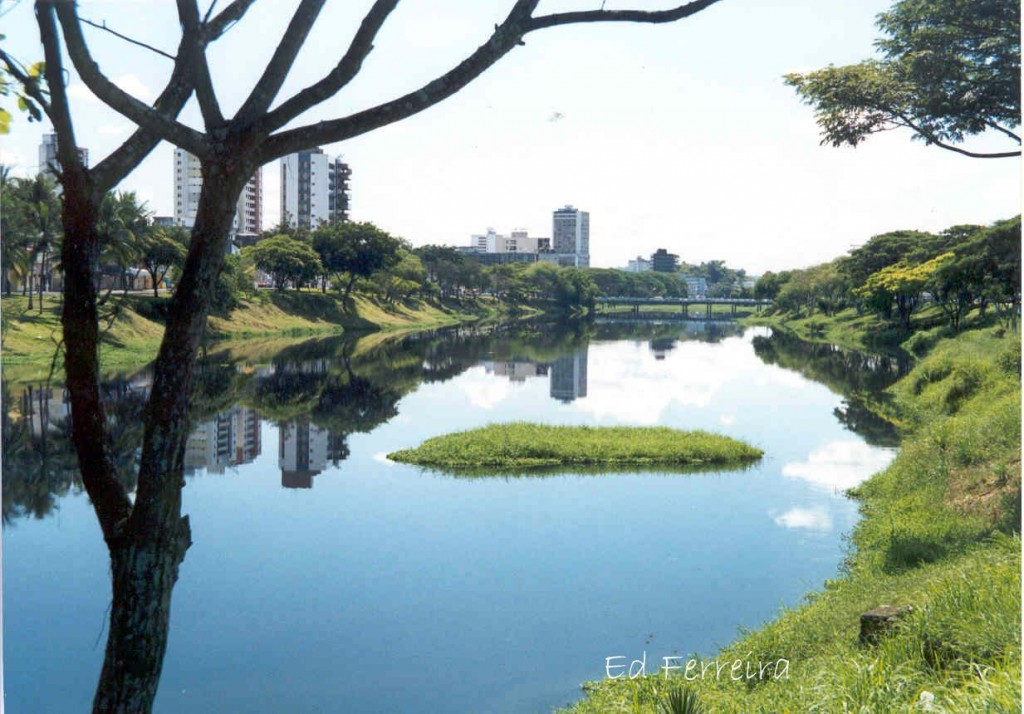
\includegraphics[width=7cm,height=6cm]{04-figuras/rc-adezanos}}
\subfigure[Imagem atual do rio Cachoeira\label{fig:rc-atualmente}]{
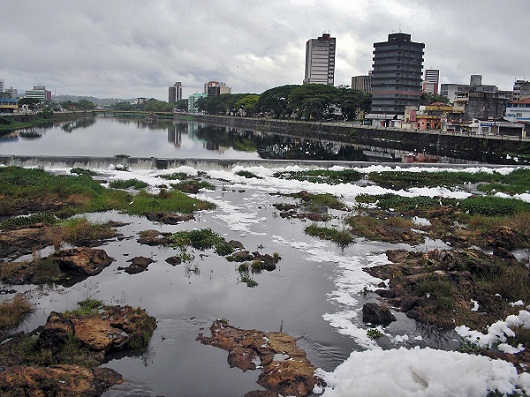
\includegraphics[width=7cm,height=6cm]{04-figuras/rc-atualmente}}
\fonte{Pimenta Blog.BR, no endereço em $<$http://www.pimenta.blog.br/$>$}
\end{figure}
\section{Quadros e Tabelas}
\label{sec:tabelas}

Também é apresentado o exemplo do quadro \ref{qua:comparabd} e da tabela \ref{tab:correlacao}, que aparece automaticamente na lista de quadros e tabelas.
Informações sobre a construção de tabelas no LATEX podem ser encontradas na literatura especializada e diversas apostilas encontradas livremente na internet  \cite{Lamport1986,Buerger1989,reginaldo,camargo}.

\begin{quadro}[!htb]
	\centering
	\caption{Hierarquia de restrições das questões.\label{qua:comparabd}}
	\begin{tabular}{|p{7cm}|p{7cm}|}
		\hline
		\textbf{BD Relacionais} & \textbf{BD Orientados a Objetos} \\
		\hline
		Os dados são passivos, ou seja, certas operações limitadas podem ser automaticamente acionadas quando os dados são usados. Os dados são ativos, ou seja, as solicitações fazem com que os objetos executem seus métodos. & Os processos que usam dados mudam constantemente. \\
		\hline
	\end{tabular}
	\fonte{\citeonline{teste:2014}}
\end{quadro}

\newpage
Exemplos de tabelas:

\begin{table}[!htb]
	\centering
	\caption[Correlação de valores x e y]{Exemplo de uma tabela mostrando a correlação entre x e y.\label{tab:correlacao}}
	\begin{tabular}{cc}
		\hline
			x & y \\
		\hline
			1 & 2 \\
			3 & 4 \\
			5 & 6 \\
			7 & 8 \\
		\hline
	\end{tabular}
	\fonte{Autoria própria.}
\end{table}


\begin{table}[!htb]
	\centering
	\caption[Resultado dos testes]{Resultado dos testes.\label{tab:testes}}
	\begin{tabular}{rrrrr}
		\toprule
			& Valores 1 & Valores 2 & Valores 3 & Valores 4 \\
		\midrule
			Caso 1 & 0,86 & 0,77 & 0,81 & 163 \\
			Caso 2 & 0,19 & 0,74 & 0,25 & 180 \\
			Caso 3 & 1,00 & 1,00 & 1,00 & 170 \\
		\bottomrule
	\end{tabular}
\end{table}


\section{Equações}
\label{sec:equacoes}

A transformada de Laplace é dada na equação \ref{eq:laplace}, enquanto a equação \ref{eq:dft} apresenta a formulação da transformada discreta de Fourier bidimensional\footnote{Deve-se reparar na formatação esteticamente perfeita destas equações.}.

\begin{equation}
	X(s) = \int\limits_{t = -\infty}^{\infty} x(t) \, \text{e}^{-st} \, dt
	\label{eq:laplace}
\end{equation}

\begin{equation}
	F(u, v) = \sum_{m = 0}^{M - 1} \sum_{n = 0}^{N - 1} f(m, n) \exp \left[ -j 2 \pi \left( \frac{u m}{M} + \frac{v n}{N} \right) \right]
	\label{eq:dft}
\end{equation}


		% tabelas e figuras
	% %
% Documento: Conclusão
\chapter{Conclusão}\label{chap:conclusao}
Neste trabalho apresentamos um método de detecção de rotação em aglomerados de galáxias desenvolvido em R. Nosso objetivo foi investigar um dos aspectos menos estudados a respeito de aglomerados, que é a possibilidade de que eles tenham algum grau de rotação. Não levar em consideração a rotação de aglomerados pode gerar um erro nas suas estimativas de massa. O entendimento, controle e redução deste tipo de erro são de grande importância para a astrofísica extragaláctica. 

Utilizamos os catálogos \textbf{selec20}, composto por 20 aglomerados; \textbf{NoSocs}, com 183 aglomerados, sendo que 25 aglomerados continham um total inferior a 20 objetos, sendo inviável o cálculo de detecção; \textbf{III} que geramos duas amostras I e II de aglomerados com grau de rotação e sem rotação, respectivamente. 

Além da aplicação do nosso método nos catálogos, implementamos o método de Hwang \& Lee que utiliza a relação sinoidal para o cálculo do ângulo do eixo de rotação $\theta_o$ e a velocidade de rotação $v_{rot}$. Os resultados foram comparados e como conclusão temos que:

\begin{itemize}
   \item \textbf{Para o catálogo I (selec20)}: o nosso método detectou 14 aglomerados com evidência de rotação. Já o método de Hwang \& Lee detectou um grau de rotação para todos os aglomerados. 
   \item \textbf{Para o catálogo II (NoSocs)}: com total de 158 aglomerados, aproximadamente 39.87\%, ou seja, 63 dos aglomerados, dectectaram rotação. Diferente do nosso método, o de Hwang \& Lee considerou os 183 aglomerados e detectou rotação em 97.81\% deles.   
   \item \textbf{Para o catálogo I (selec20)}: para este catálogo simulamos duas amostras I e II com 200 aglomerados em cada um deles. Na amostra I todos os aglomerados tinham um grau de rotação. Já na amostra II, todos os aglomerados eram sem rotação. No nosso método, para a amostra I, detectamos rotação em todos os aglomerados, enquanto o método de Hwang \& Lee apenas 96.5\% dos casos. Para a amostra II, o nosso método detectou rotação em 13.5\% dos aglomerados e o de Hwang \& Lee um total de 96.5\%.
 \end{itemize}     

 Como desconhecemos as propriedades dinâmicas dos catálogos I e II utilizamos o método de Monte Carlo para simular amostras de aglomerados com rotação e sem rotação. Nesse cenário, nosso método obteve resultados mais seguros.


\section{Trabalhos Futuros}
\label{sec:trabalhosFuturos}

Como perspectivas, temos que uma possível continuação deste trabalho é realizar a correção no cálculo da massa através da fórmula \ref{eq:massa}. 

\begin{equation}
\omega^2 R = {GM}/{R},
\label{eq:massa}
\end{equation}
onde $\omega$ é a velocidade rotacional, R é o raio, M a massa e G é a constante gravitacional.		% Conclusão

%========================================================================================================================
% elementos pós textuais
 	\postextual
 	\bibliography{./03-elementos-pos-textuais/refbase}
% %

 	\include{./03-elementos-pos-textuais/glossario}	% Glossário
 	% %
% Documento: Apêndice
%

\begin{apendicesenv}
\partapendices

\chapter{Nome do apêndice}
\label{chap:apendicex}

Inserir seu texto aqui...

\chapter{Nome do apêndice}
\label{chap:apendicey}

Inserir seu texto aqui...

\end{apendicesenv}		% Apêndices
 	%
% Documento: Anexos
%

\begin{anexosenv}
\partanexos

\chapter{Resultados Catálogo selec20}
\label{chap:anexoselec20}

Com a aplicação do nosso método nos 20 aglomerados do catálogo selec20 obtivemos os seguintes resultados, dado o histograma de velocidade, o eixo principal e o perfil de rotação apenas para os aglomerados que apresentaram rotação significativa.  

\begin{figure}[H] %h or !htbp
\vspace{-2pt}
\centering
\subfloat{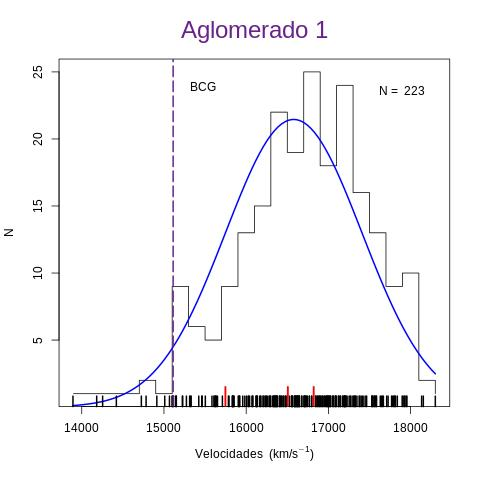
\includegraphics[scale=.23]{04-figuras/selec20/dist01}}
\subfloat{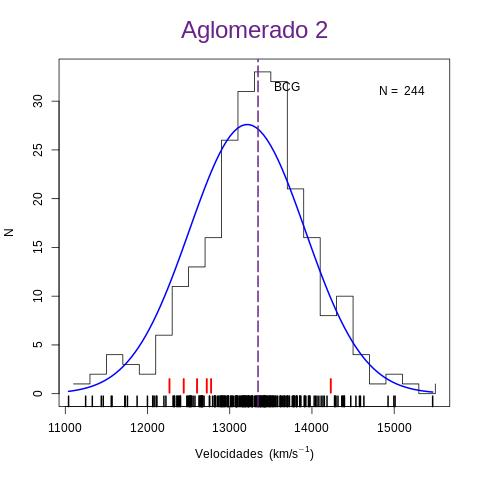
\includegraphics[scale=.23]{04-figuras/selec20/dist02}}
\subfloat{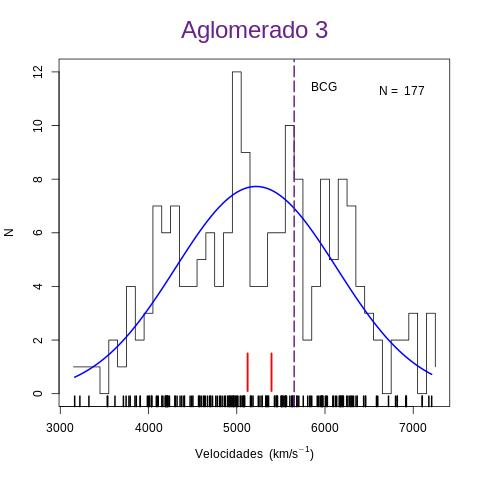
\includegraphics[scale=.23]{04-figuras/selec20/dist03}}
\subfloat{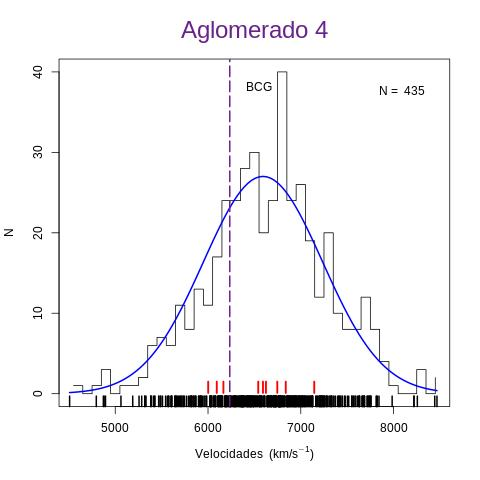
\includegraphics[scale=.23]{04-figuras/selec20/dist04}}\hfill
\subfloat{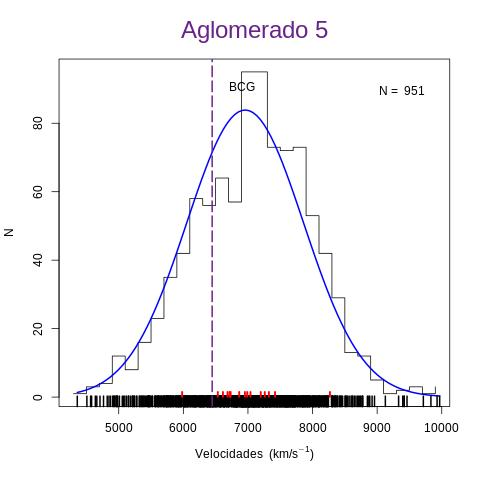
\includegraphics[scale=.23]{04-figuras/selec20/dist05}}
\subfloat{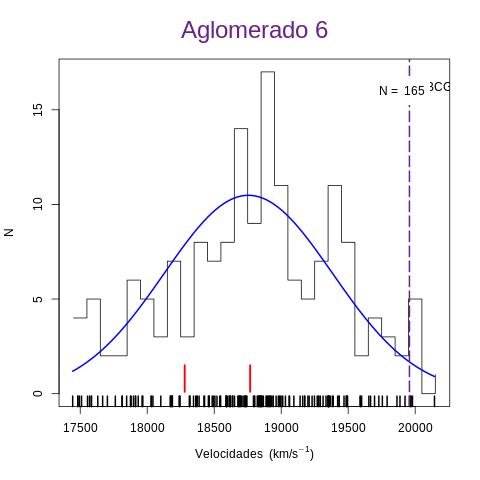
\includegraphics[scale=.23]{04-figuras/selec20/dist06}}
\subfloat{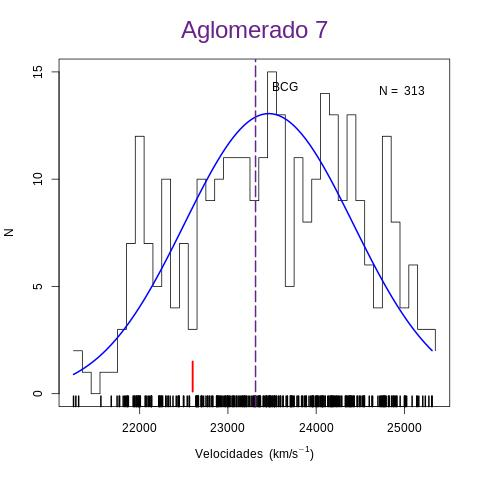
\includegraphics[scale=.23]{04-figuras/selec20/dist07}}
\subfloat{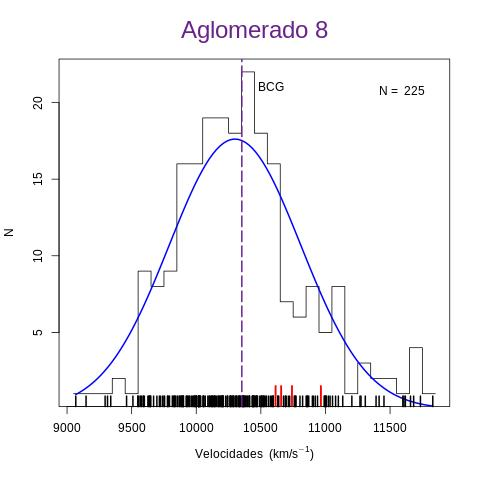
\includegraphics[scale=.23]{04-figuras/selec20/dist08}}\hfill
\subfloat{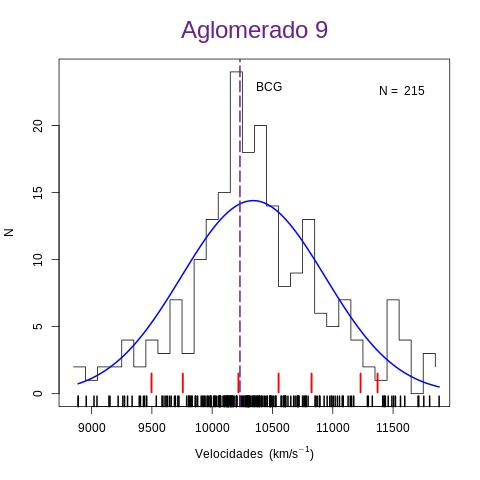
\includegraphics[scale=.23]{04-figuras/selec20/dist09}}
\subfloat{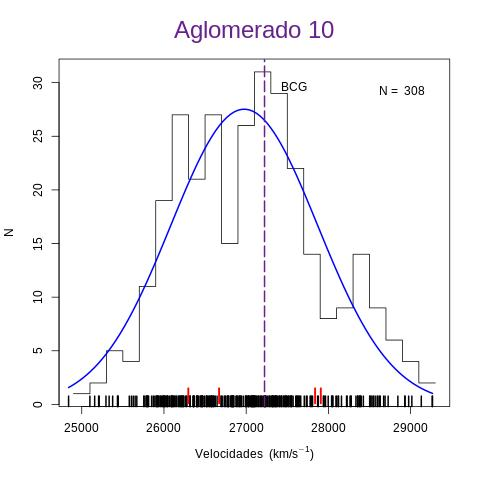
\includegraphics[scale=.23]{04-figuras/selec20/dist10}}
\subfloat{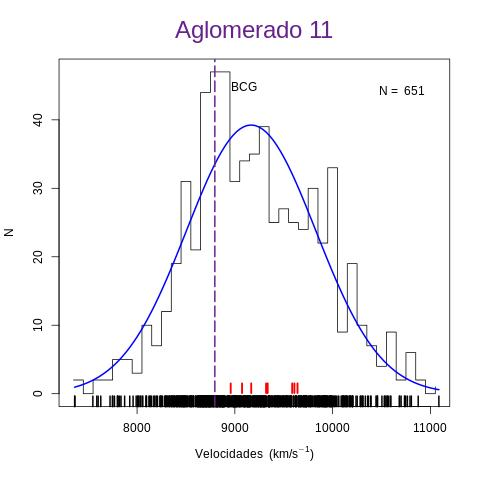
\includegraphics[scale=.23]{04-figuras/selec20/dist11}}
\subfloat{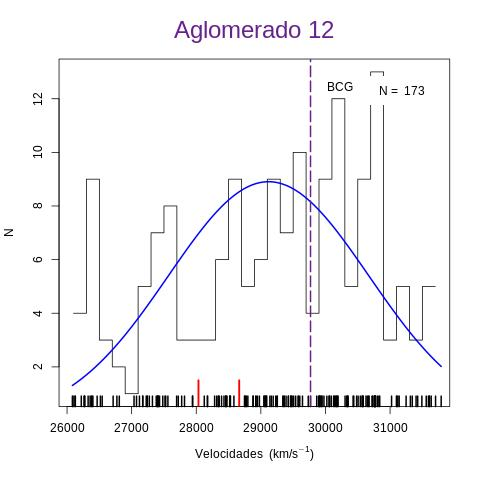
\includegraphics[scale=.23]{04-figuras/selec20/dist12}}\hfill
\subfloat{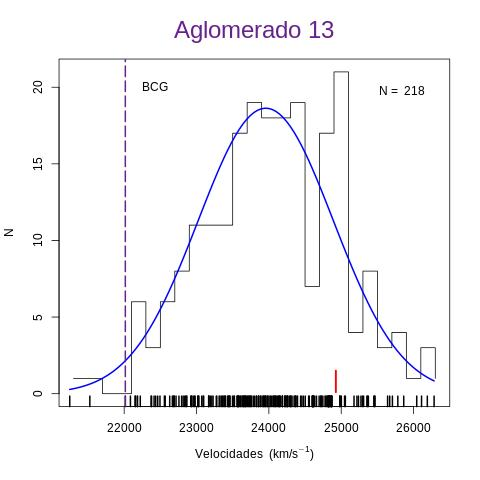
\includegraphics[scale=.23]{04-figuras/selec20/dist13}}
\subfloat{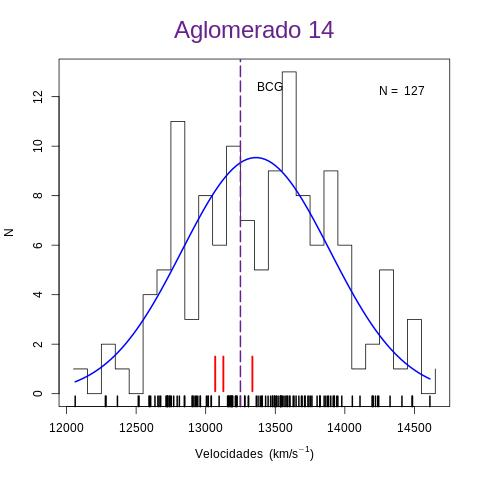
\includegraphics[scale=.23]{04-figuras/selec20/dist14}}
\subfloat{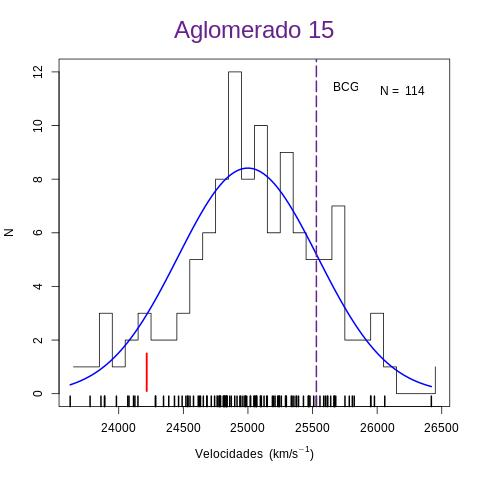
\includegraphics[scale=.23]{04-figuras/selec20/dist15}}
\subfloat{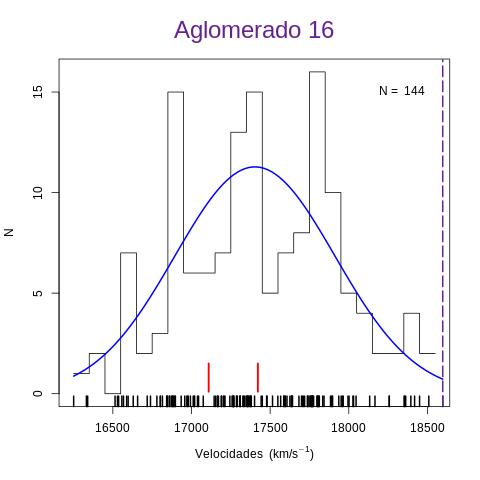
\includegraphics[scale=.23]{04-figuras/selec20/dist16}}\hfill
\subfloat{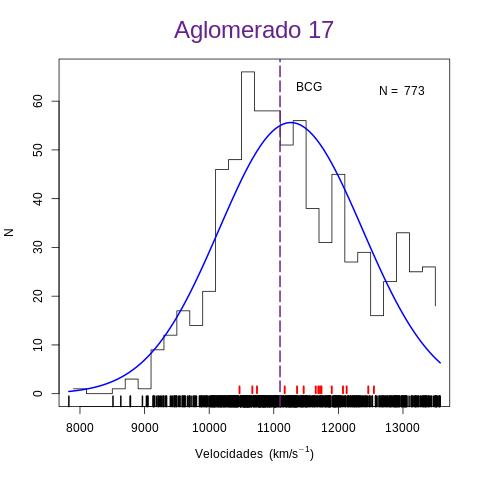
\includegraphics[scale=.23]{04-figuras/selec20/dist17}}
\subfloat{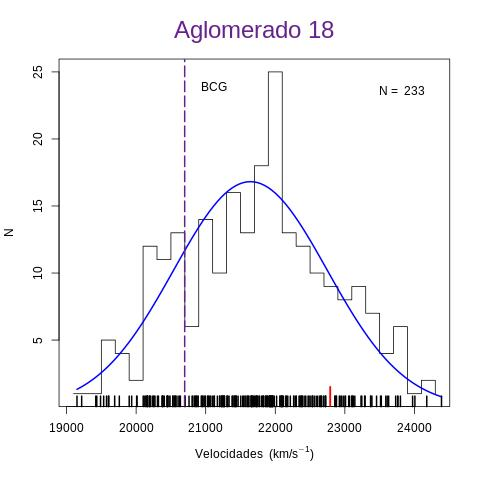
\includegraphics[scale=.23]{04-figuras/selec20/dist18}}
\subfloat{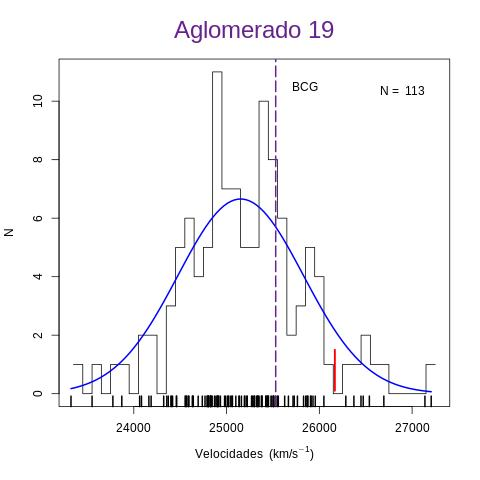
\includegraphics[scale=.23]{04-figuras/selec20/dist19}}
\subfloat{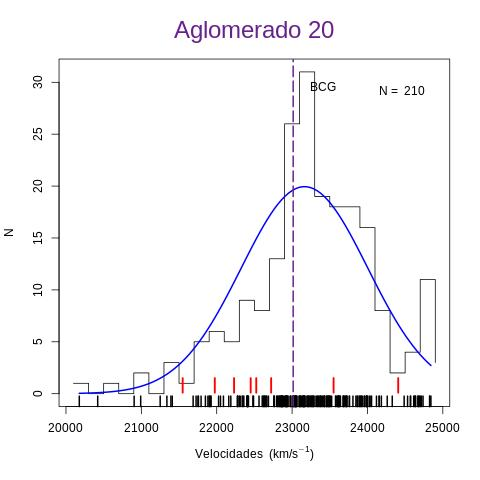
\includegraphics[scale=.23]{04-figuras/selec20/dist20}}
\caption{Histograma Distribuição de Velocidade e Análise de Gaps.}
\label{fig:fig4}%
\end{figure}


\begin{figure}[H] %h or !htbp
\vspace{-2pt}
\begin{center}
\subfloat{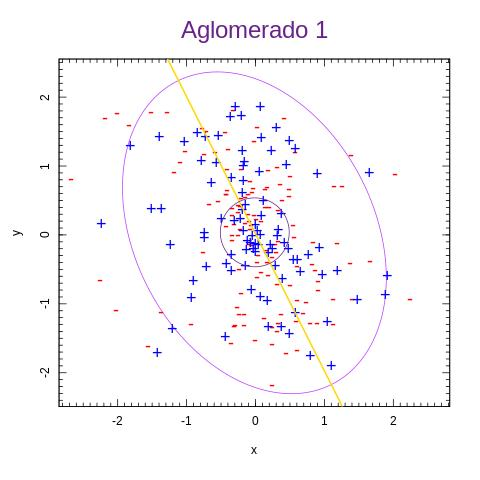
\includegraphics[scale=.23]{04-figuras/selec20/eixo01}}
\subfloat{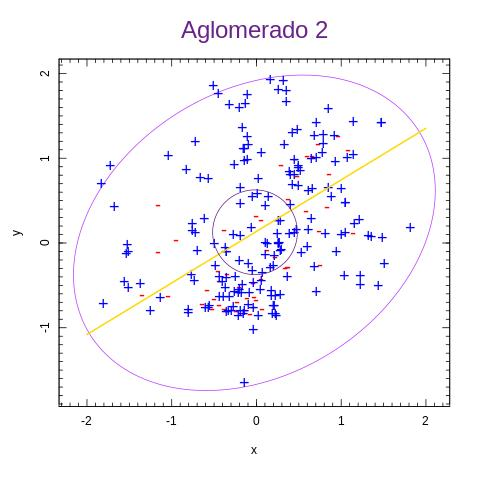
\includegraphics[scale=.23]{04-figuras/selec20/eixo02}}
\subfloat{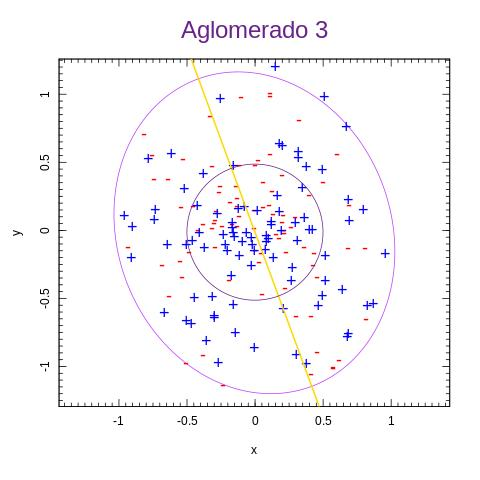
\includegraphics[scale=.23]{04-figuras/selec20/eixo03}}
\subfloat{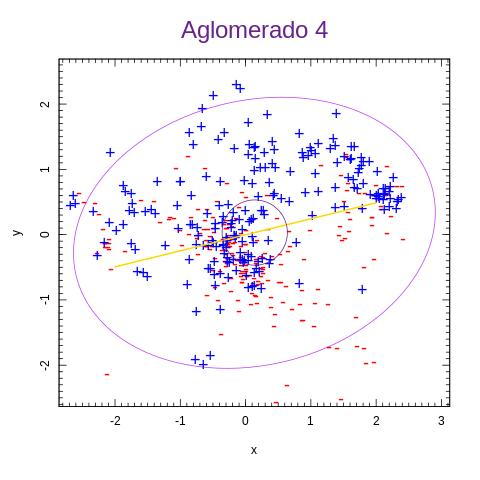
\includegraphics[scale=.23]{04-figuras/selec20/eixo04}}\hfill
\subfloat{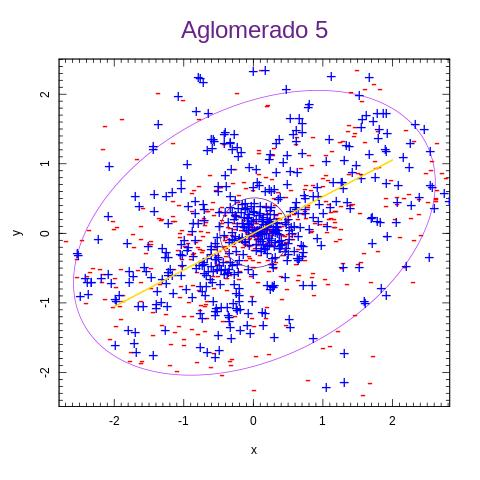
\includegraphics[scale=.23 ]{04-figuras/selec20/eixo05}}
\subfloat{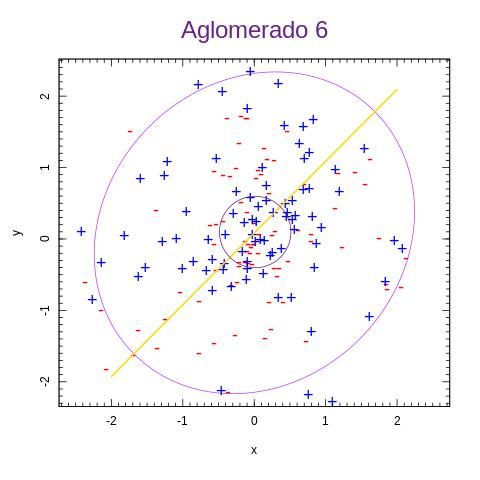
\includegraphics[scale=.23 ]{04-figuras/selec20/eixo06}}
\subfloat{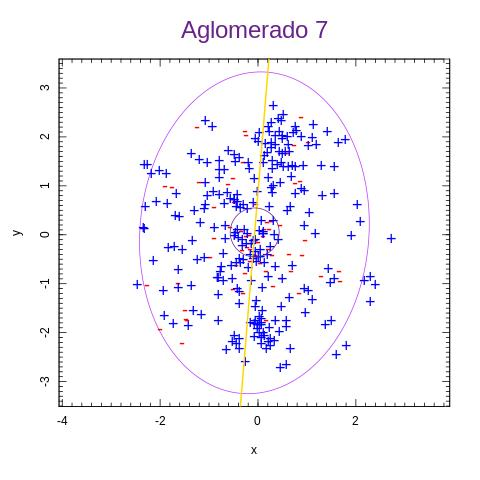
\includegraphics[scale=.23 ]{04-figuras/selec20/eixo07}}
\subfloat{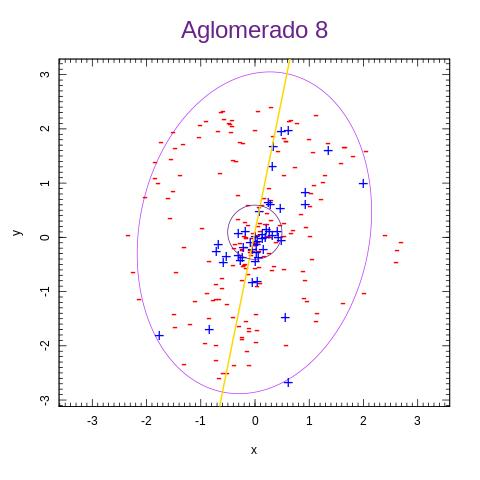
\includegraphics[scale=.23 ]{04-figuras/selec20/eixo08}}\hfill
\subfloat{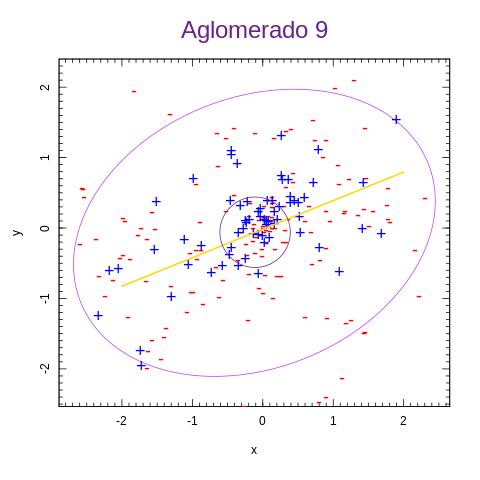
\includegraphics[scale=.23 ]{04-figuras/selec20/eixo09}}
\subfloat{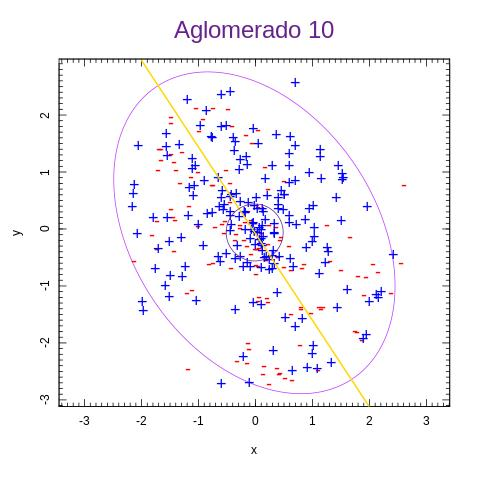
\includegraphics[scale=.23 ]{04-figuras/selec20/eixo10}}
\subfloat{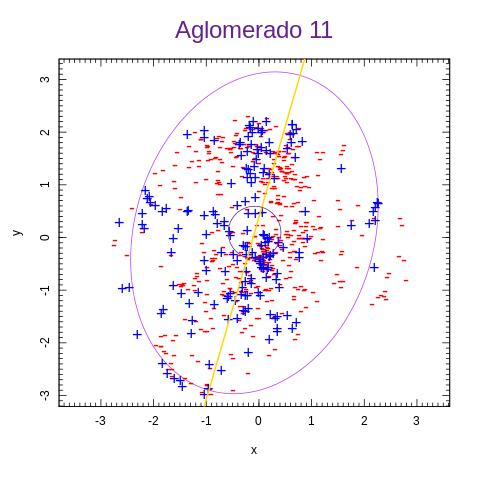
\includegraphics[scale=.23 ]{04-figuras/selec20/eixo11}}
\subfloat{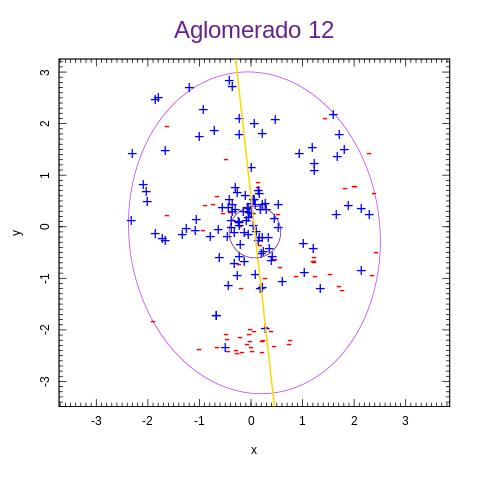
\includegraphics[scale=.23 ]{04-figuras/selec20/eixo12}}\hfill
\subfloat{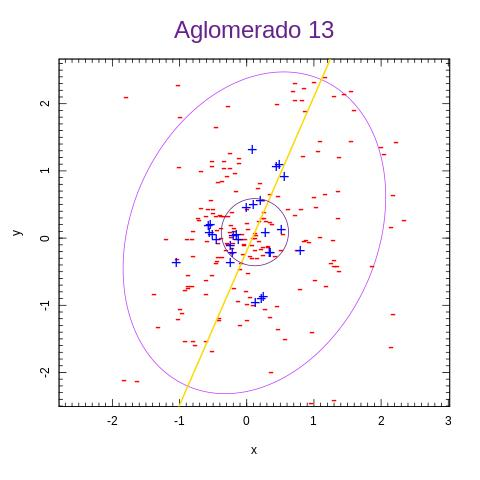
\includegraphics[scale=.23 ]{04-figuras/selec20/eixo13}}
\subfloat{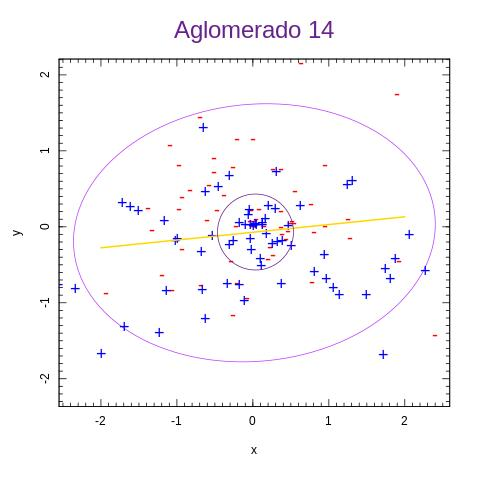
\includegraphics[scale=.23 ]{04-figuras/selec20/eixo14}}
\subfloat{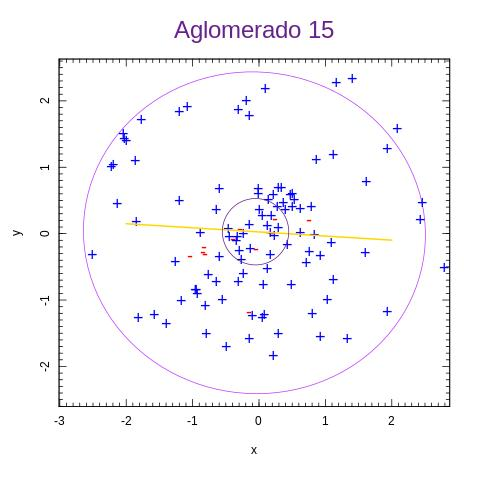
\includegraphics[scale=.23 ]{04-figuras/selec20/eixo15}}
\subfloat{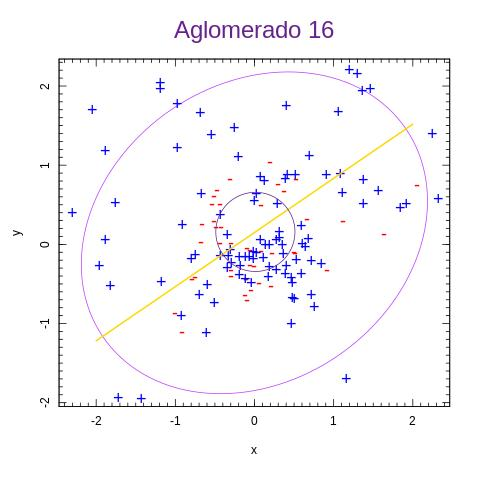
\includegraphics[scale=.23 ]{04-figuras/selec20/eixo16}}\hfill
\subfloat{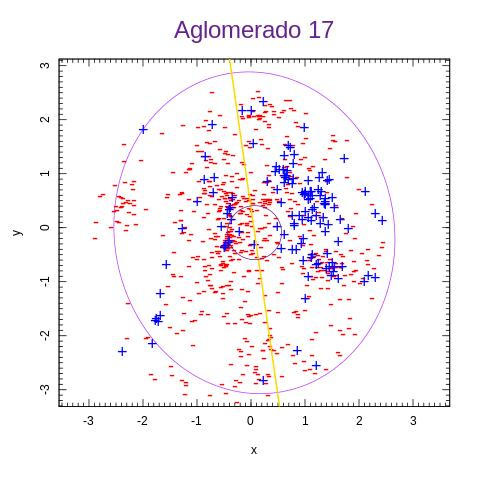
\includegraphics[scale=.23 ]{04-figuras/selec20/eixo17}}
\subfloat{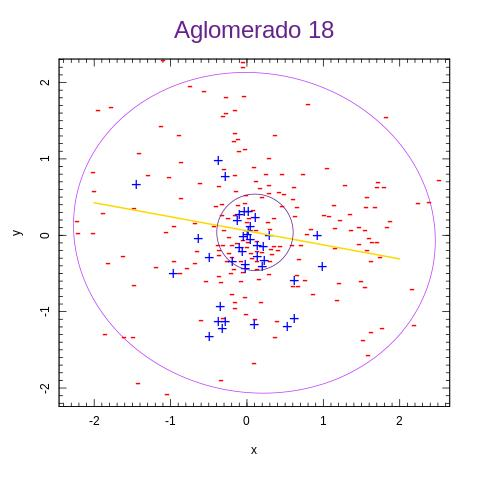
\includegraphics[scale=.23 ]{04-figuras/selec20/eixo18}}
\subfloat{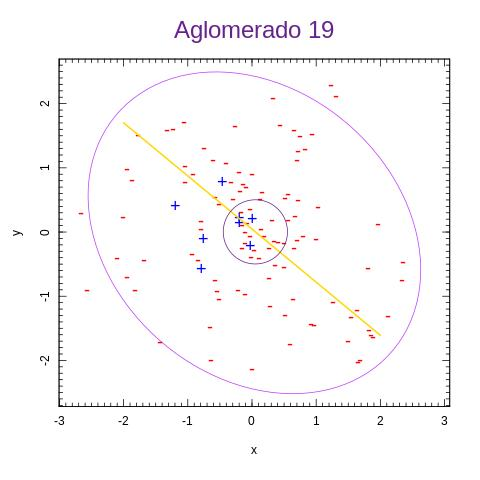
\includegraphics[scale=.23 ]{04-figuras/selec20/eixo19}}
\subfloat{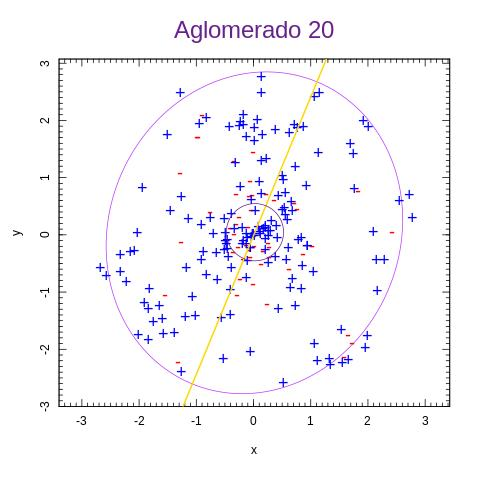
\includegraphics[scale=.23 ]{04-figuras/selec20/eixo20}}
\caption{Ajuste da elipse e eixo principal da distribuição projetada no plano do céu.}
\label{fig5}%
\end{center}
\end{figure}


\begin{figure}[H] %h or !htbp
\vspace{-2pt}
\begin{center}
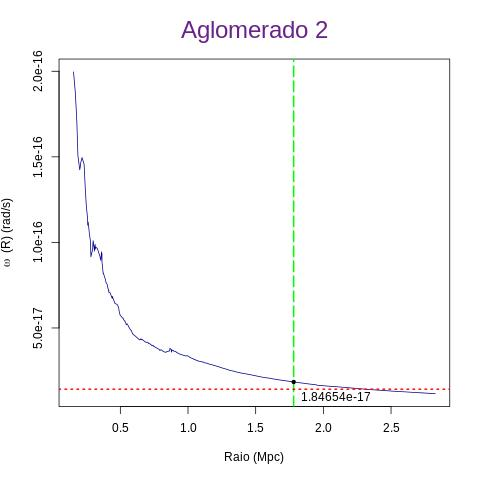
\includegraphics[scale=.3]{04-figuras/selec20/perfil02}%
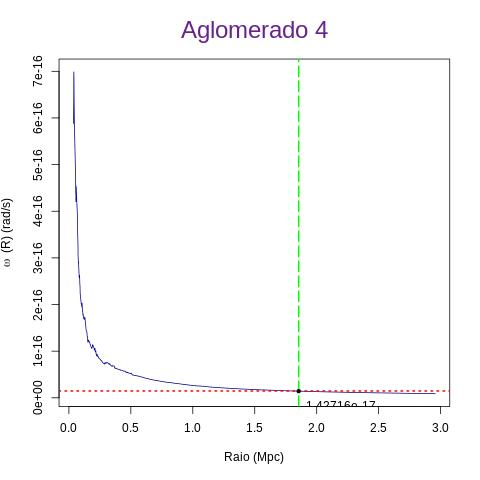
\includegraphics[scale=.3]{04-figuras/selec20/perfil04}
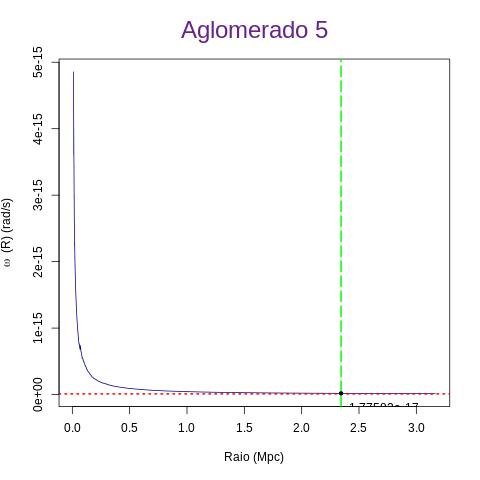
\includegraphics[scale=.3]{04-figuras/selec20/perfil05}
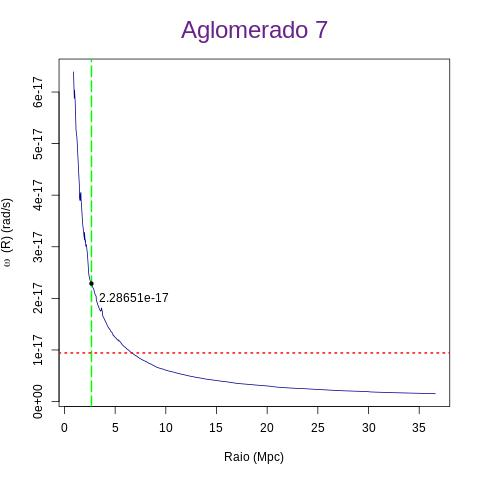
\includegraphics[scale=.3]{04-figuras/selec20/perfil07}\hfill
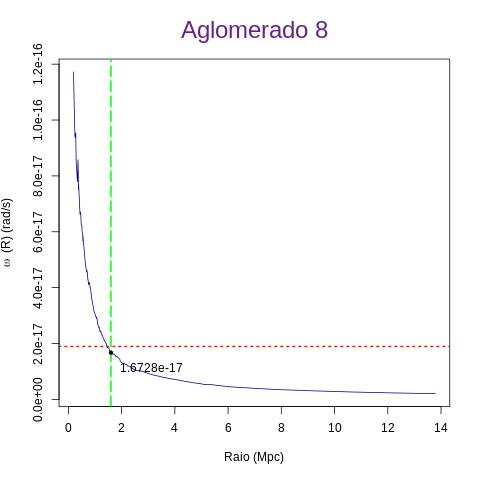
\includegraphics[scale=.3]{04-figuras/selec20/perfil08}
\includegraphics[scale=.3]{04-figuras/selec20/perfil09}
\includegraphics[scale=.3]{04-figuras/selec20/perfil10}
\includegraphics[scale=.3]{04-figuras/selec20/perfil11}\hfill
\includegraphics[scale=.3]{04-figuras/selec20/perfil12}
\includegraphics[scale=.3]{04-figuras/selec20/perfil14}
\includegraphics[scale=.3]{04-figuras/selec20/perfil15}
\includegraphics[scale=.3]{04-figuras/selec20/perfil16}\hfill
\includegraphics[scale=.3]{04-figuras/selec20/perfil17}
\includegraphics[scale=.3]{04-figuras/selec20/perfil18}
\caption{Perfil da velocidade de rotação.}
\label{fig6}%
\end{center}
\end{figure}

\chapter{Resultados Catálogo NoSOCS}
\label{chap:anexonosocs}
Os resultados obtidos na aplicação do nosso método para o catálogo NoSOCS são os seguintes, dado o histograma de velocidade, o eixo principal, a tabela comparativa dos testes utilizados (Cramer e Hotelling) e o perfil de rotação apenas para os aglomerados que apresentaram rotação significativa.

\begin{figure}[H] %h or !htbp
\vspace{-2pt}
\centering
\subfloat{\includegraphics[scale=.23]{04-figuras/nosocs/dist00339}}
\subfloat{\includegraphics[scale=.23]{04-figuras/nosocs/dist00996}}
\subfloat{\includegraphics[scale=.23]{04-figuras/nosocs/dist01052}}
\subfloat{\includegraphics[scale=.23]{04-figuras/nosocs/dist01189}}\hfill
\subfloat{\includegraphics[scale=.23]{04-figuras/nosocs/dist01238}}
\subfloat{\includegraphics[scale=.23]{04-figuras/nosocs/dist01264}}
\subfloat{\includegraphics[scale=.23]{04-figuras/nosocs/dist01347}}
\subfloat{\includegraphics[scale=.23]{04-figuras/nosocs/dist01831}}\hfill
\subfloat{\includegraphics[scale=.23]{04-figuras/nosocs/dist01836}}
\subfloat{\includegraphics[scale=.23]{04-figuras/nosocs/dist01877}}
\subfloat{\includegraphics[scale=.23]{04-figuras/nosocs/dist01933}}
\subfloat{\includegraphics[scale=.23]{04-figuras/nosocs/dist02104}}\hfill
\subfloat{\includegraphics[scale=.23]{04-figuras/nosocs/dist02137}}
\subfloat{\includegraphics[scale=.23]{04-figuras/nosocs/dist02298}}
\subfloat{\includegraphics[scale=.23]{04-figuras/nosocs/dist02301}}
\subfloat{\includegraphics[scale=.23]{04-figuras/nosocs/dist02433}}\hfill
\subfloat{\includegraphics[scale=.23]{04-figuras/nosocs/dist02440}}
\subfloat{\includegraphics[scale=.23]{04-figuras/nosocs/dist02447}}
\subfloat{\includegraphics[scale=.23]{04-figuras/nosocs/dist02469}}
\subfloat{\includegraphics[scale=.23]{04-figuras/nosocs/dist02490}}\hfill
\subfloat{\includegraphics[scale=.23]{04-figuras/nosocs/dist02752}}
\subfloat{\includegraphics[scale=.23]{04-figuras/nosocs/dist02899}}
\subfloat{\includegraphics[scale=.23]{04-figuras/nosocs/dist03112}}
\subfloat{\includegraphics[scale=.23]{04-figuras/nosocs/dist03176}}
\caption{Histograma Distribuição de Velocidade e Análise de Gaps.}
\label{fig:fig4}%
\end{figure}

\begin{figure}[H] %h or !htbp
\vspace{-2pt}
\centering
\subfloat{\includegraphics[scale=.23]{04-figuras/nosocs/dist03229}}
\subfloat{\includegraphics[scale=.23]{04-figuras/nosocs/dist03459}}
\subfloat{\includegraphics[scale=.23]{04-figuras/nosocs/dist03565}}
\subfloat{\includegraphics[scale=.23]{04-figuras/nosocs/dist03691}}\hfill
\subfloat{\includegraphics[scale=.23]{04-figuras/nosocs/dist03742}}
\subfloat{\includegraphics[scale=.23]{04-figuras/nosocs/dist03898}}
\subfloat{\includegraphics[scale=.23]{04-figuras/nosocs/dist03907}}
\subfloat{\includegraphics[scale=.23]{04-figuras/nosocs/dist03915}}\hfill
\subfloat{\includegraphics[scale=.23]{04-figuras/nosocs/dist03975}}
\subfloat{\includegraphics[scale=.23]{04-figuras/nosocs/dist04023}}
\subfloat{\includegraphics[scale=.23]{04-figuras/nosocs/dist04048}}
\subfloat{\includegraphics[scale=.23]{04-figuras/nosocs/dist04100}}\hfill
\subfloat{\includegraphics[scale=.23]{04-figuras/nosocs/dist04376}}
\subfloat{\includegraphics[scale=.23]{04-figuras/nosocs/dist04404}}
\subfloat{\includegraphics[scale=.23]{04-figuras/nosocs/dist04405}}
\subfloat{\includegraphics[scale=.23]{04-figuras/nosocs/dist04409}}\hfill
\subfloat{\includegraphics[scale=.23]{04-figuras/nosocs/dist04458}}
\subfloat{\includegraphics[scale=.23]{04-figuras/nosocs/dist04470}}
\subfloat{\includegraphics[scale=.23]{04-figuras/nosocs/dist04479}}
\subfloat{\includegraphics[scale=.23]{04-figuras/nosocs/dist04672}}\hfill
\subfloat{\includegraphics[scale=.23]{04-figuras/nosocs/dist04681}}
\subfloat{\includegraphics[scale=.23]{04-figuras/nosocs/dist04703}}
\subfloat{\includegraphics[scale=.23]{04-figuras/nosocs/dist04710}}
\subfloat{\includegraphics[scale=.23]{04-figuras/nosocs/dist05039}}
\caption{Histograma Distribuição de Velocidade e Análise de Gaps.}
\label{fig:fig4}%
\end{figure}

\begin{figure}[H] %h or !htbp
\vspace{-2pt}
\centering
\subfloat{\includegraphics[scale=.23]{04-figuras/nosocs/dist05206}}
\subfloat{\includegraphics[scale=.23]{04-figuras/nosocs/dist05325}}
\subfloat{\includegraphics[scale=.23]{04-figuras/nosocs/dist05359}}
\subfloat{\includegraphics[scale=.23]{04-figuras/nosocs/dist05447}}\hfill
\subfloat{\includegraphics[scale=.23]{04-figuras/nosocs/dist05535}}
\subfloat{\includegraphics[scale=.23]{04-figuras/nosocs/dist05717}}
\subfloat{\includegraphics[scale=.23]{04-figuras/nosocs/dist05859}}
\subfloat{\includegraphics[scale=.23]{04-figuras/nosocs/dist05908}}\hfill
\subfloat{\includegraphics[scale=.23]{04-figuras/nosocs/dist06070}}
\subfloat{\includegraphics[scale=.23]{04-figuras/nosocs/dist06173}}
\subfloat{\includegraphics[scale=.23]{04-figuras/nosocs/dist06175}}
\subfloat{\includegraphics[scale=.23]{04-figuras/nosocs/dist06184}}\hfill
\subfloat{\includegraphics[scale=.23]{04-figuras/nosocs/dist06207}}
\subfloat{\includegraphics[scale=.23]{04-figuras/nosocs/dist06233}}
\subfloat{\includegraphics[scale=.23]{04-figuras/nosocs/dist06256}}
\subfloat{\includegraphics[scale=.23]{04-figuras/nosocs/dist06261}}\hfill
\subfloat{\includegraphics[scale=.23]{04-figuras/nosocs/dist06264}}
\subfloat{\includegraphics[scale=.23]{04-figuras/nosocs/dist06286}}
\subfloat{\includegraphics[scale=.23]{04-figuras/nosocs/dist06392}}
\subfloat{\includegraphics[scale=.23]{04-figuras/nosocs/dist06447}}\hfill
\subfloat{\includegraphics[scale=.23]{04-figuras/nosocs/dist06475}}
\subfloat{\includegraphics[scale=.23]{04-figuras/nosocs/dist06506}}
\subfloat{\includegraphics[scale=.23]{04-figuras/nosocs/dist06508}}
\subfloat{\includegraphics[scale=.23]{04-figuras/nosocs/dist06547}}
\caption{Histograma Distribuição de Velocidade e Análise de Gaps.}
\label{fig:fig4}%
\end{figure}

\begin{figure}[H] %h or !htbp
\vspace{-2pt}
\centering
\subfloat{\includegraphics[scale=.23]{04-figuras/nosocs/dist06723}}
\subfloat{\includegraphics[scale=.23]{04-figuras/nosocs/dist06841}}
\subfloat{\includegraphics[scale=.23]{04-figuras/nosocs/dist06924}}
\subfloat{\includegraphics[scale=.23]{04-figuras/nosocs/dist07204}}\hfill
\subfloat{\includegraphics[scale=.23]{04-figuras/nosocs/dist07217}}
\subfloat{\includegraphics[scale=.23]{04-figuras/nosocs/dist07395}}
\subfloat{\includegraphics[scale=.23]{04-figuras/nosocs/dist07435}}
\subfloat{\includegraphics[scale=.23]{04-figuras/nosocs/dist07520}}\hfill
\subfloat{\includegraphics[scale=.23]{04-figuras/nosocs/dist07703}}
\subfloat{\includegraphics[scale=.23]{04-figuras/nosocs/dist07775}}
\subfloat{\includegraphics[scale=.23]{04-figuras/nosocs/dist07837}}
\subfloat{\includegraphics[scale=.23]{04-figuras/nosocs/dist07975}}\hfill
\subfloat{\includegraphics[scale=.23]{04-figuras/nosocs/dist08022}}
\subfloat{\includegraphics[scale=.23]{04-figuras/nosocs/dist08173}}
\subfloat{\includegraphics[scale=.23]{04-figuras/nosocs/dist08219}}
\subfloat{\includegraphics[scale=.23]{04-figuras/nosocs/dist08291}}\hfill
\subfloat{\includegraphics[scale=.23]{04-figuras/nosocs/dist08710}}
\subfloat{\includegraphics[scale=.23]{04-figuras/nosocs/dist08720}}
\subfloat{\includegraphics[scale=.23]{04-figuras/nosocs/dist08721}}
\subfloat{\includegraphics[scale=.23]{04-figuras/nosocs/dist08738}}\hfill
\subfloat{\includegraphics[scale=.23]{04-figuras/nosocs/dist08742}}
\subfloat{\includegraphics[scale=.23]{04-figuras/nosocs/dist08975}}
\subfloat{\includegraphics[scale=.23]{04-figuras/nosocs/dist09061}}
\subfloat{\includegraphics[scale=.23]{04-figuras/nosocs/dist09132}}
\caption{Histograma Distribuição de Velocidade e Análise de Gaps.}
\label{fig:fig4}%
\end{figure}

\begin{figure}[H] %h or !htbp
\vspace{-2pt}
\centering
\subfloat{\includegraphics[scale=.23]{04-figuras/nosocs/dist09148}}
\subfloat{\includegraphics[scale=.23]{04-figuras/nosocs/dist09153}}
\subfloat{\includegraphics[scale=.23]{04-figuras/nosocs/dist09157}}
\subfloat{\includegraphics[scale=.23]{04-figuras/nosocs/dist09162}}\hfill
\subfloat{\includegraphics[scale=.23]{04-figuras/nosocs/dist09176}}
\subfloat{\includegraphics[scale=.23]{04-figuras/nosocs/dist09177}}
\subfloat{\includegraphics[scale=.23]{04-figuras/nosocs/dist10001}}
\subfloat{\includegraphics[scale=.23]{04-figuras/nosocs/dist10004}}\hfill
\subfloat{\includegraphics[scale=.23]{04-figuras/nosocs/dist10006}}
\subfloat{\includegraphics[scale=.23]{04-figuras/nosocs/dist10008}}
\subfloat{\includegraphics[scale=.23]{04-figuras/nosocs/dist10009}}
\subfloat{\includegraphics[scale=.23]{04-figuras/nosocs/dist10010}}\hfill
\subfloat{\includegraphics[scale=.23]{04-figuras/nosocs/dist10013}}
\subfloat{\includegraphics[scale=.23]{04-figuras/nosocs/dist10014}}
\subfloat{\includegraphics[scale=.23]{04-figuras/nosocs/dist10015}}
\subfloat{\includegraphics[scale=.23]{04-figuras/nosocs/dist10016}}\hfill
\subfloat{\includegraphics[scale=.23]{04-figuras/nosocs/dist10017}}
\subfloat{\includegraphics[scale=.23]{04-figuras/nosocs/dist10018}}
\subfloat{\includegraphics[scale=.23]{04-figuras/nosocs/dist10019}}
\subfloat{\includegraphics[scale=.23]{04-figuras/nosocs/dist10020}}\hfill
\subfloat{\includegraphics[scale=.23]{04-figuras/nosocs/dist10021}}
\subfloat{\includegraphics[scale=.23]{04-figuras/nosocs/dist10022}}
\subfloat{\includegraphics[scale=.23]{04-figuras/nosocs/dist10023}}
\subfloat{\includegraphics[scale=.23]{04-figuras/nosocs/dist10024}}
\caption{Histograma Distribuição de Velocidade e Análise de Gaps.}
\label{fig:fig4}%
\end{figure}

\begin{figure}[H] %h or !htbp
\vspace{-2pt}
\centering
\subfloat{\includegraphics[scale=.23]{04-figuras/nosocs/dist10025}}
\subfloat{\includegraphics[scale=.23]{04-figuras/nosocs/dist10026}}
\subfloat{\includegraphics[scale=.23]{04-figuras/nosocs/dist10027}}
\subfloat{\includegraphics[scale=.23]{04-figuras/nosocs/dist10028}}\hfill
\subfloat{\includegraphics[scale=.23]{04-figuras/nosocs/dist10029}}
\subfloat{\includegraphics[scale=.23]{04-figuras/nosocs/dist10030}}
\subfloat{\includegraphics[scale=.23]{04-figuras/nosocs/dist10031}}
\subfloat{\includegraphics[scale=.23]{04-figuras/nosocs/dist10032}}\hfill
\subfloat{\includegraphics[scale=.23]{04-figuras/nosocs/dist10033}}
\subfloat{\includegraphics[scale=.23]{04-figuras/nosocs/dist10034}}
\subfloat{\includegraphics[scale=.23]{04-figuras/nosocs/dist10035}}
\subfloat{\includegraphics[scale=.23]{04-figuras/nosocs/dist10036}}\hfill
\subfloat{\includegraphics[scale=.23]{04-figuras/nosocs/dist10037}}
\subfloat{\includegraphics[scale=.23]{04-figuras/nosocs/dist10038}}
\subfloat{\includegraphics[scale=.23]{04-figuras/nosocs/dist10039}}
\subfloat{\includegraphics[scale=.23]{04-figuras/nosocs/dist10040}}\hfill
\subfloat{\includegraphics[scale=.23]{04-figuras/nosocs/dist10041}}
\subfloat{\includegraphics[scale=.23]{04-figuras/nosocs/dist10042}}
\subfloat{\includegraphics[scale=.23]{04-figuras/nosocs/dist10043}}
\subfloat{\includegraphics[scale=.23]{04-figuras/nosocs/dist10044}}\hfill
\subfloat{\includegraphics[scale=.23]{04-figuras/nosocs/dist10045}}
\subfloat{\includegraphics[scale=.23]{04-figuras/nosocs/dist10046}}
\subfloat{\includegraphics[scale=.23]{04-figuras/nosocs/dist10047}}
\subfloat{\includegraphics[scale=.23]{04-figuras/nosocs/dist10048}}
\caption{Histograma Distribuição de Velocidade e Análise de Gaps.}
\label{fig:fig4}%
\end{figure}

\begin{figure}[H] %h or !htbp
\vspace{-2pt}
\centering
\subfloat{\includegraphics[scale=.23]{04-figuras/nosocs/dist10049}}
\subfloat{\includegraphics[scale=.23]{04-figuras/nosocs/dist10050}}
\subfloat{\includegraphics[scale=.23]{04-figuras/nosocs/dist10051}}
\subfloat{\includegraphics[scale=.23]{04-figuras/nosocs/dist10052}}\hfill
\subfloat{\includegraphics[scale=.23]{04-figuras/nosocs/dist10053}}
\subfloat{\includegraphics[scale=.23]{04-figuras/nosocs/dist10054}}
\subfloat{\includegraphics[scale=.23]{04-figuras/nosocs/dist10055}}
\subfloat{\includegraphics[scale=.23]{04-figuras/nosocs/dist10056}}\hfill
\subfloat{\includegraphics[scale=.23]{04-figuras/nosocs/dist10058}}
\subfloat{\includegraphics[scale=.23]{04-figuras/nosocs/dist10059}}
\subfloat{\includegraphics[scale=.23]{04-figuras/nosocs/dist10060}}
\subfloat{\includegraphics[scale=.23]{04-figuras/nosocs/dist10062}}\hfill
\subfloat{\includegraphics[scale=.23]{04-figuras/nosocs/dist10063}}
\subfloat{\includegraphics[scale=.23]{04-figuras/nosocs/dist10064}}
\caption{Histograma Distribuição de Velocidade e Análise de Gaps.}
\label{fig:fig4}%
\end{figure}

\begin{figure}[H] %h or !htbp
\vspace{-2pt}
\centering
\subfloat{\includegraphics[scale=.23]{04-figuras/nosocs/eixo00339}}
\subfloat{\includegraphics[scale=.23]{04-figuras/nosocs/eixo00996}}
\subfloat{\includegraphics[scale=.23]{04-figuras/nosocs/eixo01052}}
\subfloat{\includegraphics[scale=.23]{04-figuras/nosocs/eixo01189}}\hfill
\subfloat{\includegraphics[scale=.23]{04-figuras/nosocs/eixo01238}}
\subfloat{\includegraphics[scale=.23]{04-figuras/nosocs/eixo01264}}
\subfloat{\includegraphics[scale=.23]{04-figuras/nosocs/eixo01347}}
\subfloat{\includegraphics[scale=.23]{04-figuras/nosocs/eixo01831}}\hfill
\subfloat{\includegraphics[scale=.23]{04-figuras/nosocs/eixo01836}}
\subfloat{\includegraphics[scale=.23]{04-figuras/nosocs/eixo01877}}
\subfloat{\includegraphics[scale=.23]{04-figuras/nosocs/eixo01933}}
\subfloat{\includegraphics[scale=.23]{04-figuras/nosocs/eixo02104}}\hfill
\subfloat{\includegraphics[scale=.23]{04-figuras/nosocs/eixo02137}}
\subfloat{\includegraphics[scale=.23]{04-figuras/nosocs/eixo02298}}
\subfloat{\includegraphics[scale=.23]{04-figuras/nosocs/eixo02301}}
\subfloat{\includegraphics[scale=.23]{04-figuras/nosocs/eixo02433}}\hfill
\subfloat{\includegraphics[scale=.23]{04-figuras/nosocs/eixo02440}}
\subfloat{\includegraphics[scale=.23]{04-figuras/nosocs/eixo02447}}
\subfloat{\includegraphics[scale=.23]{04-figuras/nosocs/eixo02469}}
\subfloat{\includegraphics[scale=.23]{04-figuras/nosocs/eixo02490}}\hfill
\subfloat{\includegraphics[scale=.23]{04-figuras/nosocs/eixo02752}}
\subfloat{\includegraphics[scale=.23]{04-figuras/nosocs/eixo02899}}
\subfloat{\includegraphics[scale=.23]{04-figuras/nosocs/eixo03112}}
\subfloat{\includegraphics[scale=.23]{04-figuras/nosocs/eixo03176}}
\caption{Ajuste da elipse e eixo principal da distribuição projetada no plano do céu.}
\label{fig:fig5}%
\end{figure}

\begin{figure}[H] %h or !htbp
\vspace{-2pt}
\centering
\subfloat{\includegraphics[scale=.23]{04-figuras/nosocs/eixo03229}}
\subfloat{\includegraphics[scale=.23]{04-figuras/nosocs/eixo03459}}
\subfloat{\includegraphics[scale=.23]{04-figuras/nosocs/eixo03565}}
\subfloat{\includegraphics[scale=.23]{04-figuras/nosocs/eixo03691}}\hfill
\subfloat{\includegraphics[scale=.23]{04-figuras/nosocs/eixo03742}}
\subfloat{\includegraphics[scale=.23]{04-figuras/nosocs/eixo03898}}
\subfloat{\includegraphics[scale=.23]{04-figuras/nosocs/eixo03907}}
\subfloat{\includegraphics[scale=.23]{04-figuras/nosocs/eixo03915}}\hfill
\subfloat{\includegraphics[scale=.23]{04-figuras/nosocs/eixo03975}}
\subfloat{\includegraphics[scale=.23]{04-figuras/nosocs/eixo04023}}
\subfloat{\includegraphics[scale=.23]{04-figuras/nosocs/eixo04048}}
\subfloat{\includegraphics[scale=.23]{04-figuras/nosocs/eixo04100}}\hfill
\subfloat{\includegraphics[scale=.23]{04-figuras/nosocs/eixo04376}}
\subfloat{\includegraphics[scale=.23]{04-figuras/nosocs/eixo04404}}
\subfloat{\includegraphics[scale=.23]{04-figuras/nosocs/eixo04405}}
\subfloat{\includegraphics[scale=.23]{04-figuras/nosocs/eixo04409}}\hfill
\subfloat{\includegraphics[scale=.23]{04-figuras/nosocs/eixo04458}}
\subfloat{\includegraphics[scale=.23]{04-figuras/nosocs/eixo04470}}
\subfloat{\includegraphics[scale=.23]{04-figuras/nosocs/eixo04479}}
\subfloat{\includegraphics[scale=.23]{04-figuras/nosocs/eixo04672}}\hfill
\subfloat{\includegraphics[scale=.23]{04-figuras/nosocs/eixo04681}}
\subfloat{\includegraphics[scale=.23]{04-figuras/nosocs/eixo04703}}
\subfloat{\includegraphics[scale=.23]{04-figuras/nosocs/eixo04710}}
\subfloat{\includegraphics[scale=.23]{04-figuras/nosocs/eixo05039}}
\caption{Ajuste da elipse e eixo principal da distribuição projetada no plano do céu.}
\label{fig:fig5}%
\end{figure}

\begin{figure}[H] %h or !htbp
\vspace{-2pt}
\centering
\subfloat{\includegraphics[scale=.23]{04-figuras/nosocs/eixo05206}}
\subfloat{\includegraphics[scale=.23]{04-figuras/nosocs/eixo05325}}
\subfloat{\includegraphics[scale=.23]{04-figuras/nosocs/eixo05359}}
\subfloat{\includegraphics[scale=.23]{04-figuras/nosocs/eixo05447}}\hfill
\subfloat{\includegraphics[scale=.23]{04-figuras/nosocs/eixo05535}}
\subfloat{\includegraphics[scale=.23]{04-figuras/nosocs/eixo05717}}
\subfloat{\includegraphics[scale=.23]{04-figuras/nosocs/eixo05859}}
\subfloat{\includegraphics[scale=.23]{04-figuras/nosocs/eixo05908}}\hfill
\subfloat{\includegraphics[scale=.23]{04-figuras/nosocs/eixo06070}}
\subfloat{\includegraphics[scale=.23]{04-figuras/nosocs/eixo06173}}
\subfloat{\includegraphics[scale=.23]{04-figuras/nosocs/eixo06175}}
\subfloat{\includegraphics[scale=.23]{04-figuras/nosocs/eixo06184}}\hfill
\subfloat{\includegraphics[scale=.23]{04-figuras/nosocs/eixo06207}}
\subfloat{\includegraphics[scale=.23]{04-figuras/nosocs/eixo06233}}
\subfloat{\includegraphics[scale=.23]{04-figuras/nosocs/eixo06256}}
\subfloat{\includegraphics[scale=.23]{04-figuras/nosocs/eixo06261}}\hfill
\subfloat{\includegraphics[scale=.23]{04-figuras/nosocs/eixo06264}}
\subfloat{\includegraphics[scale=.23]{04-figuras/nosocs/eixo06286}}
\subfloat{\includegraphics[scale=.23]{04-figuras/nosocs/eixo06392}}
\subfloat{\includegraphics[scale=.23]{04-figuras/nosocs/eixo06447}}\hfill
\subfloat{\includegraphics[scale=.23]{04-figuras/nosocs/eixo06475}}
\subfloat{\includegraphics[scale=.23]{04-figuras/nosocs/eixo06506}}
\subfloat{\includegraphics[scale=.23]{04-figuras/nosocs/eixo06508}}
\subfloat{\includegraphics[scale=.23]{04-figuras/nosocs/eixo06547}}
\caption{Ajuste da elipse e eixo principal da distribuição projetada no plano do céu.}
\label{fig:fig5}%
\end{figure}

\begin{figure}[H] %h or !htbp
\vspace{-2pt}
\centering
\subfloat{\includegraphics[scale=.23]{04-figuras/nosocs/eixo06723}}
\subfloat{\includegraphics[scale=.23]{04-figuras/nosocs/eixo06841}}
\subfloat{\includegraphics[scale=.23]{04-figuras/nosocs/eixo06924}}
\subfloat{\includegraphics[scale=.23]{04-figuras/nosocs/eixo07204}}\hfill
\subfloat{\includegraphics[scale=.23]{04-figuras/nosocs/eixo07217}}
\subfloat{\includegraphics[scale=.23]{04-figuras/nosocs/eixo07395}}
\subfloat{\includegraphics[scale=.23]{04-figuras/nosocs/eixo07435}}
\subfloat{\includegraphics[scale=.23]{04-figuras/nosocs/eixo07520}}\hfill
\subfloat{\includegraphics[scale=.23]{04-figuras/nosocs/eixo07703}}
\subfloat{\includegraphics[scale=.23]{04-figuras/nosocs/eixo07775}}
\subfloat{\includegraphics[scale=.23]{04-figuras/nosocs/eixo07837}}
\subfloat{\includegraphics[scale=.23]{04-figuras/nosocs/eixo07975}}\hfill
\subfloat{\includegraphics[scale=.23]{04-figuras/nosocs/eixo08022}}
\subfloat{\includegraphics[scale=.23]{04-figuras/nosocs/eixo08173}}
\subfloat{\includegraphics[scale=.23]{04-figuras/nosocs/eixo08219}}
\subfloat{\includegraphics[scale=.23]{04-figuras/nosocs/eixo08291}}\hfill
\subfloat{\includegraphics[scale=.23]{04-figuras/nosocs/eixo08710}}
\subfloat{\includegraphics[scale=.23]{04-figuras/nosocs/eixo08720}}
\subfloat{\includegraphics[scale=.23]{04-figuras/nosocs/eixo08721}}
\subfloat{\includegraphics[scale=.23]{04-figuras/nosocs/eixo08738}}\hfill
\subfloat{\includegraphics[scale=.23]{04-figuras/nosocs/eixo08742}}
\subfloat{\includegraphics[scale=.23]{04-figuras/nosocs/eixo08975}}
\subfloat{\includegraphics[scale=.23]{04-figuras/nosocs/eixo09061}}
\subfloat{\includegraphics[scale=.23]{04-figuras/nosocs/eixo09132}}
\caption{Ajuste da elipse e eixo principal da distribuição projetada no plano do céu.}
\label{fig:fig5}%
\end{figure}

\begin{figure}[H] %h or !htbp
\vspace{-2pt}
\centering
\subfloat{\includegraphics[scale=.23]{04-figuras/nosocs/eixo09148}}
\subfloat{\includegraphics[scale=.23]{04-figuras/nosocs/eixo09153}}
\subfloat{\includegraphics[scale=.23]{04-figuras/nosocs/eixo09157}}
\subfloat{\includegraphics[scale=.23]{04-figuras/nosocs/eixo09162}}\hfill
\subfloat{\includegraphics[scale=.23]{04-figuras/nosocs/eixo09176}}
\subfloat{\includegraphics[scale=.23]{04-figuras/nosocs/eixo09177}}
\subfloat{\includegraphics[scale=.23]{04-figuras/nosocs/eixo10001}}
\subfloat{\includegraphics[scale=.23]{04-figuras/nosocs/eixo10004}}\hfill
\subfloat{\includegraphics[scale=.23]{04-figuras/nosocs/eixo10006}}
\subfloat{\includegraphics[scale=.23]{04-figuras/nosocs/eixo10008}}
\subfloat{\includegraphics[scale=.23]{04-figuras/nosocs/eixo10009}}
\subfloat{\includegraphics[scale=.23]{04-figuras/nosocs/eixo10010}}\hfill
\subfloat{\includegraphics[scale=.23]{04-figuras/nosocs/eixo10013}}
\subfloat{\includegraphics[scale=.23]{04-figuras/nosocs/eixo10014}}
\subfloat{\includegraphics[scale=.23]{04-figuras/nosocs/eixo10015}}
\subfloat{\includegraphics[scale=.23]{04-figuras/nosocs/eixo10016}}\hfill
\subfloat{\includegraphics[scale=.23]{04-figuras/nosocs/eixo10017}}
\subfloat{\includegraphics[scale=.23]{04-figuras/nosocs/eixo10018}}
\subfloat{\includegraphics[scale=.23]{04-figuras/nosocs/eixo10019}}
\subfloat{\includegraphics[scale=.23]{04-figuras/nosocs/eixo10020}}\hfill
\subfloat{\includegraphics[scale=.23]{04-figuras/nosocs/eixo10021}}
\subfloat{\includegraphics[scale=.23]{04-figuras/nosocs/eixo10022}}
\subfloat{\includegraphics[scale=.23]{04-figuras/nosocs/eixo10023}}
\subfloat{\includegraphics[scale=.23]{04-figuras/nosocs/eixo10024}}
\caption{Ajuste da elipse e eixo principal da distribuição projetada no plano do céu.}
\label{fig:fig5}%
\end{figure}

\begin{table}[H]
\caption{Teste Cramer e Hotelling aplicado no catálogo NoSOCS utilizando gap - sem indicação rotação.}
\vspace{12pt}
\centering{}
\resizebox{.9\textwidth}{!}{
\begin{tabular}{cccccccc}
\hline
\multirow{2}{*}{\textbf{Cluster}} & \multicolumn{2}{|c|}{\textbf{Cenário 1}} & \multicolumn{2}{c|}{\textbf{Cenário 2}} & \multicolumn{2}{c|}{\textbf{Cenário 3}} & \multirow{2}{*}{\textbf{Nº galáxias}} \\ \cline{2-7}
                         & \multicolumn{1}{|c}{\textbf{Cramer}}       & \textbf{Hotelling}       & \textbf{Cramer}       & \textbf{Hotelling}       & \textbf{Cramer}       & \textbf{Hotelling}       &                              \\ \hline
00996 & 0.7412587 & 0.8761337 & 0.5254745 & 0.6375903 & 0.4935065 & 0.8687519 & 118 \\ 
01052 & 0.6333666 & 0.9305163 & 0.1148851 & 0.05342577 & 0.2847153 & 0.5574755 & 34 \\ 
01264 & 0.1038961 & 0.1679695 & 0.2257742 & 0.4912261 & NA & NA & 31 \\ 
01347 & 0.4925075 & 0.3881943 & 0.4985015 & 0.6860376 & 0.5344655 & 0.4913995 & 37 \\ 
01933 & 0.3146853 & 0.2462812 & 0.7542458 & 0.7689922 & 0.2857143 & 0.4333554 & 78 \\ 
02301 & 0.0989011 & 0.3656919 & 0.4085914 & 0.6013579 & 0.08791209 & 0.495044 & 75 \\ 
02899 & 0.3666334 & 0.4510812 & 0.3946054 & 0.4849135 & 0.2547453 & 0.5869276 & 44 \\ 
03459 & 0.8231768 & 0.6045021 & 0.4615385 & 0.290978 & 0.963037 & 0.8782925 & 129 \\ 
04404 & 0.5824176 & 0.8435559 & 0.5164835 & 0.8678394 & 0.5784216 & 0.4055207 & 34 \\ 
04405 & 0.2657343 & 0.3529274 & 0.2897103 & 0.36971 & 0.8181818 & 0.942962 & 35 \\ 
04458 & 0.09190809 & 0.2165505 & 0.1958042 & 0.1484606 & 0.1368631 & 0.2482086 & 75 \\ 
05535 & 0.7182817 & 0.4094059 & 0.4365634 & 0.5584254 & 0.2587413 & 0.1105721 & 49 \\ 
05717 & 0.1798202 & 0.5592738 & 0.4015984 & 0.7776702 & 0.3526474 & 0.7187614 & 68 \\ 
05859 & 0.2207792 & 0.1678599 & 0.7592408 & 0.9945818 & 0.7602398 & 0.9039455 & 44 \\ 
05908 & 0.7312687 & 0.6639244 & 0.4885115 & 0.9556211 & 0.6673327 & 0.8438158 & 32 \\ 
06070 & 0.06693307 & 0.6518467 & 0.1618382 & 0.05954166 & 0.1928072 & 0.1794072 & 43 \\ 
06723 & 0.5814186 & 0.7952297 & 0.4435564 & 0.474908 & 0.7402597 & 0.6023129 & 22 \\ 
07837 & 0.2017982 & 0.2020218 & 0.2117882 & 0.08223968 & 0.2937063 & NA & 22 \\ 
07975 & 0.08991009 & 0.05746997 & 0.06793207 & 0.06994625 & 0.4175824 & 0.4909229 & 36 \\ 
08291 & 0.2207792 & 0.2387312 & 0.2027972 & 0.2041885 & 0.5094905 & 0.5338773 & 43 \\ 
08738 & 0.1178821 & 0.4439133 & 0.3286713 & 0.4319458 & 0.2907093 & 0.2139703 & 51 \\ 
08742 & 0.1798202 & 0.8047111 & 0.1018981 & 0.1251147 & 0.3526474 & 0.4534198 & 64 \\ 
09153 & 0.6443556 & 0.7399757 & 0.4125874 & 0.4849873 & 0.2647353 & 0.2816225 & 24 \\ 
10001 & 0.7002997 & 0.5486396 & 0.5944056 & 0.334425 & 0.6723277 & 0.6086176 & 205 \\ 
10004 & 0.06293706 & 0.5419472 & 0.1388611 & 0.433163 & 0.08591409 & 0.1359992 & 86 \\ 
10009 & 0.2237762 & 0.5741624 & 0.4675325 & 0.4290245 & 0.5614386 & 0.8211343 & 62 \\ 
10010 & 0.3386613 & 0.8987447 & 0.4155844 & 0.484555 & 0.6523477 & 0.49937 & 135 \\ 
10014 & 0.6173826 & 0.9580584 & 0.7252747 & 0.6412154 & 0.5714286 & 0.936806 & 39 \\ 
10017 & 0.3016983 & 0.7229228 & 0.07892108 & 0.1712904 & 0.06593407 & 0.4018374 & 88 \\ 
10019 & 0.2897103 & 0.4306538 & 0.1128871 & 0.1846356 & 0.8461538 & 0.8852156 & 142 \\ 
10025 & 0.1358641 & 0.516039 & 0.3946054 & 0.8024935 & 0.1108891 & 0.2339634 & 126 \\ 
10032 & 0.05494505 & 0.2733059 & 0.5364635 & 0.3797048 & 0.1508492 & 0.3255304 & 93 \\ 
10038 & 0.1058941 & 0.5774182 & 0.1648352 & 0.412123 & 0.2837163 & 0.2596397 & 170 \\ 
10041 & 0.4195804 & 0.5239049 & 0.4405594 & 0.7856695 & 0.8511489 & 0.7160758 & 113 \\ 
10042 & 0.3886114 & 0.7649132 & 0.7422577 & 0.6799726 & 0.2027972 & 0.2416632 & 32 \\ 
10048 & 0.5994006 & 0.9850915 & 0.4345654 & 0.7785383 & 0.6643357 & 0.7787913 & 270 \\
10058 & 0.3416583 & 0.8175262 & 0.1908092 & 0.08933787 & 0.5124875 & 0.6402473 & 194 \\ \hline
\label{tab:nosocssemrotacaoI}
\end{tabular}
}
\end{table}

\begin{table}[H]
\caption{Teste Cramer e Hotelling aplicado no catálogo NoSOCS utilizando mediana - sem indicação rotação.}
\vspace{12pt}
\centering{}
\resizebox{.9\textwidth}{!}{
\begin{tabular}{cccccccc}
\hline
\multirow{2}{*}{\textbf{Cluster}} & \multicolumn{2}{|c|}{\textbf{Cenário 1}} & \multicolumn{2}{c|}{\textbf{Cenário 2}} & \multicolumn{2}{c|}{\textbf{Cenário 3}} & \multirow{2}{*}{\textbf{Nº galáxias}} \\ \cline{2-7}
                         & \multicolumn{1}{|c}{\textbf{Cramer}}       & \textbf{Hotelling}       & \textbf{Cramer}       & \textbf{Hotelling}       & \textbf{Cramer}       & \textbf{Hotelling}       &                              \\ \hline
00339 & 0.3316683 & 0.9613848 & 0.2927073 & 0.591892 & 0.8291708 & 0.8731429 & 66 \\ 
01189 & 0.4375624 & 0.4349387 & 0.4675325 & 0.493412 & 0.07492507 & 0.08958739 & 40 \\ 
01877 & 0.2207792 & 0.5432613 & 0.4055944 & 0.2932482 & 0.3836164 & 0.7414256 & 28 \\ 
02104 & 0.1458541 & 0.2732179 & 0.2337662 & 0.1225379 & 0.6023976 & 0.5387223 & 48 \\ 
02298 & 0.3016983 & 0.6269575 & 0.2077922 & 0.1750384 & 0.6743257 & 0.6889499 & 29 \\ 
02469 & 0.3956044 & 0.6919376 & 0.08091908 & NA & 0.06393606 & 0.1412525 & 26 \\ 
02490 & 0.6793207 & NA & 0.3896104 & NA & - & - & 24 \\ 
02752 & 0.4945055 & 0.594916 & 0.498002 & 0.7631145 & 0.5644356 & 0.6835324 & 27 \\ 
03112 & 0.6373626 & 0.9296171 & 0.3806194 & 0.5115455 & 0.4135864 & 0.5982676 & 27 \\ 
03229 & 0.1968032 & 0.3636636 & 0.6583417 & NA & 0.5834166 & 0.9801198 & 36 \\ 
03565 & 0.2417582 & 0.09731901 & 0.3676324 & 0.07157691 & 0.5794206 & 0.3825159 & 33 \\ 
03742 & 0.8811189 & 0.864134 & 0.2367632 & 0.3934403 & 0.4575425 & 0.5633551 & 74 \\ 
03898 & 0.2317682 & 0.4892585 & 0.1458541 & 0.5520248 & 0.3776224 & 0.4105107 & 30 \\ 
03915 & 0.08191808 & 0.3495027 & 0.3526474 & 0.4467789 & 0.05394605 & 0.05046389 & 67 \\ 
03975 & 0.2087912 & 0.1740886 & 0.5484515 & 0.6921665 & 0.5404595 & 0.5736747 & 33 \\ 
04023 & 0.2637363 & 0.4502279 & 0.7682318 & 0.8864958 & 0.1548452 & 0.1767911 & 93 \\ 
04100 & 0.3676324 & 0.2932311 & 0.6093906 & 0.8529075 & 0.1608392 & 0.1241679 & 37 \\ 
04376 & 0.2637363 & 0.3737319 & 0.2627373 & 0.1573387 & 0.2397602 & 0.1663829 & 29 \\ 
04710 & 0.7262737 & NA & - & - & 0.6823177 & NA & 29 \\ 
05039 & 0.2937063 & 0.2833302 & 0.3266733 & 0.5049447 & 0.7352647 & NA & 29 \\ 
05206 & 0.6853147 & 0.7371136 & 0.3256743 & 0.4527116 & 0.7012987 & 0.9924852 & 26 \\ 
05325 & 0.3116883 & 0.5188909 & 0.05894106 & 0.1093263 & 0.8211788 & 0.9761832 & 24 \\ 
06173 & 0.3286713 & 0.3997239 & 0.2887113 & 0.5266079 & 0.3086913 & 0.211082 & 62 \\ 
06175 & 0.07392607 & 0.09310988 & 0.3316683 & 0.4934143 & 0.2217782 & NA & 21 \\ 
06184 & 0.3386613 & 0.9743288 & 0.3656344 & 0.6413506 & 0.3746254 & 0.6746557 & 28 \\ 
06233 & 0.2697303 & 0.1376332 & 0.1178821 & 0.182314 & 0.1738262 & 0.2156128 & 42 \\ 
06261 & 0.4545455 & 0.5955426 & 0.969031 & 0.9682067 & 0.07192807 & 0.1983339 & 48 \\ 
06264 & 0.4865135 & 0.8170953 & 0.2637363 & 0.2610734 & 0.1328671 & 0.3385866 & 24 \\ 
06392 & 0.2587413 & 0.2429681 & 0.1578422 & 0.2800286 & 0.5954046 & 0.7202507 & 46 \\ 
06447 & 0.2157842 & 0.2377592 & 0.2337662 & 0.3918406 & 0.2897103 & 0.4684874 & 48 \\ 
06475 & 0.3516484 & 0.3046087 & 0.2087912 & 0.4157828 & 0.3726274 & 0.2559057 & 52 \\ 
06506 & 0.3516484 & 0.9908666 & 0.08191808 & 0.2413385 & 0.1388611 & 0.3520774 & 50 \\ 
06508 & 0.4075924 & 0.291536 & 0.6413586 & 0.6564704 & 0.4395604 & 0.5430494 & 26 \\ 
06841 & 0.1098901 & 0.09076928 & 0.5114885 & 0.4045139 & 0.1728272 & 0.4598884 & 40 \\ 
06924 & 0.2897103 & 0.3820041 & 0.7862138 & NA & 0.3956044 & 0.4781404 & 27 \\ 
07204 & 0.5314685 & 0.9523549 & - & - & 0.4445554 & 0.3492997 & 23 \\ 
07435 & 0.5204795 & 0.4180746 & 0.5534466 & 0.8188478 & 0.6543457 & 0.8206986 & 42 \\ 
07520 & 0.1968032 & 0.08573181 & 0.2387612 & 0.2867437 & 0.3396603 & 0.4175084 & 37 \\ 
07775 & 0.2177822 & 0.3310387 & 0.6363636 & 0.8227961 & 0.1688312 & 0.2417417 & 28 \\ 
08173 & 0.4305694 & 0.4044097 & 0.2467532 & 0.335351 & 0.1478521 & NA & 24 \\ 
08219 & 0.1438561 & 0.2354117 & 0.1748252 & 0.28046 & 0.1028971 & 0.1630291 & 26 \\ 
08710 & 0.6413586 & 0.4951129 & 0.6943057 & 0.7955202 & 0.3746254 & 0.2338959 & 48 \\ 
08720 & 0.6603397 & 0.9053504 & 0.1968032 & 0.6057862 & 0.3106893 & 0.4077685 & 27 \\ 
08975 & 0.1158841 & 0.2638592 & 0.4695305 & 0.537334 & 0.06693307 & 0.08576067 & 47 \\ 
09132 & 0.7582418 & 0.9657321 & 0.6493506 & 0.6231385 & 0.3536464 & 0.9450608 & 24 \\ 
09157 & 0.6443556 & 0.9126247 & 0.6483516 & 0.7453382 & 0.5104895 & 0.5389693 & 43 \\ 
09162 & 0.1798202 & 0.3738092 & 0.3826174 & 0.5206843 & 0.3536464 & 0.4131878 & 60 \\ 
09176 & 0.1068931 & 0.4251618 & 0.2897103 & 0.3069839 & 0.08391608 & 0.9942048 & 97 \\ 
09177 & 0.7992008 & 0.7533358 & 0.6313686 & 0.3442569 & 0.7092907 & 0.9310269 & 67 \\ 
10022 & 0.08691309 & 0.1801369 & 0.4775225 & 0.9737396 & 0.1028971 & 0.1139537 & 83 \\ 
10033 & 0.06293706 & 0.1825491 & 0.2547453 & 0.4373272 & 0.3606394 & 0.5479943 & 88 \\ 
10034 & 0.2257742 & 0.1639371 & 0.6453546 & 0.5191255 & 0.1278721 & 0.1358507 & 62 \\ 
10039 & 0.1828172 & 0.7297942 & - & - & 0.1838162 & 0.3686319 & 85 \\ 
10046 & 0.4685315 & 0.1671496 & 0.5834166 & 0.3850925 & 0.8341658 & 0.6650416 & 53 \\ 
10047 & 0.2937063 & 0.5173704 & 0.7602398 & 0.3851868 & 0.0959041 & 0.1480843 & 114 \\ 
10049 & 0.09390609 & 0.07760296 & 0.7232767 & 0.4297825 & 0.3326673 & 0.5222666 & 69 \\ 
10052 & 0.2527473 & 0.5931432 & 0.6613387 & 0.8109619 & 0.2927073 & 0.1249226 & 66 \\ 
10062 & 0.8101898 & 0.5488856 & 0.6333666 & 0.4049079 & 0.1678322 & 0.1822241 & 50 \\ \hline      
\label{tab:nosocssemrotacaoII}
\end{tabular}
}
\end{table}

\begin{figure}[H] %h or !htbp
\vspace{-2pt}
\centering
\subfloat{\includegraphics[scale=.23]{04-figuras/nosocs/perfil01238}}
\subfloat{\includegraphics[scale=.23]{04-figuras/nosocs/perfil01831}}
\subfloat{\includegraphics[scale=.23]{04-figuras/nosocs/perfil01836}}
\subfloat{\includegraphics[scale=.23]{04-figuras/nosocs/perfil02137}}\hfill
\subfloat{\includegraphics[scale=.23]{04-figuras/nosocs/perfil02433}}
\subfloat{\includegraphics[scale=.23]{04-figuras/nosocs/perfil02440}}
\subfloat{\includegraphics[scale=.23]{04-figuras/nosocs/perfil02447}}
\subfloat{\includegraphics[scale=.23]{04-figuras/nosocs/perfil03691}}\hfill
\subfloat{\includegraphics[scale=.23]{04-figuras/nosocs/perfil03907}}
\subfloat{\includegraphics[scale=.23]{04-figuras/nosocs/perfil03915}}
\subfloat{\includegraphics[scale=.23]{04-figuras/nosocs/perfil04048}}
\subfloat{\includegraphics[scale=.23]{04-figuras/nosocs/perfil04409}}\hfill
\subfloat{\includegraphics[scale=.23]{04-figuras/nosocs/perfil04470}}
\subfloat{\includegraphics[scale=.23]{04-figuras/nosocs/perfil04479}}
\subfloat{\includegraphics[scale=.23]{04-figuras/nosocs/perfil04672}}
\subfloat{\includegraphics[scale=.23]{04-figuras/nosocs/perfil04681}}\hfill
\subfloat{\includegraphics[scale=.23]{04-figuras/nosocs/perfil04703}}
\subfloat{\includegraphics[scale=.23]{04-figuras/nosocs/perfil05325}}
\subfloat{\includegraphics[scale=.23]{04-figuras/nosocs/perfil05359}}
\subfloat{\includegraphics[scale=.23]{04-figuras/nosocs/perfil05447}}\hfill
\subfloat{\includegraphics[scale=.23]{04-figuras/nosocs/perfil06207}}
\subfloat{\includegraphics[scale=.23]{04-figuras/nosocs/perfil06256}}
\subfloat{\includegraphics[scale=.23]{04-figuras/nosocs/perfil06286}}
\subfloat{\includegraphics[scale=.23]{04-figuras/nosocs/perfil06547}}
\caption{Perfil de velocidade angular.}
\label{fig:fig6}%
\end{figure}

\begin{figure}[H] %h or !htbp
\vspace{-2pt}
\centering
\subfloat{\includegraphics[scale=.23]{04-figuras/nosocs/perfil07217}}
\subfloat{\includegraphics[scale=.23]{04-figuras/nosocs/perfil07395}}
\subfloat{\includegraphics[scale=.23]{04-figuras/nosocs/perfil07703}}
\subfloat{\includegraphics[scale=.23]{04-figuras/nosocs/perfil08022}}\hfill
\subfloat{\includegraphics[scale=.23]{04-figuras/nosocs/perfil08721}}
\subfloat{\includegraphics[scale=.23]{04-figuras/nosocs/perfil09061}}
\subfloat{\includegraphics[scale=.23]{04-figuras/nosocs/perfil09148}}
\subfloat{\includegraphics[scale=.23]{04-figuras/nosocs/perfil10006}}\hfill
\subfloat{\includegraphics[scale=.23]{04-figuras/nosocs/perfil10008}}
\subfloat{\includegraphics[scale=.23]{04-figuras/nosocs/perfil10013}}
\subfloat{\includegraphics[scale=.23]{04-figuras/nosocs/perfil10015}}
\subfloat{\includegraphics[scale=.23]{04-figuras/nosocs/perfil10016}}\hfill
\subfloat{\includegraphics[scale=.23]{04-figuras/nosocs/perfil10018}}
\subfloat{\includegraphics[scale=.23]{04-figuras/nosocs/perfil10020}}
\subfloat{\includegraphics[scale=.23]{04-figuras/nosocs/perfil10021}}
\subfloat{\includegraphics[scale=.23]{04-figuras/nosocs/perfil10023}}\hfill
\subfloat{\includegraphics[scale=.23]{04-figuras/nosocs/perfil10024}}
\subfloat{\includegraphics[scale=.23]{04-figuras/nosocs/perfil10026}}
\subfloat{\includegraphics[scale=.23]{04-figuras/nosocs/perfil10027}}
\subfloat{\includegraphics[scale=.23]{04-figuras/nosocs/perfil10028}}\hfill
\subfloat{\includegraphics[scale=.23]{04-figuras/nosocs/perfil10029}}
\subfloat{\includegraphics[scale=.23]{04-figuras/nosocs/perfil10030}}
\subfloat{\includegraphics[scale=.23]{04-figuras/nosocs/perfil10031}}
\subfloat{\includegraphics[scale=.23]{04-figuras/nosocs/perfil10036}}
\caption{Perfil de velocidade angular.}
\label{fig:fig6}%
\end{figure}

\begin{figure}[H] %h or !htbp
\vspace{-2pt}
\centering
\subfloat{\includegraphics[scale=.23]{04-figuras/nosocs/perfil10037}}
\subfloat{\includegraphics[scale=.23]{04-figuras/nosocs/perfil10040}}
\subfloat{\includegraphics[scale=.23]{04-figuras/nosocs/perfil10043}}
\subfloat{\includegraphics[scale=.23]{04-figuras/nosocs/perfil10044}}\hfill
\subfloat{\includegraphics[scale=.23]{04-figuras/nosocs/perfil10045}}
\subfloat{\includegraphics[scale=.23]{04-figuras/nosocs/perfil10050}}
\subfloat{\includegraphics[scale=.23]{04-figuras/nosocs/perfil10051}}
\subfloat{\includegraphics[scale=.23]{04-figuras/nosocs/perfil10053}}\hfill
\subfloat{\includegraphics[scale=.23]{04-figuras/nosocs/perfil10054}}
\subfloat{\includegraphics[scale=.23]{04-figuras/nosocs/perfil10055}}
\subfloat{\includegraphics[scale=.23]{04-figuras/nosocs/perfil10056}}
\subfloat{\includegraphics[scale=.23]{04-figuras/nosocs/perfil10059}}\hfill
\subfloat{\includegraphics[scale=.23]{04-figuras/nosocs/perfil10060}}
\subfloat{\includegraphics[scale=.23]{04-figuras/nosocs/perfil10063}}
\subfloat{\includegraphics[scale=.23]{04-figuras/nosocs/perfil10064}}
\caption{Perfil de velocidade angular.}
\label{fig:fig6}%
\end{figure}


\chapter{Resultados Catálogo III}
\label{chap:anexoiii}

Com a aplicação do nosso método no catálogo III para as duas amostras I e II, com e sem rotação, respectivamente, cada uma com 200 aglomerados, obtivemos os seguintes resultados, dado o histograma de velocidade, o eixo principal e o perfil de rotação apenas para os aglomerados que apresentaram rotação significativa.  

\begin{figure}[H] %h or !htbp
\vspace{-2pt}
\centering
\subfloat{\includegraphics[scale=.23]{04-figuras/rotation/dist1}}
\subfloat{\includegraphics[scale=.23]{04-figuras/rotation/dist2}}
\subfloat{\includegraphics[scale=.23]{04-figuras/rotation/dist3}}
\subfloat{\includegraphics[scale=.23]{04-figuras/rotation/dist4}}
\subfloat{\includegraphics[scale=.23]{04-figuras/rotation/dist5}}\hfill
\subfloat{\includegraphics[scale=.23]{04-figuras/rotation/dist6}}
\subfloat{\includegraphics[scale=.23]{04-figuras/rotation/dist7}}
\subfloat{\includegraphics[scale=.23]{04-figuras/rotation/dist8}}
\subfloat{\includegraphics[scale=.23]{04-figuras/rotation/dist9}}
\subfloat{\includegraphics[scale=.23]{04-figuras/rotation/dist10}}\hfill
\subfloat{\includegraphics[scale=.23]{04-figuras/rotation/dist11}}
\subfloat{\includegraphics[scale=.23]{04-figuras/rotation/dist12}}
\subfloat{\includegraphics[scale=.23]{04-figuras/rotation/dist13}}
\subfloat{\includegraphics[scale=.23]{04-figuras/rotation/dist14}}
\subfloat{\includegraphics[scale=.23]{04-figuras/rotation/dist15}}\hfill
\subfloat{\includegraphics[scale=.23]{04-figuras/rotation/dist16}}
\subfloat{\includegraphics[scale=.23]{04-figuras/rotation/dist17}}
\subfloat{\includegraphics[scale=.23]{04-figuras/rotation/dist18}}
\subfloat{\includegraphics[scale=.23]{04-figuras/rotation/dist19}}
\subfloat{\includegraphics[scale=.23]{04-figuras/rotation/dist20}}\hfill
\subfloat{\includegraphics[scale=.23]{04-figuras/rotation/dist21}}
\subfloat{\includegraphics[scale=.23]{04-figuras/rotation/dist22}}
\subfloat{\includegraphics[scale=.23]{04-figuras/rotation/dist23}}
\subfloat{\includegraphics[scale=.23]{04-figuras/rotation/dist24}}
\caption{Histograma Distribuição de Velocidade e Análise de Gaps para a amostra I.}
\label{fig:distrotation}%
\end{figure}

\begin{figure}[H] %h or !htbp
\vspace{-2pt}
\centering
\subfloat{\includegraphics[scale=.23]{04-figuras/rotation/dist25}}
\subfloat{\includegraphics[scale=.23]{04-figuras/rotation/dist26}}
\subfloat{\includegraphics[scale=.23]{04-figuras/rotation/dist27}}
\subfloat{\includegraphics[scale=.23]{04-figuras/rotation/dist28}}
\subfloat{\includegraphics[scale=.23]{04-figuras/rotation/dist29}}\hfill
\subfloat{\includegraphics[scale=.23]{04-figuras/rotation/dist30}}
\subfloat{\includegraphics[scale=.23]{04-figuras/rotation/dist31}}
\subfloat{\includegraphics[scale=.23]{04-figuras/rotation/dist32}}
\subfloat{\includegraphics[scale=.23]{04-figuras/rotation/dist33}}
\subfloat{\includegraphics[scale=.23]{04-figuras/rotation/dist34}}\hfill
\subfloat{\includegraphics[scale=.23]{04-figuras/rotation/dist35}}
\subfloat{\includegraphics[scale=.23]{04-figuras/rotation/dist36}}
\subfloat{\includegraphics[scale=.23]{04-figuras/rotation/dist37}}
\subfloat{\includegraphics[scale=.23]{04-figuras/rotation/dist38}}
\subfloat{\includegraphics[scale=.23]{04-figuras/rotation/dist39}}\hfill
\subfloat{\includegraphics[scale=.23]{04-figuras/rotation/dist40}}
\subfloat{\includegraphics[scale=.23]{04-figuras/rotation/dist41}}
\subfloat{\includegraphics[scale=.23]{04-figuras/rotation/dist42}}
\subfloat{\includegraphics[scale=.23]{04-figuras/rotation/dist43}}
\subfloat{\includegraphics[scale=.23]{04-figuras/rotation/dist44}}\hfill
\subfloat{\includegraphics[scale=.23]{04-figuras/rotation/dist45}}
\subfloat{\includegraphics[scale=.23]{04-figuras/rotation/dist46}}
\subfloat{\includegraphics[scale=.23]{04-figuras/rotation/dist47}}
\subfloat{\includegraphics[scale=.23]{04-figuras/rotation/dist48}}
\caption{Histograma Distribuição de Velocidade e Análise de Gaps para a amostra I.}
\label{fig:distrotation}%
\end{figure}

\begin{figure}[H] %h or !htbp
\vspace{-2pt}
\centering
\subfloat{\includegraphics[scale=.23]{04-figuras/rotation/dist49}}
\subfloat{\includegraphics[scale=.23]{04-figuras/rotation/dist50}}
\subfloat{\includegraphics[scale=.23]{04-figuras/rotation/dist51}}
\subfloat{\includegraphics[scale=.23]{04-figuras/rotation/dist52}}
\subfloat{\includegraphics[scale=.23]{04-figuras/rotation/dist53}}\hfill
\subfloat{\includegraphics[scale=.23]{04-figuras/rotation/dist54}}
\subfloat{\includegraphics[scale=.23]{04-figuras/rotation/dist55}}
\subfloat{\includegraphics[scale=.23]{04-figuras/rotation/dist56}}
\subfloat{\includegraphics[scale=.23]{04-figuras/rotation/dist57}}
\subfloat{\includegraphics[scale=.23]{04-figuras/rotation/dist58}}\hfill
\subfloat{\includegraphics[scale=.23]{04-figuras/rotation/dist59}}
\subfloat{\includegraphics[scale=.23]{04-figuras/rotation/dist60}}
\subfloat{\includegraphics[scale=.23]{04-figuras/rotation/dist61}}
\subfloat{\includegraphics[scale=.23]{04-figuras/rotation/dist62}}
\subfloat{\includegraphics[scale=.23]{04-figuras/rotation/dist63}}\hfill
\subfloat{\includegraphics[scale=.23]{04-figuras/rotation/dist64}}
\subfloat{\includegraphics[scale=.23]{04-figuras/rotation/dist65}}
\subfloat{\includegraphics[scale=.23]{04-figuras/rotation/dist66}}
\subfloat{\includegraphics[scale=.23]{04-figuras/rotation/dist67}}
\subfloat{\includegraphics[scale=.23]{04-figuras/rotation/dist68}}\hfill
\subfloat{\includegraphics[scale=.23]{04-figuras/rotation/dist69}}
\subfloat{\includegraphics[scale=.23]{04-figuras/rotation/dist70}}
\subfloat{\includegraphics[scale=.23]{04-figuras/rotation/dist71}}
\subfloat{\includegraphics[scale=.23]{04-figuras/rotation/dist72}}
\caption{Histograma Distribuição de Velocidade e Análise de Gaps para a amostra I.}
\label{fig:distrotation}%
\end{figure}

\begin{figure}[H] %h or !htbp
\vspace{-2pt}
\centering
\subfloat{\includegraphics[scale=.23]{04-figuras/rotation/dist73}}
\subfloat{\includegraphics[scale=.23]{04-figuras/rotation/dist74}}
\subfloat{\includegraphics[scale=.23]{04-figuras/rotation/dist75}}
\subfloat{\includegraphics[scale=.23]{04-figuras/rotation/dist76}}
\subfloat{\includegraphics[scale=.23]{04-figuras/rotation/dist77}}\hfill
\subfloat{\includegraphics[scale=.23]{04-figuras/rotation/dist78}}
\subfloat{\includegraphics[scale=.23]{04-figuras/rotation/dist79}}
\subfloat{\includegraphics[scale=.23]{04-figuras/rotation/dist80}}
\subfloat{\includegraphics[scale=.23]{04-figuras/rotation/dist81}}
\subfloat{\includegraphics[scale=.23]{04-figuras/rotation/dist82}}\hfill
\subfloat{\includegraphics[scale=.23]{04-figuras/rotation/dist83}}
\subfloat{\includegraphics[scale=.23]{04-figuras/rotation/dist84}}
\subfloat{\includegraphics[scale=.23]{04-figuras/rotation/dist85}}
\subfloat{\includegraphics[scale=.23]{04-figuras/rotation/dist86}}
\subfloat{\includegraphics[scale=.23]{04-figuras/rotation/dist87}}\hfill
\subfloat{\includegraphics[scale=.23]{04-figuras/rotation/dist88}}
\subfloat{\includegraphics[scale=.23]{04-figuras/rotation/dist89}}
\subfloat{\includegraphics[scale=.23]{04-figuras/rotation/dist90}}
\subfloat{\includegraphics[scale=.23]{04-figuras/rotation/dist91}}
\subfloat{\includegraphics[scale=.23]{04-figuras/rotation/dist92}}\hfill
\subfloat{\includegraphics[scale=.23]{04-figuras/rotation/dist93}}
\subfloat{\includegraphics[scale=.23]{04-figuras/rotation/dist94}}
\subfloat{\includegraphics[scale=.23]{04-figuras/rotation/dist95}}
\subfloat{\includegraphics[scale=.23]{04-figuras/rotation/dist96}}
\caption{Histograma Distribuição de Velocidade e Análise de Gaps para a amostra I.}
\label{fig:distrotation}%
\end{figure}

\begin{figure}[H] %h or !htbp
\vspace{-2pt}
\centering
\subfloat{\includegraphics[scale=.23]{04-figuras/rotation/dist97}}
\subfloat{\includegraphics[scale=.23]{04-figuras/rotation/dist98}}
\subfloat{\includegraphics[scale=.23]{04-figuras/rotation/dist99}}
\subfloat{\includegraphics[scale=.23]{04-figuras/rotation/dist100}}
\subfloat{\includegraphics[scale=.23]{04-figuras/rotation/dist101}}\hfill
\subfloat{\includegraphics[scale=.23]{04-figuras/rotation/dist102}}
\subfloat{\includegraphics[scale=.23]{04-figuras/rotation/dist103}}
\subfloat{\includegraphics[scale=.23]{04-figuras/rotation/dist104}}
\subfloat{\includegraphics[scale=.23]{04-figuras/rotation/dist105}}
\subfloat{\includegraphics[scale=.23]{04-figuras/rotation/dist106}}\hfill
\subfloat{\includegraphics[scale=.23]{04-figuras/rotation/dist107}}
\subfloat{\includegraphics[scale=.23]{04-figuras/rotation/dist108}}
\subfloat{\includegraphics[scale=.23]{04-figuras/rotation/dist109}}
\subfloat{\includegraphics[scale=.23]{04-figuras/rotation/dist110}}
\subfloat{\includegraphics[scale=.23]{04-figuras/rotation/dist111}}\hfill
\subfloat{\includegraphics[scale=.23]{04-figuras/rotation/dist112}}
\subfloat{\includegraphics[scale=.23]{04-figuras/rotation/dist113}}
\subfloat{\includegraphics[scale=.23]{04-figuras/rotation/dist114}}
\subfloat{\includegraphics[scale=.23]{04-figuras/rotation/dist115}}
\subfloat{\includegraphics[scale=.23]{04-figuras/rotation/dist116}}\hfill
\subfloat{\includegraphics[scale=.23]{04-figuras/rotation/dist117}}
\subfloat{\includegraphics[scale=.23]{04-figuras/rotation/dist118}}
\subfloat{\includegraphics[scale=.23]{04-figuras/rotation/dist119}}
\subfloat{\includegraphics[scale=.23]{04-figuras/rotation/dist120}}
\caption{Histograma Distribuição de Velocidade e Análise de Gaps para a amostra I.}
\label{fig:distrotation}%
\end{figure}

\begin{figure}[H] %h or !htbp
\vspace{-2pt}
\centering
\subfloat{\includegraphics[scale=.23]{04-figuras/rotation/dist121}}
\subfloat{\includegraphics[scale=.23]{04-figuras/rotation/dist122}}
\subfloat{\includegraphics[scale=.23]{04-figuras/rotation/dist123}}
\subfloat{\includegraphics[scale=.23]{04-figuras/rotation/dist124}}
\subfloat{\includegraphics[scale=.23]{04-figuras/rotation/dist125}}\hfill
\subfloat{\includegraphics[scale=.23]{04-figuras/rotation/dist126}}
\subfloat{\includegraphics[scale=.23]{04-figuras/rotation/dist127}}
\subfloat{\includegraphics[scale=.23]{04-figuras/rotation/dist128}}
\subfloat{\includegraphics[scale=.23]{04-figuras/rotation/dist129}}
\subfloat{\includegraphics[scale=.23]{04-figuras/rotation/dist130}}\hfill
\subfloat{\includegraphics[scale=.23]{04-figuras/rotation/dist131}}
\subfloat{\includegraphics[scale=.23]{04-figuras/rotation/dist132}}
\subfloat{\includegraphics[scale=.23]{04-figuras/rotation/dist133}}
\subfloat{\includegraphics[scale=.23]{04-figuras/rotation/dist134}}
\subfloat{\includegraphics[scale=.23]{04-figuras/rotation/dist135}}\hfill
\subfloat{\includegraphics[scale=.23]{04-figuras/rotation/dist136}}
\subfloat{\includegraphics[scale=.23]{04-figuras/rotation/dist137}}
\subfloat{\includegraphics[scale=.23]{04-figuras/rotation/dist138}}
\subfloat{\includegraphics[scale=.23]{04-figuras/rotation/dist139}}
\subfloat{\includegraphics[scale=.23]{04-figuras/rotation/dist140}}\hfill
\subfloat{\includegraphics[scale=.23]{04-figuras/rotation/dist141}}
\subfloat{\includegraphics[scale=.23]{04-figuras/rotation/dist142}}
\subfloat{\includegraphics[scale=.23]{04-figuras/rotation/dist143}}
\subfloat{\includegraphics[scale=.23]{04-figuras/rotation/dist144}}
\caption{Histograma Distribuição de Velocidade e Análise de Gaps para a amostra I.}
\label{fig:distrotation}%
\end{figure}

\begin{figure}[H] %h or !htbp
\vspace{-2pt}
\centering
\subfloat{\includegraphics[scale=.23]{04-figuras/rotation/dist145}}
\subfloat{\includegraphics[scale=.23]{04-figuras/rotation/dist146}}
\subfloat{\includegraphics[scale=.23]{04-figuras/rotation/dist147}}
\subfloat{\includegraphics[scale=.23]{04-figuras/rotation/dist148}}
\subfloat{\includegraphics[scale=.23]{04-figuras/rotation/dist149}}\hfill
\subfloat{\includegraphics[scale=.23]{04-figuras/rotation/dist150}}
\subfloat{\includegraphics[scale=.23]{04-figuras/rotation/dist151}}
\subfloat{\includegraphics[scale=.23]{04-figuras/rotation/dist152}}
\subfloat{\includegraphics[scale=.23]{04-figuras/rotation/dist153}}
\subfloat{\includegraphics[scale=.23]{04-figuras/rotation/dist154}}\hfill
\subfloat{\includegraphics[scale=.23]{04-figuras/rotation/dist155}}
\subfloat{\includegraphics[scale=.23]{04-figuras/rotation/dist156}}
\subfloat{\includegraphics[scale=.23]{04-figuras/rotation/dist157}}
\subfloat{\includegraphics[scale=.23]{04-figuras/rotation/dist158}}
\subfloat{\includegraphics[scale=.23]{04-figuras/rotation/dist159}}\hfill
\subfloat{\includegraphics[scale=.23]{04-figuras/rotation/dist160}}
\subfloat{\includegraphics[scale=.23]{04-figuras/rotation/dist161}}
\subfloat{\includegraphics[scale=.23]{04-figuras/rotation/dist162}}
\subfloat{\includegraphics[scale=.23]{04-figuras/rotation/dist163}}
\subfloat{\includegraphics[scale=.23]{04-figuras/rotation/dist164}}\hfill
\subfloat{\includegraphics[scale=.23]{04-figuras/rotation/dist165}}
\subfloat{\includegraphics[scale=.23]{04-figuras/rotation/dist166}}
\subfloat{\includegraphics[scale=.23]{04-figuras/rotation/dist167}}
\subfloat{\includegraphics[scale=.23]{04-figuras/rotation/dist168}}
\caption{Histograma Distribuição de Velocidade e Análise de Gaps para a amostra I.}
\label{fig:distrotation}%
\end{figure}

\begin{figure}[H] %h or !htbp
\vspace{-2pt}
\centering
\subfloat{\includegraphics[scale=.23]{04-figuras/rotation/dist169}}
\subfloat{\includegraphics[scale=.23]{04-figuras/rotation/dist170}}
\subfloat{\includegraphics[scale=.23]{04-figuras/rotation/dist171}}
\subfloat{\includegraphics[scale=.23]{04-figuras/rotation/dist172}}
\subfloat{\includegraphics[scale=.23]{04-figuras/rotation/dist173}}\hfill
\subfloat{\includegraphics[scale=.23]{04-figuras/rotation/dist174}}
\subfloat{\includegraphics[scale=.23]{04-figuras/rotation/dist175}}
\subfloat{\includegraphics[scale=.23]{04-figuras/rotation/dist176}}
\subfloat{\includegraphics[scale=.23]{04-figuras/rotation/dist177}}
\subfloat{\includegraphics[scale=.23]{04-figuras/rotation/dist178}}\hfill
\subfloat{\includegraphics[scale=.23]{04-figuras/rotation/dist179}}
\subfloat{\includegraphics[scale=.23]{04-figuras/rotation/dist180}}
\subfloat{\includegraphics[scale=.23]{04-figuras/rotation/dist181}}
\subfloat{\includegraphics[scale=.23]{04-figuras/rotation/dist182}}
\subfloat{\includegraphics[scale=.23]{04-figuras/rotation/dist183}}\hfill
\subfloat{\includegraphics[scale=.23]{04-figuras/rotation/dist184}}
\subfloat{\includegraphics[scale=.23]{04-figuras/rotation/dist185}}
\subfloat{\includegraphics[scale=.23]{04-figuras/rotation/dist186}}
\subfloat{\includegraphics[scale=.23]{04-figuras/rotation/dist187}}
\subfloat{\includegraphics[scale=.23]{04-figuras/rotation/dist188}}\hfill
\subfloat{\includegraphics[scale=.23]{04-figuras/rotation/dist189}}
\subfloat{\includegraphics[scale=.23]{04-figuras/rotation/dist190}}
\subfloat{\includegraphics[scale=.23]{04-figuras/rotation/dist191}}
\subfloat{\includegraphics[scale=.23]{04-figuras/rotation/dist192}}
\caption{Histograma Distribuição de Velocidade e Análise de Gaps para a amostra I.}
\label{fig:distrotation}%
\end{figure}

\begin{figure}[H] %h or !htbp
\vspace{-2pt}
\centering
\subfloat{\includegraphics[scale=.23]{04-figuras/rotation/dist193}}
\subfloat{\includegraphics[scale=.23]{04-figuras/rotation/dist194}}
\subfloat{\includegraphics[scale=.23]{04-figuras/rotation/dist195}}
\subfloat{\includegraphics[scale=.23]{04-figuras/rotation/dist196}}\hfill
\subfloat{\includegraphics[scale=.23]{04-figuras/rotation/dist197}}
\subfloat{\includegraphics[scale=.23]{04-figuras/rotation/dist198}}
\subfloat{\includegraphics[scale=.23]{04-figuras/rotation/dist199}}
\subfloat{\includegraphics[scale=.23]{04-figuras/rotation/dist200}}
\caption{Histograma Distribuição de Velocidade e Análise de Gaps para a amostra I.}
\label{fig:distrotation}%
\end{figure}

\newpage

\begin{figure}[H] %h or !htbp
\vspace{-2pt}
\centering
\subfloat{\includegraphics[scale=.23]{04-figuras/norotation/dist1}}
\subfloat{\includegraphics[scale=.23]{04-figuras/norotation/dist2}}
\subfloat{\includegraphics[scale=.23]{04-figuras/norotation/dist3}}
\subfloat{\includegraphics[scale=.23]{04-figuras/norotation/dist4}}
\subfloat{\includegraphics[scale=.23]{04-figuras/norotation/dist5}}\hfill
\subfloat{\includegraphics[scale=.23]{04-figuras/norotation/dist6}}
\subfloat{\includegraphics[scale=.23]{04-figuras/norotation/dist7}}
\subfloat{\includegraphics[scale=.23]{04-figuras/norotation/dist8}}
\subfloat{\includegraphics[scale=.23]{04-figuras/norotation/dist9}}
\subfloat{\includegraphics[scale=.23]{04-figuras/norotation/dist10}}\hfill
\subfloat{\includegraphics[scale=.23]{04-figuras/norotation/dist11}}
\subfloat{\includegraphics[scale=.23]{04-figuras/norotation/dist12}}
\subfloat{\includegraphics[scale=.23]{04-figuras/norotation/dist13}}
\subfloat{\includegraphics[scale=.23]{04-figuras/norotation/dist14}}
\subfloat{\includegraphics[scale=.23]{04-figuras/norotation/dist15}}\hfill
\subfloat{\includegraphics[scale=.23]{04-figuras/norotation/dist16}}
\subfloat{\includegraphics[scale=.23]{04-figuras/norotation/dist17}}
\subfloat{\includegraphics[scale=.23]{04-figuras/norotation/dist18}}
\subfloat{\includegraphics[scale=.23]{04-figuras/norotation/dist19}}
\subfloat{\includegraphics[scale=.23]{04-figuras/norotation/dist20}}\hfill
\subfloat{\includegraphics[scale=.23]{04-figuras/norotation/dist21}}
\subfloat{\includegraphics[scale=.23]{04-figuras/norotation/dist22}}
\subfloat{\includegraphics[scale=.23]{04-figuras/norotation/dist23}}
\subfloat{\includegraphics[scale=.23]{04-figuras/norotation/dist24}}
\caption{Histograma Distribuição de Velocidade e Análise de Gaps para a amostra II.}
\label{fig:distrotation}%
\end{figure}

\begin{figure}[H] %h or !htbp
\vspace{-2pt}
\centering
\subfloat{\includegraphics[scale=.23]{04-figuras/norotation/dist25}}
\subfloat{\includegraphics[scale=.23]{04-figuras/norotation/dist26}}
\subfloat{\includegraphics[scale=.23]{04-figuras/norotation/dist27}}
\subfloat{\includegraphics[scale=.23]{04-figuras/norotation/dist28}}
\subfloat{\includegraphics[scale=.23]{04-figuras/norotation/dist29}}\hfill
\subfloat{\includegraphics[scale=.23]{04-figuras/norotation/dist30}}
\subfloat{\includegraphics[scale=.23]{04-figuras/norotation/dist31}}
\subfloat{\includegraphics[scale=.23]{04-figuras/norotation/dist32}}
\subfloat{\includegraphics[scale=.23]{04-figuras/norotation/dist33}}
\subfloat{\includegraphics[scale=.23]{04-figuras/norotation/dist34}}\hfill
\subfloat{\includegraphics[scale=.23]{04-figuras/norotation/dist35}}
\subfloat{\includegraphics[scale=.23]{04-figuras/norotation/dist36}}
\subfloat{\includegraphics[scale=.23]{04-figuras/norotation/dist37}}
\subfloat{\includegraphics[scale=.23]{04-figuras/norotation/dist38}}
\subfloat{\includegraphics[scale=.23]{04-figuras/norotation/dist39}}\hfill
\subfloat{\includegraphics[scale=.23]{04-figuras/norotation/dist40}}
\subfloat{\includegraphics[scale=.23]{04-figuras/norotation/dist41}}
\subfloat{\includegraphics[scale=.23]{04-figuras/norotation/dist42}}
\subfloat{\includegraphics[scale=.23]{04-figuras/norotation/dist43}}
\subfloat{\includegraphics[scale=.23]{04-figuras/norotation/dist44}}\hfill
\subfloat{\includegraphics[scale=.23]{04-figuras/norotation/dist45}}
\subfloat{\includegraphics[scale=.23]{04-figuras/norotation/dist46}}
\subfloat{\includegraphics[scale=.23]{04-figuras/norotation/dist47}}
\subfloat{\includegraphics[scale=.23]{04-figuras/norotation/dist48}}
\caption{Histograma Distribuição de Velocidade e Análise de Gaps para a amostra II.}
\label{fig:distrotation}%
\end{figure}

\begin{figure}[H] %h or !htbp
\vspace{-2pt}
\centering
\subfloat{\includegraphics[scale=.23]{04-figuras/norotation/dist49}}
\subfloat{\includegraphics[scale=.23]{04-figuras/norotation/dist50}}
\subfloat{\includegraphics[scale=.23]{04-figuras/norotation/dist51}}
\subfloat{\includegraphics[scale=.23]{04-figuras/norotation/dist52}}
\subfloat{\includegraphics[scale=.23]{04-figuras/norotation/dist53}}\hfill
\subfloat{\includegraphics[scale=.23]{04-figuras/norotation/dist54}}
\subfloat{\includegraphics[scale=.23]{04-figuras/norotation/dist55}}
\subfloat{\includegraphics[scale=.23]{04-figuras/norotation/dist56}}
\subfloat{\includegraphics[scale=.23]{04-figuras/norotation/dist57}}
\subfloat{\includegraphics[scale=.23]{04-figuras/norotation/dist58}}\hfill
\subfloat{\includegraphics[scale=.23]{04-figuras/norotation/dist59}}
\subfloat{\includegraphics[scale=.23]{04-figuras/norotation/dist60}}
\subfloat{\includegraphics[scale=.23]{04-figuras/norotation/dist61}}
\subfloat{\includegraphics[scale=.23]{04-figuras/norotation/dist62}}
\subfloat{\includegraphics[scale=.23]{04-figuras/norotation/dist63}}\hfill
\subfloat{\includegraphics[scale=.23]{04-figuras/norotation/dist64}}
\subfloat{\includegraphics[scale=.23]{04-figuras/norotation/dist65}}
\subfloat{\includegraphics[scale=.23]{04-figuras/norotation/dist66}}
\subfloat{\includegraphics[scale=.23]{04-figuras/norotation/dist67}}
\subfloat{\includegraphics[scale=.23]{04-figuras/norotation/dist68}}\hfill
\subfloat{\includegraphics[scale=.23]{04-figuras/norotation/dist69}}
\subfloat{\includegraphics[scale=.23]{04-figuras/norotation/dist70}}
\subfloat{\includegraphics[scale=.23]{04-figuras/norotation/dist71}}
\subfloat{\includegraphics[scale=.23]{04-figuras/norotation/dist72}}
\caption{Histograma Distribuição de Velocidade e Análise de Gaps para a amostra II.}
\label{fig:distrotation}%
\end{figure}

\begin{figure}[H] %h or !htbp
\vspace{-2pt}
\centering
\subfloat{\includegraphics[scale=.23]{04-figuras/norotation/dist73}}
\subfloat{\includegraphics[scale=.23]{04-figuras/norotation/dist74}}
\subfloat{\includegraphics[scale=.23]{04-figuras/norotation/dist75}}
\subfloat{\includegraphics[scale=.23]{04-figuras/norotation/dist76}}
\subfloat{\includegraphics[scale=.23]{04-figuras/norotation/dist77}}\hfill
\subfloat{\includegraphics[scale=.23]{04-figuras/norotation/dist78}}
\subfloat{\includegraphics[scale=.23]{04-figuras/norotation/dist79}}
\subfloat{\includegraphics[scale=.23]{04-figuras/norotation/dist80}}
\subfloat{\includegraphics[scale=.23]{04-figuras/norotation/dist81}}
\subfloat{\includegraphics[scale=.23]{04-figuras/norotation/dist82}}\hfill
\subfloat{\includegraphics[scale=.23]{04-figuras/norotation/dist83}}
\subfloat{\includegraphics[scale=.23]{04-figuras/norotation/dist84}}
\subfloat{\includegraphics[scale=.23]{04-figuras/norotation/dist85}}
\subfloat{\includegraphics[scale=.23]{04-figuras/norotation/dist86}}
\subfloat{\includegraphics[scale=.23]{04-figuras/norotation/dist87}}\hfill
\subfloat{\includegraphics[scale=.23]{04-figuras/norotation/dist88}}
\subfloat{\includegraphics[scale=.23]{04-figuras/norotation/dist89}}
\subfloat{\includegraphics[scale=.23]{04-figuras/norotation/dist90}}
\subfloat{\includegraphics[scale=.23]{04-figuras/norotation/dist91}}
\subfloat{\includegraphics[scale=.23]{04-figuras/norotation/dist92}}\hfill
\subfloat{\includegraphics[scale=.23]{04-figuras/norotation/dist93}}
\subfloat{\includegraphics[scale=.23]{04-figuras/norotation/dist94}}
\subfloat{\includegraphics[scale=.23]{04-figuras/norotation/dist95}}
\subfloat{\includegraphics[scale=.23]{04-figuras/norotation/dist96}}
\caption{Histograma Distribuição de Velocidade e Análise de Gaps para a amostra II.}
\label{fig:distrotation}%
\end{figure}

\begin{figure}[H] %h or !htbp
\vspace{-2pt}
\centering
\subfloat{\includegraphics[scale=.23]{04-figuras/norotation/dist97}}
\subfloat{\includegraphics[scale=.23]{04-figuras/norotation/dist98}}
\subfloat{\includegraphics[scale=.23]{04-figuras/norotation/dist99}}
\subfloat{\includegraphics[scale=.23]{04-figuras/norotation/dist100}}
\subfloat{\includegraphics[scale=.23]{04-figuras/norotation/dist101}}\hfill
\subfloat{\includegraphics[scale=.23]{04-figuras/norotation/dist102}}
\subfloat{\includegraphics[scale=.23]{04-figuras/norotation/dist103}}
\subfloat{\includegraphics[scale=.23]{04-figuras/norotation/dist104}}
\subfloat{\includegraphics[scale=.23]{04-figuras/norotation/dist105}}
\subfloat{\includegraphics[scale=.23]{04-figuras/norotation/dist106}}\hfill
\subfloat{\includegraphics[scale=.23]{04-figuras/norotation/dist107}}
\subfloat{\includegraphics[scale=.23]{04-figuras/norotation/dist108}}
\subfloat{\includegraphics[scale=.23]{04-figuras/norotation/dist109}}
\subfloat{\includegraphics[scale=.23]{04-figuras/norotation/dist110}}
\subfloat{\includegraphics[scale=.23]{04-figuras/norotation/dist111}}\hfill
\subfloat{\includegraphics[scale=.23]{04-figuras/norotation/dist112}}
\subfloat{\includegraphics[scale=.23]{04-figuras/norotation/dist113}}
\subfloat{\includegraphics[scale=.23]{04-figuras/norotation/dist114}}
\subfloat{\includegraphics[scale=.23]{04-figuras/norotation/dist115}}
\subfloat{\includegraphics[scale=.23]{04-figuras/norotation/dist116}}\hfill
\subfloat{\includegraphics[scale=.23]{04-figuras/norotation/dist117}}
\subfloat{\includegraphics[scale=.23]{04-figuras/norotation/dist118}}
\subfloat{\includegraphics[scale=.23]{04-figuras/norotation/dist119}}
\subfloat{\includegraphics[scale=.23]{04-figuras/norotation/dist120}}
\caption{Histograma Distribuição de Velocidade e Análise de Gaps para a amostra II.}
\label{fig:distrotation}%
\end{figure}

\begin{figure}[H] %h or !htbp
\vspace{-2pt}
\centering
\subfloat{\includegraphics[scale=.23]{04-figuras/norotation/dist121}}
\subfloat{\includegraphics[scale=.23]{04-figuras/norotation/dist122}}
\subfloat{\includegraphics[scale=.23]{04-figuras/norotation/dist123}}
\subfloat{\includegraphics[scale=.23]{04-figuras/norotation/dist124}}
\subfloat{\includegraphics[scale=.23]{04-figuras/norotation/dist125}}\hfill
\subfloat{\includegraphics[scale=.23]{04-figuras/norotation/dist126}}
\subfloat{\includegraphics[scale=.23]{04-figuras/norotation/dist127}}
\subfloat{\includegraphics[scale=.23]{04-figuras/norotation/dist128}}
\subfloat{\includegraphics[scale=.23]{04-figuras/norotation/dist129}}
\subfloat{\includegraphics[scale=.23]{04-figuras/norotation/dist130}}\hfill
\subfloat{\includegraphics[scale=.23]{04-figuras/norotation/dist131}}
\subfloat{\includegraphics[scale=.23]{04-figuras/norotation/dist132}}
\subfloat{\includegraphics[scale=.23]{04-figuras/norotation/dist133}}
\subfloat{\includegraphics[scale=.23]{04-figuras/norotation/dist134}}
\subfloat{\includegraphics[scale=.23]{04-figuras/norotation/dist135}}\hfill
\subfloat{\includegraphics[scale=.23]{04-figuras/norotation/dist136}}
\subfloat{\includegraphics[scale=.23]{04-figuras/norotation/dist137}}
\subfloat{\includegraphics[scale=.23]{04-figuras/norotation/dist138}}
\subfloat{\includegraphics[scale=.23]{04-figuras/norotation/dist139}}
\subfloat{\includegraphics[scale=.23]{04-figuras/norotation/dist140}}\hfill
\subfloat{\includegraphics[scale=.23]{04-figuras/norotation/dist141}}
\subfloat{\includegraphics[scale=.23]{04-figuras/norotation/dist142}}
\subfloat{\includegraphics[scale=.23]{04-figuras/norotation/dist143}}
\subfloat{\includegraphics[scale=.23]{04-figuras/norotation/dist144}}
\caption{Histograma Distribuição de Velocidade e Análise de Gaps para a amostra II.}
\label{fig:distrotation}%
\end{figure}

\begin{figure}[H] %h or !htbp
\vspace{-2pt}
\centering
\subfloat{\includegraphics[scale=.23]{04-figuras/norotation/dist145}}
\subfloat{\includegraphics[scale=.23]{04-figuras/norotation/dist146}}
\subfloat{\includegraphics[scale=.23]{04-figuras/norotation/dist147}}
\subfloat{\includegraphics[scale=.23]{04-figuras/norotation/dist148}}
\subfloat{\includegraphics[scale=.23]{04-figuras/norotation/dist149}}\hfill
\subfloat{\includegraphics[scale=.23]{04-figuras/norotation/dist150}}
\subfloat{\includegraphics[scale=.23]{04-figuras/norotation/dist151}}
\subfloat{\includegraphics[scale=.23]{04-figuras/norotation/dist152}}
\subfloat{\includegraphics[scale=.23]{04-figuras/norotation/dist153}}
\subfloat{\includegraphics[scale=.23]{04-figuras/norotation/dist154}}\hfill
\subfloat{\includegraphics[scale=.23]{04-figuras/norotation/dist155}}
\subfloat{\includegraphics[scale=.23]{04-figuras/norotation/dist156}}
\subfloat{\includegraphics[scale=.23]{04-figuras/norotation/dist157}}
\subfloat{\includegraphics[scale=.23]{04-figuras/norotation/dist158}}
\subfloat{\includegraphics[scale=.23]{04-figuras/norotation/dist159}}\hfill
\subfloat{\includegraphics[scale=.23]{04-figuras/norotation/dist160}}
\subfloat{\includegraphics[scale=.23]{04-figuras/norotation/dist161}}
\subfloat{\includegraphics[scale=.23]{04-figuras/norotation/dist162}}
\subfloat{\includegraphics[scale=.23]{04-figuras/norotation/dist163}}
\subfloat{\includegraphics[scale=.23]{04-figuras/norotation/dist164}}\hfill
\subfloat{\includegraphics[scale=.23]{04-figuras/norotation/dist165}}
\subfloat{\includegraphics[scale=.23]{04-figuras/norotation/dist166}}
\subfloat{\includegraphics[scale=.23]{04-figuras/norotation/dist167}}
\subfloat{\includegraphics[scale=.23]{04-figuras/norotation/dist168}}
\caption{Histograma Distribuição de Velocidade e Análise de Gaps para a amostra II.}
\label{fig:distrotation}%
\end{figure}

\begin{figure}[H] %h or !htbp
\vspace{-2pt}
\centering
\subfloat{\includegraphics[scale=.23]{04-figuras/norotation/dist169}}
\subfloat{\includegraphics[scale=.23]{04-figuras/norotation/dist170}}
\subfloat{\includegraphics[scale=.23]{04-figuras/norotation/dist171}}
\subfloat{\includegraphics[scale=.23]{04-figuras/norotation/dist172}}
\subfloat{\includegraphics[scale=.23]{04-figuras/norotation/dist173}}\hfill
\subfloat{\includegraphics[scale=.23]{04-figuras/norotation/dist174}}
\subfloat{\includegraphics[scale=.23]{04-figuras/norotation/dist175}}
\subfloat{\includegraphics[scale=.23]{04-figuras/norotation/dist176}}
\subfloat{\includegraphics[scale=.23]{04-figuras/norotation/dist177}}
\subfloat{\includegraphics[scale=.23]{04-figuras/norotation/dist178}}\hfill
\subfloat{\includegraphics[scale=.23]{04-figuras/norotation/dist179}}
\subfloat{\includegraphics[scale=.23]{04-figuras/norotation/dist180}}
\subfloat{\includegraphics[scale=.23]{04-figuras/norotation/dist181}}
\subfloat{\includegraphics[scale=.23]{04-figuras/norotation/dist182}}
\subfloat{\includegraphics[scale=.23]{04-figuras/norotation/dist183}}\hfill
\subfloat{\includegraphics[scale=.23]{04-figuras/norotation/dist184}}
\subfloat{\includegraphics[scale=.23]{04-figuras/norotation/dist185}}
\subfloat{\includegraphics[scale=.23]{04-figuras/norotation/dist186}}
\subfloat{\includegraphics[scale=.23]{04-figuras/norotation/dist187}}
\subfloat{\includegraphics[scale=.23]{04-figuras/norotation/dist188}}\hfill
\subfloat{\includegraphics[scale=.23]{04-figuras/norotation/dist189}}
\subfloat{\includegraphics[scale=.23]{04-figuras/norotation/dist190}}
\subfloat{\includegraphics[scale=.23]{04-figuras/norotation/dist191}}
\subfloat{\includegraphics[scale=.23]{04-figuras/norotation/dist192}}
\caption{Histograma Distribuição de Velocidade e Análise de Gaps para a amostra II.}
\label{fig:distrotation}%
\end{figure}

\begin{figure}[H] %h or !htbp
\vspace{-2pt}
\centering
\subfloat{\includegraphics[scale=.23]{04-figuras/norotation/dist193}}
\subfloat{\includegraphics[scale=.23]{04-figuras/norotation/dist194}}
\subfloat{\includegraphics[scale=.23]{04-figuras/norotation/dist195}}
\subfloat{\includegraphics[scale=.23]{04-figuras/norotation/dist196}}\hfill
\subfloat{\includegraphics[scale=.23]{04-figuras/norotation/dist197}}
\subfloat{\includegraphics[scale=.23]{04-figuras/norotation/dist198}}
\subfloat{\includegraphics[scale=.23]{04-figuras/norotation/dist199}}
\subfloat{\includegraphics[scale=.23]{04-figuras/norotation/dist200}}
\caption{Histograma Distribuição de Velocidade e Análise de Gaps para a amostra II.}
\label{fig:distrotation}%
\end{figure}

\newpage

\begin{figure}[H] %h or !htbp
\vspace{-2pt}
\centering
\subfloat{\includegraphics[scale=.23]{04-figuras/rotation/eixo1}}
\subfloat{\includegraphics[scale=.23]{04-figuras/rotation/eixo2}}
\subfloat{\includegraphics[scale=.23]{04-figuras/rotation/eixo3}}
\subfloat{\includegraphics[scale=.23]{04-figuras/rotation/eixo4}}
\subfloat{\includegraphics[scale=.23]{04-figuras/rotation/eixo5}}\hfill
\subfloat{\includegraphics[scale=.23]{04-figuras/rotation/eixo6}}
\subfloat{\includegraphics[scale=.23]{04-figuras/rotation/eixo7}}
\subfloat{\includegraphics[scale=.23]{04-figuras/rotation/eixo8}}
\subfloat{\includegraphics[scale=.23]{04-figuras/rotation/eixo9}}
\subfloat{\includegraphics[scale=.23]{04-figuras/rotation/eixo10}}\hfill
\subfloat{\includegraphics[scale=.23]{04-figuras/rotation/eixo11}}
\subfloat{\includegraphics[scale=.23]{04-figuras/rotation/eixo12}}
\subfloat{\includegraphics[scale=.23]{04-figuras/rotation/eixo13}}
\subfloat{\includegraphics[scale=.23]{04-figuras/rotation/eixo14}}
\subfloat{\includegraphics[scale=.23]{04-figuras/rotation/eixo15}}\hfill
\subfloat{\includegraphics[scale=.23]{04-figuras/rotation/eixo16}}
\subfloat{\includegraphics[scale=.23]{04-figuras/rotation/eixo17}}
\subfloat{\includegraphics[scale=.23]{04-figuras/rotation/eixo18}}
\subfloat{\includegraphics[scale=.23]{04-figuras/rotation/eixo19}}
\subfloat{\includegraphics[scale=.23]{04-figuras/rotation/eixo20}}\hfill
\subfloat{\includegraphics[scale=.23]{04-figuras/rotation/eixo21}}
\subfloat{\includegraphics[scale=.23]{04-figuras/rotation/eixo22}}
\subfloat{\includegraphics[scale=.23]{04-figuras/rotation/eixo23}}
\subfloat{\includegraphics[scale=.23]{04-figuras/rotation/eixo24}}
\caption{Ajuste da elipse e eixo principal da distribuição projetada no plano do céu para a amostra I.}
\label{fig:eixorotation}%
\end{figure}

\begin{figure}[H] %h or !htbp
\vspace{-2pt}
\centering
\subfloat{\includegraphics[scale=.23]{04-figuras/rotation/eixo25}}
\subfloat{\includegraphics[scale=.23]{04-figuras/rotation/eixo26}}
\subfloat{\includegraphics[scale=.23]{04-figuras/rotation/eixo27}}
\subfloat{\includegraphics[scale=.23]{04-figuras/rotation/eixo28}}
\subfloat{\includegraphics[scale=.23]{04-figuras/rotation/eixo29}}\hfill
\subfloat{\includegraphics[scale=.23]{04-figuras/rotation/eixo30}}
\subfloat{\includegraphics[scale=.23]{04-figuras/rotation/eixo31}}
\subfloat{\includegraphics[scale=.23]{04-figuras/rotation/eixo32}}
\subfloat{\includegraphics[scale=.23]{04-figuras/rotation/eixo33}}
\subfloat{\includegraphics[scale=.23]{04-figuras/rotation/eixo34}}\hfill
\subfloat{\includegraphics[scale=.23]{04-figuras/rotation/eixo35}}
\subfloat{\includegraphics[scale=.23]{04-figuras/rotation/eixo36}}
\subfloat{\includegraphics[scale=.23]{04-figuras/rotation/eixo37}}
\subfloat{\includegraphics[scale=.23]{04-figuras/rotation/eixo38}}
\subfloat{\includegraphics[scale=.23]{04-figuras/rotation/eixo39}}\hfill
\subfloat{\includegraphics[scale=.23]{04-figuras/rotation/eixo40}}
\subfloat{\includegraphics[scale=.23]{04-figuras/rotation/eixo41}}
\subfloat{\includegraphics[scale=.23]{04-figuras/rotation/eixo42}}
\subfloat{\includegraphics[scale=.23]{04-figuras/rotation/eixo43}}
\subfloat{\includegraphics[scale=.23]{04-figuras/rotation/eixo44}}\hfill
\subfloat{\includegraphics[scale=.23]{04-figuras/rotation/eixo45}}
\subfloat{\includegraphics[scale=.23]{04-figuras/rotation/eixo46}}
\subfloat{\includegraphics[scale=.23]{04-figuras/rotation/eixo47}}
\subfloat{\includegraphics[scale=.23]{04-figuras/rotation/eixo48}}
\caption{Ajuste da elipse e eixo principal da distribuição projetada no plano do céu para a amostra I.}
\label{fig:eixorotation}%
\end{figure}

\begin{figure}[H] %h or !htbp
\vspace{-2pt}
\centering
\subfloat{\includegraphics[scale=.23]{04-figuras/rotation/eixo49}}
\subfloat{\includegraphics[scale=.23]{04-figuras/rotation/eixo50}}
\subfloat{\includegraphics[scale=.23]{04-figuras/rotation/eixo51}}
\subfloat{\includegraphics[scale=.23]{04-figuras/rotation/eixo52}}
\subfloat{\includegraphics[scale=.23]{04-figuras/rotation/eixo53}}\hfill
\subfloat{\includegraphics[scale=.23]{04-figuras/rotation/eixo54}}
\subfloat{\includegraphics[scale=.23]{04-figuras/rotation/eixo55}}
\subfloat{\includegraphics[scale=.23]{04-figuras/rotation/eixo56}}
\subfloat{\includegraphics[scale=.23]{04-figuras/rotation/eixo57}}
\subfloat{\includegraphics[scale=.23]{04-figuras/rotation/eixo58}}\hfill
\subfloat{\includegraphics[scale=.23]{04-figuras/rotation/eixo59}}
\subfloat{\includegraphics[scale=.23]{04-figuras/rotation/eixo60}}
\subfloat{\includegraphics[scale=.23]{04-figuras/rotation/eixo61}}
\subfloat{\includegraphics[scale=.23]{04-figuras/rotation/eixo62}}
\subfloat{\includegraphics[scale=.23]{04-figuras/rotation/eixo63}}\hfill
\subfloat{\includegraphics[scale=.23]{04-figuras/rotation/eixo64}}
\subfloat{\includegraphics[scale=.23]{04-figuras/rotation/eixo65}}
\subfloat{\includegraphics[scale=.23]{04-figuras/rotation/eixo66}}
\subfloat{\includegraphics[scale=.23]{04-figuras/rotation/eixo67}}
\subfloat{\includegraphics[scale=.23]{04-figuras/rotation/eixo68}}\hfill
\subfloat{\includegraphics[scale=.23]{04-figuras/rotation/eixo69}}
\subfloat{\includegraphics[scale=.23]{04-figuras/rotation/eixo70}}
\subfloat{\includegraphics[scale=.23]{04-figuras/rotation/eixo71}}
\subfloat{\includegraphics[scale=.23]{04-figuras/rotation/eixo72}}
\caption{Ajuste da elipse e eixo principal da distribuição projetada no plano do céu para a amostra I.}
\label{fig:eixorotation}%
\end{figure}

\begin{figure}[H] %h or !htbp
\vspace{-2pt}
\centering
\subfloat{\includegraphics[scale=.23]{04-figuras/rotation/eixo73}}
\subfloat{\includegraphics[scale=.23]{04-figuras/rotation/eixo74}}
\subfloat{\includegraphics[scale=.23]{04-figuras/rotation/eixo75}}
\subfloat{\includegraphics[scale=.23]{04-figuras/rotation/eixo76}}
\subfloat{\includegraphics[scale=.23]{04-figuras/rotation/eixo77}}\hfill
\subfloat{\includegraphics[scale=.23]{04-figuras/rotation/eixo78}}
\subfloat{\includegraphics[scale=.23]{04-figuras/rotation/eixo79}}
\subfloat{\includegraphics[scale=.23]{04-figuras/rotation/eixo80}}
\subfloat{\includegraphics[scale=.23]{04-figuras/rotation/eixo81}}
\subfloat{\includegraphics[scale=.23]{04-figuras/rotation/eixo82}}\hfill
\subfloat{\includegraphics[scale=.23]{04-figuras/rotation/eixo83}}
\subfloat{\includegraphics[scale=.23]{04-figuras/rotation/eixo84}}
\subfloat{\includegraphics[scale=.23]{04-figuras/rotation/eixo85}}
\subfloat{\includegraphics[scale=.23]{04-figuras/rotation/eixo86}}
\subfloat{\includegraphics[scale=.23]{04-figuras/rotation/eixo87}}\hfill
\subfloat{\includegraphics[scale=.23]{04-figuras/rotation/eixo88}}
\subfloat{\includegraphics[scale=.23]{04-figuras/rotation/eixo89}}
\subfloat{\includegraphics[scale=.23]{04-figuras/rotation/eixo90}}
\subfloat{\includegraphics[scale=.23]{04-figuras/rotation/eixo91}}
\subfloat{\includegraphics[scale=.23]{04-figuras/rotation/eixo92}}\hfill
\subfloat{\includegraphics[scale=.23]{04-figuras/rotation/eixo93}}
\subfloat{\includegraphics[scale=.23]{04-figuras/rotation/eixo94}}
\subfloat{\includegraphics[scale=.23]{04-figuras/rotation/eixo95}}
\subfloat{\includegraphics[scale=.23]{04-figuras/rotation/eixo96}}
\caption{Ajuste da elipse e eixo principal da distribuição projetada no plano do céu para a amostra I.}
\label{fig:eixorotation}%
\end{figure}

\begin{figure}[H] %h or !htbp
\vspace{-2pt}
\centering
\subfloat{\includegraphics[scale=.23]{04-figuras/rotation/eixo97}}
\subfloat{\includegraphics[scale=.23]{04-figuras/rotation/eixo98}}
\subfloat{\includegraphics[scale=.23]{04-figuras/rotation/eixo99}}
\subfloat{\includegraphics[scale=.23]{04-figuras/rotation/eixo100}}
\subfloat{\includegraphics[scale=.23]{04-figuras/rotation/eixo101}}\hfill
\subfloat{\includegraphics[scale=.23]{04-figuras/rotation/eixo102}}
\subfloat{\includegraphics[scale=.23]{04-figuras/rotation/eixo103}}
\subfloat{\includegraphics[scale=.23]{04-figuras/rotation/eixo104}}
\subfloat{\includegraphics[scale=.23]{04-figuras/rotation/eixo105}}
\subfloat{\includegraphics[scale=.23]{04-figuras/rotation/eixo106}}\hfill
\subfloat{\includegraphics[scale=.23]{04-figuras/rotation/eixo107}}
\subfloat{\includegraphics[scale=.23]{04-figuras/rotation/eixo108}}
\subfloat{\includegraphics[scale=.23]{04-figuras/rotation/eixo109}}
\subfloat{\includegraphics[scale=.23]{04-figuras/rotation/eixo110}}
\subfloat{\includegraphics[scale=.23]{04-figuras/rotation/eixo111}}\hfill
\subfloat{\includegraphics[scale=.23]{04-figuras/rotation/eixo112}}
\subfloat{\includegraphics[scale=.23]{04-figuras/rotation/eixo113}}
\subfloat{\includegraphics[scale=.23]{04-figuras/rotation/eixo114}}
\subfloat{\includegraphics[scale=.23]{04-figuras/rotation/eixo115}}
\subfloat{\includegraphics[scale=.23]{04-figuras/rotation/eixo116}}\hfill
\subfloat{\includegraphics[scale=.23]{04-figuras/rotation/eixo117}}
\subfloat{\includegraphics[scale=.23]{04-figuras/rotation/eixo118}}
\subfloat{\includegraphics[scale=.23]{04-figuras/rotation/eixo119}}
\subfloat{\includegraphics[scale=.23]{04-figuras/rotation/eixo120}}
\caption{Ajuste da elipse e eixo principal da distribuição projetada no plano do céu para a amostra I.}
\label{fig:eixorotation}%
\end{figure}

\begin{figure}[H] %h or !htbp
\vspace{-2pt}
\centering
\subfloat{\includegraphics[scale=.23]{04-figuras/rotation/eixo121}}
\subfloat{\includegraphics[scale=.23]{04-figuras/rotation/eixo122}}
\subfloat{\includegraphics[scale=.23]{04-figuras/rotation/eixo123}}
\subfloat{\includegraphics[scale=.23]{04-figuras/rotation/eixo124}}
\subfloat{\includegraphics[scale=.23]{04-figuras/rotation/eixo125}}\hfill
\subfloat{\includegraphics[scale=.23]{04-figuras/rotation/eixo126}}
\subfloat{\includegraphics[scale=.23]{04-figuras/rotation/eixo127}}
\subfloat{\includegraphics[scale=.23]{04-figuras/rotation/eixo128}}
\subfloat{\includegraphics[scale=.23]{04-figuras/rotation/eixo129}}
\subfloat{\includegraphics[scale=.23]{04-figuras/rotation/eixo130}}\hfill
\subfloat{\includegraphics[scale=.23]{04-figuras/rotation/eixo131}}
\subfloat{\includegraphics[scale=.23]{04-figuras/rotation/eixo132}}
\subfloat{\includegraphics[scale=.23]{04-figuras/rotation/eixo133}}
\subfloat{\includegraphics[scale=.23]{04-figuras/rotation/eixo134}}
\subfloat{\includegraphics[scale=.23]{04-figuras/rotation/eixo135}}\hfill
\subfloat{\includegraphics[scale=.23]{04-figuras/rotation/eixo136}}
\subfloat{\includegraphics[scale=.23]{04-figuras/rotation/eixo137}}
\subfloat{\includegraphics[scale=.23]{04-figuras/rotation/eixo138}}
\subfloat{\includegraphics[scale=.23]{04-figuras/rotation/eixo139}}
\subfloat{\includegraphics[scale=.23]{04-figuras/rotation/eixo140}}\hfill
\subfloat{\includegraphics[scale=.23]{04-figuras/rotation/eixo141}}
\subfloat{\includegraphics[scale=.23]{04-figuras/rotation/eixo142}}
\subfloat{\includegraphics[scale=.23]{04-figuras/rotation/eixo143}}
\subfloat{\includegraphics[scale=.23]{04-figuras/rotation/eixo144}}
\caption{Ajuste da elipse e eixo principal da distribuição projetada no plano do céu para a amostra I.}
\label{fig:eixorotation}%
\end{figure}

\begin{figure}[H] %h or !htbp
\vspace{-2pt}
\centering
\subfloat{\includegraphics[scale=.23]{04-figuras/rotation/eixo145}}
\subfloat{\includegraphics[scale=.23]{04-figuras/rotation/eixo146}}
\subfloat{\includegraphics[scale=.23]{04-figuras/rotation/eixo147}}
\subfloat{\includegraphics[scale=.23]{04-figuras/rotation/eixo148}}
\subfloat{\includegraphics[scale=.23]{04-figuras/rotation/eixo149}}\hfill
\subfloat{\includegraphics[scale=.23]{04-figuras/rotation/eixo150}}
\subfloat{\includegraphics[scale=.23]{04-figuras/rotation/eixo151}}
\subfloat{\includegraphics[scale=.23]{04-figuras/rotation/eixo152}}
\subfloat{\includegraphics[scale=.23]{04-figuras/rotation/eixo153}}
\subfloat{\includegraphics[scale=.23]{04-figuras/rotation/eixo154}}\hfill
\subfloat{\includegraphics[scale=.23]{04-figuras/rotation/eixo155}}
\subfloat{\includegraphics[scale=.23]{04-figuras/rotation/eixo156}}
\subfloat{\includegraphics[scale=.23]{04-figuras/rotation/eixo157}}
\subfloat{\includegraphics[scale=.23]{04-figuras/rotation/eixo158}}
\subfloat{\includegraphics[scale=.23]{04-figuras/rotation/eixo159}}\hfill
\subfloat{\includegraphics[scale=.23]{04-figuras/rotation/eixo160}}
\subfloat{\includegraphics[scale=.23]{04-figuras/rotation/eixo161}}
\subfloat{\includegraphics[scale=.23]{04-figuras/rotation/eixo162}}
\subfloat{\includegraphics[scale=.23]{04-figuras/rotation/eixo163}}
\subfloat{\includegraphics[scale=.23]{04-figuras/rotation/eixo164}}\hfill
\subfloat{\includegraphics[scale=.23]{04-figuras/rotation/eixo165}}
\subfloat{\includegraphics[scale=.23]{04-figuras/rotation/eixo166}}
\subfloat{\includegraphics[scale=.23]{04-figuras/rotation/eixo167}}
\subfloat{\includegraphics[scale=.23]{04-figuras/rotation/eixo168}}
\caption{Ajuste da elipse e eixo principal da distribuição projetada no plano do céu para a amostra I.}
\label{fig:eixorotation}%
\end{figure}

\begin{figure}[H] %h or !htbp
\vspace{-2pt}
\centering
\subfloat{\includegraphics[scale=.23]{04-figuras/rotation/eixo169}}
\subfloat{\includegraphics[scale=.23]{04-figuras/rotation/eixo170}}
\subfloat{\includegraphics[scale=.23]{04-figuras/rotation/eixo171}}
\subfloat{\includegraphics[scale=.23]{04-figuras/rotation/eixo172}}
\subfloat{\includegraphics[scale=.23]{04-figuras/rotation/eixo173}}\hfill
\subfloat{\includegraphics[scale=.23]{04-figuras/rotation/eixo174}}
\subfloat{\includegraphics[scale=.23]{04-figuras/rotation/eixo175}}
\subfloat{\includegraphics[scale=.23]{04-figuras/rotation/eixo176}}
\subfloat{\includegraphics[scale=.23]{04-figuras/rotation/eixo177}}
\subfloat{\includegraphics[scale=.23]{04-figuras/rotation/eixo178}}\hfill
\subfloat{\includegraphics[scale=.23]{04-figuras/rotation/eixo179}}
\subfloat{\includegraphics[scale=.23]{04-figuras/rotation/eixo180}}
\subfloat{\includegraphics[scale=.23]{04-figuras/rotation/eixo181}}
\subfloat{\includegraphics[scale=.23]{04-figuras/rotation/eixo182}}
\subfloat{\includegraphics[scale=.23]{04-figuras/rotation/eixo183}}\hfill
\subfloat{\includegraphics[scale=.23]{04-figuras/rotation/eixo184}}
\subfloat{\includegraphics[scale=.23]{04-figuras/rotation/eixo185}}
\subfloat{\includegraphics[scale=.23]{04-figuras/rotation/eixo186}}
\subfloat{\includegraphics[scale=.23]{04-figuras/rotation/eixo187}}
\subfloat{\includegraphics[scale=.23]{04-figuras/rotation/eixo188}}\hfill
\subfloat{\includegraphics[scale=.23]{04-figuras/rotation/eixo189}}
\subfloat{\includegraphics[scale=.23]{04-figuras/rotation/eixo190}}
\subfloat{\includegraphics[scale=.23]{04-figuras/rotation/eixo191}}
\subfloat{\includegraphics[scale=.23]{04-figuras/rotation/eixo192}}
\caption{Ajuste da elipse e eixo principal da distribuição projetada no plano do céu para a amostra I.}
\label{fig:eixorotation}%
\end{figure}

\begin{figure}[H] %h or !htbp
\vspace{-2pt}
\centering
\subfloat{\includegraphics[scale=.23]{04-figuras/rotation/eixo193}}
\subfloat{\includegraphics[scale=.23]{04-figuras/rotation/eixo194}}
\subfloat{\includegraphics[scale=.23]{04-figuras/rotation/eixo195}}
\subfloat{\includegraphics[scale=.23]{04-figuras/rotation/eixo196}}\hfill
\subfloat{\includegraphics[scale=.23]{04-figuras/rotation/eixo197}}
\subfloat{\includegraphics[scale=.23]{04-figuras/rotation/eixo198}}
\subfloat{\includegraphics[scale=.23]{04-figuras/rotation/eixo199}}
\subfloat{\includegraphics[scale=.23]{04-figuras/rotation/eixo200}}
\caption{Ajuste da elipse e eixo principal da distribuição projetada no plano do céu para a amostra I.}
\label{fig:eixorotation}%
\end{figure}


\newpage
\begin{figure}[H] %h or !htbp
\vspace{-2pt}
\centering
\subfloat{\includegraphics[scale=.23]{04-figuras/norotation/eixo1}}
\subfloat{\includegraphics[scale=.23]{04-figuras/norotation/eixo2}}
\subfloat{\includegraphics[scale=.23]{04-figuras/norotation/eixo3}}
\subfloat{\includegraphics[scale=.23]{04-figuras/norotation/eixo4}}
\subfloat{\includegraphics[scale=.23]{04-figuras/norotation/eixo5}}\hfill
\subfloat{\includegraphics[scale=.23]{04-figuras/norotation/eixo6}}
\subfloat{\includegraphics[scale=.23]{04-figuras/norotation/eixo7}}
\subfloat{\includegraphics[scale=.23]{04-figuras/norotation/eixo8}}
\subfloat{\includegraphics[scale=.23]{04-figuras/norotation/eixo9}}
\subfloat{\includegraphics[scale=.23]{04-figuras/norotation/eixo10}}\hfill
\subfloat{\includegraphics[scale=.23]{04-figuras/norotation/eixo11}}
\subfloat{\includegraphics[scale=.23]{04-figuras/norotation/eixo12}}
\subfloat{\includegraphics[scale=.23]{04-figuras/norotation/eixo13}}
\subfloat{\includegraphics[scale=.23]{04-figuras/norotation/eixo14}}
\subfloat{\includegraphics[scale=.23]{04-figuras/norotation/eixo15}}\hfill
\subfloat{\includegraphics[scale=.23]{04-figuras/norotation/eixo16}}
\subfloat{\includegraphics[scale=.23]{04-figuras/norotation/eixo17}}
\subfloat{\includegraphics[scale=.23]{04-figuras/norotation/eixo18}}
\subfloat{\includegraphics[scale=.23]{04-figuras/norotation/eixo19}}
\subfloat{\includegraphics[scale=.23]{04-figuras/norotation/eixo20}}\hfill
\subfloat{\includegraphics[scale=.23]{04-figuras/norotation/eixo21}}
\subfloat{\includegraphics[scale=.23]{04-figuras/norotation/eixo22}}
\subfloat{\includegraphics[scale=.23]{04-figuras/norotation/eixo23}}
\subfloat{\includegraphics[scale=.23]{04-figuras/norotation/eixo24}}
\caption{Ajuste da elipse e eixo principal da distribuição projetada no plano do céu para a amostra II.}
\label{fig:eixonorotation}%
\end{figure}

\begin{figure}[H] %h or !htbp
\vspace{-2pt}
\centering
\subfloat{\includegraphics[scale=.23]{04-figuras/norotation/eixo25}}
\subfloat{\includegraphics[scale=.23]{04-figuras/norotation/eixo26}}
\subfloat{\includegraphics[scale=.23]{04-figuras/norotation/eixo27}}
\subfloat{\includegraphics[scale=.23]{04-figuras/norotation/eixo28}}
\subfloat{\includegraphics[scale=.23]{04-figuras/norotation/eixo29}}\hfill
\subfloat{\includegraphics[scale=.23]{04-figuras/norotation/eixo30}}
\subfloat{\includegraphics[scale=.23]{04-figuras/norotation/eixo31}}
\subfloat{\includegraphics[scale=.23]{04-figuras/norotation/eixo32}}
\subfloat{\includegraphics[scale=.23]{04-figuras/norotation/eixo33}}
\subfloat{\includegraphics[scale=.23]{04-figuras/norotation/eixo34}}\hfill
\subfloat{\includegraphics[scale=.23]{04-figuras/norotation/eixo35}}
\subfloat{\includegraphics[scale=.23]{04-figuras/norotation/eixo36}}
\subfloat{\includegraphics[scale=.23]{04-figuras/norotation/eixo37}}
\subfloat{\includegraphics[scale=.23]{04-figuras/norotation/eixo38}}
\subfloat{\includegraphics[scale=.23]{04-figuras/norotation/eixo39}}\hfill
\subfloat{\includegraphics[scale=.23]{04-figuras/norotation/eixo40}}
\subfloat{\includegraphics[scale=.23]{04-figuras/norotation/eixo41}}
\subfloat{\includegraphics[scale=.23]{04-figuras/norotation/eixo42}}
\subfloat{\includegraphics[scale=.23]{04-figuras/norotation/eixo43}}
\subfloat{\includegraphics[scale=.23]{04-figuras/norotation/eixo44}}\hfill
\subfloat{\includegraphics[scale=.23]{04-figuras/norotation/eixo45}}
\subfloat{\includegraphics[scale=.23]{04-figuras/norotation/eixo46}}
\subfloat{\includegraphics[scale=.23]{04-figuras/norotation/eixo47}}
\subfloat{\includegraphics[scale=.23]{04-figuras/norotation/eixo48}}
\caption{Ajuste da elipse e eixo principal da distribuição projetada no plano do céu para a amostra II.}
\label{fig:eixonorotation}%
\end{figure}

\begin{figure}[H] %h or !htbp
\vspace{-2pt}
\centering
\subfloat{\includegraphics[scale=.23]{04-figuras/norotation/eixo49}}
\subfloat{\includegraphics[scale=.23]{04-figuras/norotation/eixo50}}
\subfloat{\includegraphics[scale=.23]{04-figuras/norotation/eixo51}}
\subfloat{\includegraphics[scale=.23]{04-figuras/norotation/eixo52}}
\subfloat{\includegraphics[scale=.23]{04-figuras/norotation/eixo53}}\hfill
\subfloat{\includegraphics[scale=.23]{04-figuras/norotation/eixo54}}
\subfloat{\includegraphics[scale=.23]{04-figuras/norotation/eixo55}}
\subfloat{\includegraphics[scale=.23]{04-figuras/norotation/eixo56}}
\subfloat{\includegraphics[scale=.23]{04-figuras/norotation/eixo57}}
\subfloat{\includegraphics[scale=.23]{04-figuras/norotation/eixo58}}\hfill
\subfloat{\includegraphics[scale=.23]{04-figuras/norotation/eixo59}}
\subfloat{\includegraphics[scale=.23]{04-figuras/norotation/eixo60}}
\subfloat{\includegraphics[scale=.23]{04-figuras/norotation/eixo61}}
\subfloat{\includegraphics[scale=.23]{04-figuras/norotation/eixo62}}
\subfloat{\includegraphics[scale=.23]{04-figuras/norotation/eixo63}}\hfill
\subfloat{\includegraphics[scale=.23]{04-figuras/norotation/eixo64}}
\subfloat{\includegraphics[scale=.23]{04-figuras/norotation/eixo65}}
\subfloat{\includegraphics[scale=.23]{04-figuras/norotation/eixo66}}
\subfloat{\includegraphics[scale=.23]{04-figuras/norotation/eixo67}}
\subfloat{\includegraphics[scale=.23]{04-figuras/norotation/eixo68}}\hfill
\subfloat{\includegraphics[scale=.23]{04-figuras/norotation/eixo69}}
\subfloat{\includegraphics[scale=.23]{04-figuras/norotation/eixo70}}
\subfloat{\includegraphics[scale=.23]{04-figuras/norotation/eixo71}}
\subfloat{\includegraphics[scale=.23]{04-figuras/norotation/eixo72}}
\caption{Ajuste da elipse e eixo principal da distribuição projetada no plano do céu para a amostra II.}
\label{fig:eixonorotation}%
\end{figure}

\begin{figure}[H] %h or !htbp
\vspace{-2pt}
\centering
\subfloat{\includegraphics[scale=.23]{04-figuras/norotation/eixo73}}
\subfloat{\includegraphics[scale=.23]{04-figuras/norotation/eixo74}}
\subfloat{\includegraphics[scale=.23]{04-figuras/norotation/eixo75}}
\subfloat{\includegraphics[scale=.23]{04-figuras/norotation/eixo76}}
\subfloat{\includegraphics[scale=.23]{04-figuras/norotation/eixo77}}\hfill
\subfloat{\includegraphics[scale=.23]{04-figuras/norotation/eixo78}}
\subfloat{\includegraphics[scale=.23]{04-figuras/norotation/eixo79}}
\subfloat{\includegraphics[scale=.23]{04-figuras/norotation/eixo80}}
\subfloat{\includegraphics[scale=.23]{04-figuras/norotation/eixo81}}
\subfloat{\includegraphics[scale=.23]{04-figuras/norotation/eixo82}}\hfill
\subfloat{\includegraphics[scale=.23]{04-figuras/norotation/eixo83}}
\subfloat{\includegraphics[scale=.23]{04-figuras/norotation/eixo84}}
\subfloat{\includegraphics[scale=.23]{04-figuras/norotation/eixo85}}
\subfloat{\includegraphics[scale=.23]{04-figuras/norotation/eixo86}}
\subfloat{\includegraphics[scale=.23]{04-figuras/norotation/eixo87}}\hfill
\subfloat{\includegraphics[scale=.23]{04-figuras/norotation/eixo88}}
\subfloat{\includegraphics[scale=.23]{04-figuras/norotation/eixo89}}
\subfloat{\includegraphics[scale=.23]{04-figuras/norotation/eixo90}}
\subfloat{\includegraphics[scale=.23]{04-figuras/norotation/eixo91}}
\subfloat{\includegraphics[scale=.23]{04-figuras/norotation/eixo92}}\hfill
\subfloat{\includegraphics[scale=.23]{04-figuras/norotation/eixo93}}
\subfloat{\includegraphics[scale=.23]{04-figuras/norotation/eixo94}}
\subfloat{\includegraphics[scale=.23]{04-figuras/norotation/eixo95}}
\subfloat{\includegraphics[scale=.23]{04-figuras/norotation/eixo96}}
\caption{Ajuste da elipse e eixo principal da distribuição projetada no plano do céu para a amostra II.}
\label{fig:eixonorotation}%
\end{figure}

\begin{figure}[H] %h or !htbp
\vspace{-2pt}
\centering
\subfloat{\includegraphics[scale=.23]{04-figuras/norotation/eixo97}}
\subfloat{\includegraphics[scale=.23]{04-figuras/norotation/eixo98}}
\subfloat{\includegraphics[scale=.23]{04-figuras/norotation/eixo99}}
\subfloat{\includegraphics[scale=.23]{04-figuras/norotation/eixo100}}
\subfloat{\includegraphics[scale=.23]{04-figuras/norotation/eixo101}}\hfill
\subfloat{\includegraphics[scale=.23]{04-figuras/norotation/eixo102}}
\subfloat{\includegraphics[scale=.23]{04-figuras/norotation/eixo103}}
\subfloat{\includegraphics[scale=.23]{04-figuras/norotation/eixo104}}
\subfloat{\includegraphics[scale=.23]{04-figuras/norotation/eixo105}}
\subfloat{\includegraphics[scale=.23]{04-figuras/norotation/eixo106}}\hfill
\subfloat{\includegraphics[scale=.23]{04-figuras/norotation/eixo107}}
\subfloat{\includegraphics[scale=.23]{04-figuras/norotation/eixo108}}
\subfloat{\includegraphics[scale=.23]{04-figuras/norotation/eixo109}}
\subfloat{\includegraphics[scale=.23]{04-figuras/norotation/eixo110}}
\subfloat{\includegraphics[scale=.23]{04-figuras/norotation/eixo111}}\hfill
\subfloat{\includegraphics[scale=.23]{04-figuras/norotation/eixo112}}
\subfloat{\includegraphics[scale=.23]{04-figuras/norotation/eixo113}}
\subfloat{\includegraphics[scale=.23]{04-figuras/norotation/eixo114}}
\subfloat{\includegraphics[scale=.23]{04-figuras/norotation/eixo115}}
\subfloat{\includegraphics[scale=.23]{04-figuras/norotation/eixo116}}\hfill
\subfloat{\includegraphics[scale=.23]{04-figuras/norotation/eixo117}}
\subfloat{\includegraphics[scale=.23]{04-figuras/norotation/eixo118}}
\subfloat{\includegraphics[scale=.23]{04-figuras/norotation/eixo119}}
\subfloat{\includegraphics[scale=.23]{04-figuras/norotation/eixo120}}
\caption{Ajuste da elipse e eixo principal da distribuição projetada no plano do céu para a amostra II.}
\label{fig:eixonorotation}%
\end{figure}

\begin{figure}[H] %h or !htbp
\vspace{-2pt}
\centering
\subfloat{\includegraphics[scale=.23]{04-figuras/norotation/eixo121}}
\subfloat{\includegraphics[scale=.23]{04-figuras/norotation/eixo122}}
\subfloat{\includegraphics[scale=.23]{04-figuras/norotation/eixo123}}
\subfloat{\includegraphics[scale=.23]{04-figuras/norotation/eixo124}}
\subfloat{\includegraphics[scale=.23]{04-figuras/norotation/eixo125}}\hfill
\subfloat{\includegraphics[scale=.23]{04-figuras/norotation/eixo126}}
\subfloat{\includegraphics[scale=.23]{04-figuras/norotation/eixo127}}
\subfloat{\includegraphics[scale=.23]{04-figuras/norotation/eixo128}}
\subfloat{\includegraphics[scale=.23]{04-figuras/norotation/eixo129}}
\subfloat{\includegraphics[scale=.23]{04-figuras/norotation/eixo130}}\hfill
\subfloat{\includegraphics[scale=.23]{04-figuras/norotation/eixo131}}
\subfloat{\includegraphics[scale=.23]{04-figuras/norotation/eixo132}}
\subfloat{\includegraphics[scale=.23]{04-figuras/norotation/eixo133}}
\subfloat{\includegraphics[scale=.23]{04-figuras/norotation/eixo134}}
\subfloat{\includegraphics[scale=.23]{04-figuras/norotation/eixo135}}\hfill
\subfloat{\includegraphics[scale=.23]{04-figuras/norotation/eixo136}}
\subfloat{\includegraphics[scale=.23]{04-figuras/norotation/eixo137}}
\subfloat{\includegraphics[scale=.23]{04-figuras/norotation/eixo138}}
\subfloat{\includegraphics[scale=.23]{04-figuras/norotation/eixo139}}
\subfloat{\includegraphics[scale=.23]{04-figuras/norotation/eixo140}}\hfill
\subfloat{\includegraphics[scale=.23]{04-figuras/norotation/eixo141}}
\subfloat{\includegraphics[scale=.23]{04-figuras/norotation/eixo142}}
\subfloat{\includegraphics[scale=.23]{04-figuras/norotation/eixo143}}
\subfloat{\includegraphics[scale=.23]{04-figuras/norotation/eixo144}}
\caption{Ajuste da elipse e eixo principal da distribuição projetada no plano do céu para a amostra II.}
\label{fig:eixonorotation}%
\end{figure}

\begin{figure}[H] %h or !htbp
\vspace{-2pt}
\centering
\subfloat{\includegraphics[scale=.23]{04-figuras/norotation/eixo145}}
\subfloat{\includegraphics[scale=.23]{04-figuras/norotation/eixo146}}
\subfloat{\includegraphics[scale=.23]{04-figuras/norotation/eixo147}}
\subfloat{\includegraphics[scale=.23]{04-figuras/norotation/eixo148}}
\subfloat{\includegraphics[scale=.23]{04-figuras/norotation/eixo149}}\hfill
\subfloat{\includegraphics[scale=.23]{04-figuras/norotation/eixo150}}
\subfloat{\includegraphics[scale=.23]{04-figuras/norotation/eixo151}}
\subfloat{\includegraphics[scale=.23]{04-figuras/norotation/eixo152}}
\subfloat{\includegraphics[scale=.23]{04-figuras/norotation/eixo153}}
\subfloat{\includegraphics[scale=.23]{04-figuras/norotation/eixo154}}\hfill
\subfloat{\includegraphics[scale=.23]{04-figuras/norotation/eixo155}}
\subfloat{\includegraphics[scale=.23]{04-figuras/norotation/eixo156}}
\subfloat{\includegraphics[scale=.23]{04-figuras/norotation/eixo157}}
\subfloat{\includegraphics[scale=.23]{04-figuras/norotation/eixo158}}
\subfloat{\includegraphics[scale=.23]{04-figuras/norotation/eixo159}}\hfill
\subfloat{\includegraphics[scale=.23]{04-figuras/norotation/eixo160}}
\subfloat{\includegraphics[scale=.23]{04-figuras/norotation/eixo161}}
\subfloat{\includegraphics[scale=.23]{04-figuras/norotation/eixo162}}
\subfloat{\includegraphics[scale=.23]{04-figuras/norotation/eixo163}}
\subfloat{\includegraphics[scale=.23]{04-figuras/norotation/eixo164}}\hfill
\subfloat{\includegraphics[scale=.23]{04-figuras/norotation/eixo165}}
\subfloat{\includegraphics[scale=.23]{04-figuras/norotation/eixo166}}
\subfloat{\includegraphics[scale=.23]{04-figuras/norotation/eixo167}}
\subfloat{\includegraphics[scale=.23]{04-figuras/norotation/eixo168}}
\caption{Ajuste da elipse e eixo principal da distribuição projetada no plano do céu para a amostra II.}
\label{fig:eixonorotation}%
\end{figure}

\begin{figure}[H] %h or !htbp
\vspace{-2pt}
\centering
\subfloat{\includegraphics[scale=.23]{04-figuras/norotation/eixo169}}
\subfloat{\includegraphics[scale=.23]{04-figuras/norotation/eixo170}}
\subfloat{\includegraphics[scale=.23]{04-figuras/norotation/eixo171}}
\subfloat{\includegraphics[scale=.23]{04-figuras/norotation/eixo172}}
\subfloat{\includegraphics[scale=.23]{04-figuras/norotation/eixo173}}\hfill
\subfloat{\includegraphics[scale=.23]{04-figuras/norotation/eixo174}}
\subfloat{\includegraphics[scale=.23]{04-figuras/norotation/eixo175}}
\subfloat{\includegraphics[scale=.23]{04-figuras/norotation/eixo176}}
\subfloat{\includegraphics[scale=.23]{04-figuras/norotation/eixo177}}
\subfloat{\includegraphics[scale=.23]{04-figuras/norotation/eixo178}}\hfill
\subfloat{\includegraphics[scale=.23]{04-figuras/norotation/eixo179}}
\subfloat{\includegraphics[scale=.23]{04-figuras/norotation/eixo180}}
\subfloat{\includegraphics[scale=.23]{04-figuras/norotation/eixo181}}
\subfloat{\includegraphics[scale=.23]{04-figuras/norotation/eixo182}}
\subfloat{\includegraphics[scale=.23]{04-figuras/norotation/eixo183}}\hfill
\subfloat{\includegraphics[scale=.23]{04-figuras/norotation/eixo184}}
\subfloat{\includegraphics[scale=.23]{04-figuras/norotation/eixo185}}
\subfloat{\includegraphics[scale=.23]{04-figuras/norotation/eixo186}}
\subfloat{\includegraphics[scale=.23]{04-figuras/norotation/eixo187}}
\subfloat{\includegraphics[scale=.23]{04-figuras/norotation/eixo188}}\hfill
\subfloat{\includegraphics[scale=.23]{04-figuras/norotation/eixo189}}
\subfloat{\includegraphics[scale=.23]{04-figuras/norotation/eixo190}}
\subfloat{\includegraphics[scale=.23]{04-figuras/norotation/eixo191}}
\subfloat{\includegraphics[scale=.23]{04-figuras/norotation/eixo192}}
\caption{Ajuste da elipse e eixo principal da distribuição projetada no plano do céu para a amostra II.}
\label{fig:eixonorotation}%
\end{figure}

\begin{figure}[H] %h or !htbp
\vspace{-2pt}
\centering
\subfloat{\includegraphics[scale=.23]{04-figuras/norotation/eixo193}}
\subfloat{\includegraphics[scale=.23]{04-figuras/norotation/eixo194}}
\subfloat{\includegraphics[scale=.23]{04-figuras/norotation/eixo195}}
\subfloat{\includegraphics[scale=.23]{04-figuras/norotation/eixo196}}\hfill
\subfloat{\includegraphics[scale=.23]{04-figuras/norotation/eixo197}}
\subfloat{\includegraphics[scale=.23]{04-figuras/norotation/eixo198}}
\subfloat{\includegraphics[scale=.23]{04-figuras/norotation/eixo199}}
\subfloat{\includegraphics[scale=.23]{04-figuras/norotation/eixo200}}
\caption{Ajuste da elipse e eixo principal da distribuição projetada no plano do céu para a amostra II.}
\label{fig:eixonorotation}%
\end{figure}

{\scriptsize
\begin{longtable}{cccccccc}
\caption{Teste Cramer e Hotelling aplicado na amostra II do catálogo III utilizando gap - sem indicação rotação.}\label{tab:sorinorotation3}
\hline
\multirow{2}{*}{\textbf{Cluster}} & \multicolumn{2}{|c|}{\textbf{Cenário 1}} & \multicolumn{2}{c|}{\textbf{Cenário 2}} & \multicolumn{2}{c|}{\textbf{Cenário 3}} & \multirow{2}{*}{\textbf{Nº galáxias}} \\ \cline{2-7}
                         & \multicolumn{1}{|c}{\textbf{Cramer}}       & \textbf{Hotelling}       & \textbf{Cramer}       & \textbf{Hotelling}       & \textbf{Cramer}       & \textbf{Hotelling}       &                              \\ \hline

200 & 0.5964036 & 0.7358027 & 0.1338661 & 0.07153539 & 0.7092907 & 0.4974291 & 111 \\ \hline                
002 & 0.7822178 & NA & - & - &  0.6393606 & NA & \\ 
004 & 0.6843157 & 0.7938505 & 0.1018981 & 0.07123809 & 0.6303696 & 0.7304262 & 23 \\ 
008 & 0.1458541 & 0.05019626 & 0.2157842 & 3.21E-01 & 0.2357642 & NA & 23 \\ 
011 & 0.1048951 & NA & 0.3836164 & NA & - & - &  24 \\ 
016 & 0.1048951 & 0.09763397 & 0.2567433 & NA & 0.2457542 & 0.3811142 & 25 \\ 
020 & 0.4735265 & 0.4642253 & 0.5244755 & NA & 0.08391608 & NA & 26 \\ 
022 & 0.1488511 & NA & 0.1638362 & NA & - & - &  26 \\ 
024 & 0.2807193 & 0.1578456 & 0.4745255 & 0.2891566 & 0.2867133 & 1.31E-01 & 27 \\ 
025 & 0.7112887 & 0.9767928 & 0.6123876 & 5.80E-01 & 0.7272727 & 6.89E-01 & 27 \\ 
026 & 0.4505495 & 0.6999341 & 0.1868132 & 0.2982538 & 0.07792208 & NA & 27 \\ 
030 & 0.4015984 & 0.2947505 & 0.2207792 & 0.2297729 & 0.7982018 & 0.8631554 & 28 \\ 
031 & 0.2007992 & 0.3835032 & 0.5684316 & 0.9155575 & 0.1508492 & NA & 28 \\ 
032 & 0.3626374 & 0.3101351 & 0.5364635 & 0.5132498 & 0.1018981 & 0.1165967 & 28 \\ 
033 & 0.7752248 & 0.7022384 & - & - &  0.8461538 & 8.08E-01 & 29 \\ 
034 & 0.5874126 & 0.6067584 & 0.2037962 & 2.27E-01 & 0.8671329 & 0.9543834 & 29 \\ 
036 & 0.7302697 & 0.7209215 & 0.5854146 & 9.42E-01 & 0.1498501 & 0.5330126 & 29 \\ 
038 & 0.8421578 & 0.6850392 & 0.1778222 & 3.58E-01 & 0.7432567 & 0.841858 & 30 \\ 
040 & 0.7572428 & 0.9765375 & 0.2147852 & NA & 0.6913087 & 0.532617 & 30 \\ 
041 & 0.6633367 & 0.690304 & 0.8401598 & 7.94E-01 & 0.4415584 & 4.22E-01 & 31 \\ 
042 & 0.2277722 & 0.3651583 & 0.1898102 & 4.31E-01 & 0.4685315 & 0.3456067 & 31 \\ 
043 & 0.3016983 & 0.3402965 & 0.3866134 & 5.09E-01 & 0.2947053 & 0.1120584 & 31 \\ 
044 & 0.7512488 & NA & - & - &  0.8041958 & NA & 31 \\ 
045 & 0.7062937 & 0.9818181 & 0.2647353 & 4.69E-01 & 0.2687313 & 2.56E-01 & 32 \\ 
046 & 0.6773227 & 0.6691391 & 0.5344655 & 0.9362561 & 0.4395604 & 0.6803409 & 32 \\ 
048 & 0.2457542 & 0.490564 & 0.2597403 & 0.4344565 & 0.07492507 & 0.1067042 & 32 \\ 
049 & 0.2067932 & 0.3042334 & - & - &  0.06793207 & 1.19E-01 & 33 \\ 
050 & 0.4225774 & NA & 0.5534466 & NA & - & - &  33 \\ 
054 & 0.8161838 & 0.9499862 & 0.8491508 & 5.95E-01 & 0.6123876 & 0.9834082 & 34 \\ 
055 & 0.6913087 & 0.7667936 & 0.4725275 & 5.90E-01 & 0.2097902 & 0.3031661 & 34 \\ 
056 & 0.05494505 & 0.07049526 & 0.05794206 & 0.1351758 & 0.3106893 & 0.4401539 & 35 \\ 
058 & 0.1308691 & 0.2059732 & 0.05594406 & 0.1215173 & 0.1288711 & 0.1026264 & 35 \\ 
062 & 0.06493506 & 0.06817502 & 0.1308691 & NA & 0.1118881 & NA & 36 \\ 
063 & 0.8351648 & 0.7513607 & 0.5134865 & 0.5020346 & 0.1908092 & 0.2682376 & 37 \\ 
064 & 0.6963037 & 0.8355945 & - & - &  0.6763237 & 8.14E-01 & 37 \\ 
066 & 0.5344655 & 0.7129925 & 0.6543457 & 0.4741688 & 0.1068931 & 0.252928 & 38 \\ 
067 & 0.4095904 & 0.4574693 & 0.2667333 & 0.7377185 & 0.1898102 & 0.28945 & 38 \\ 
069 & 0.8541459 & 0.8115412 & 0.2937063 & 2.39E-01 & 0.8001998 & 8.54E-01 & 38 \\ 
070 & 0.0969031 & NA & 0.09490509 & NA & - & - &  39 \\ 
071 & 0.4375624 & 0.5660701 & 0.6583417 & 0.7142287 & 0.1798202 & 0.5112295 & 39 \\ 
072 & 0.3616384 & 0.7657323 & 0.1258741 & 4.32E-01 & 0.6023976 & 0.8552286 & 39 \\ 
073 & 0.2967033 & 0.2469322 & 0.4255744 & 0.4603226 & 0.2887113 & 0.2974434 & 40 \\ 
074 & 0.6133866 & 0.8163535 & 0.3346653 & 0.577924 & 0.7392607 & 0.7539927 & 40 \\ 
078 & 0.4575425 & 0.822838 & 0.5634366 & 0.5359704 & 0.3166833 & 0.2581801 & 41 \\ 
081 & 0.4545455 & 0.4151558 & 0.7132867 & 0.8189598 & - & - &  42 \\ 
082 & 0.4055944 & NA & - & - &  0.4355644 & NA & 43 \\ 
083 & 0.3996004 & 0.3613649 & 0.6433566 & NA & 0.5114885 & 0.4451453 & 43 \\ 
085 & 0.8941059 & 0.763514 & 0.8471528 & 0.82538 & 0.7332667 & 0.9674982 & 44 \\ 
086 & 0.3436563 & 0.6571947 & 0.5384615 & 5.74E-01 & 0.1088911 & 0.1631016 & 44 \\ 
088 & 0.2127872 & 0.331013 & 0.2267732 & NA & 0.4885115 & 8.06E-01 & 45 \\ 
089 & 0.4785215 & 0.4986756 & 0.7182817 & 0.9416855 & 0.7392607 & NA & 45 \\ 
090 & 0.4835165 & 0.6424214 & 0.9260739 & 6.10E-01 & 0.1258741 & 9.73E-01 & 46 \\ 
092 & 0.6943057 & 0.7993178 & 0.6943057 & 0.5619936 & 0.3936064 & 0.4978302 & 46 \\ 
093 & 0.4925075 & 0.4793764 & 0.7532468 & 0.5022691 & 0.3886114 & 0.2059282 & 47 \\ 
094 & 0.3036963 & 0.3112214 & 0.1128871 & 0.1136326 & 0.4695305 & 4.20E-01 & 47 \\ 
096 & 0.6613387 & 0.7297383 & 0.8281718 & 0.9977877 & 0.3786214 & 0.2616077 & 48 \\ 
097 & 0.08191808 & 0.05766432 & - & - &  0.1698302 & 0.158072 & 48 \\ 
100 & 0.7442557 & 0.681642 & 0.3866134 & 2.97E-01 & 0.6903097 & 5.97E-01 & 49 \\ 
101 & 0.5364635 & 0.4380752 & 0.4265734 & 4.18E-01 & 0.4705295 & 6.43E-01 & 50 \\ 
105 & 0.6193806 & 0.5252446 & 0.5444555 & 0.5641079 & 0.8061938 & 7.46E-01 & 51 \\ 
106 & 0.7402597 & 0.9660664 & 0.8151848 & NA & 0.5944056 & NA & 52 \\ 
108 & 0.7172827 & 0.6489582 & 0.2467532 & 6.02E-02 & 0.2097902 & 0.3603596 & 53 \\ 
109 & 0.9290709 & 0.9844836 & 0.7582418 & NA & 0.4965035 & NA & 53 \\ 
110 & 0.4275724 & 0.3687743 & 0.1538462 & 2.16E-01 & 0.7442557 & 0.9506957 & 54 \\ 
111 & 0.7412587 & 0.9387834 & 0.3156843 & 0.6693255 & 0.7592408 & 0.8391512 & 54 \\ 
112 & 0.7182817 & 0.795175 & 0.6223776 & 0.8772088 & 0.7222777 & 0.8365826 & 54 \\ 
113 & 0.2077922 & 0.2352763 & 0.9070929 & 9.70E-01 & 0.2647353 & 5.74E-01 & 55 \\ 
116 & 0.1938062 & 0.144636 & 0.2957043 & 2.30E-01 & 0.7032967 & 0.7488636 & 56 \\ 
118 & 0.7782218 & 0.6403886 & 0.2487512 & 3.65E-01 & 0.1828172 & 0.1968149 & 57 \\ 
119 & 0.4935065 & 0.5665553 & 0.3846154 & 4.17E-01 & 0.5044955 & 0.8094837 & 58 \\ 
120 & 0.4845155 & 0.6285087 & 0.2587413 & 4.19E-01 & 0.6593407 & 0.9774007 & 58 \\ 
121 & 0.5984016 & 0.6095131 & 0.4125874 & 0.9049829 & 0.1138861 & 2.25E-01 & 59 \\ 
122 & 0.2727273 & 0.3718719 & 0.3796204 & 0.5204773 & 0.2347652 & 0.373182 & 59 \\ 
124 & 0.3676324 & 0.3398544 & 0.5054945 & 5.53E-01 & 0.1018981 & NA & 60 \\ 
125 & 0.2877123 & 0.254408 & 0.3196803 & NA & 0.2697303 & 0.4268113 & 61 \\ 
126 & 0.6663337 & 0.6213889 & - & - &  0.6193806 & 0.5452351 & 61 \\ 
127 & 0.4825175 & 0.7028529 & 0.3466533 & 5.62E-01 & 0.2547453 & 0.3400394 & 62 \\ 
128 & 0.3496503 & NA & - & - &  0.4305694 & NA & 62 \\ 
130 & 0.4855145 & 0.5749569 & 0.6803197 & 9.14E-01 & 0.5064935 & 0.4111191 & 63 \\ 
131 & 0.8951049 & 0.8414167 & 0.6283716 & 4.98E-01 & 0.7882118 & 0.988734 & 64 \\ 
132 & 0.3926074 & 0.3545742 & 0.9060939 & 9.54E-01 & - & - &  64 \\ 
133 & 0.8831169 & 0.8292769 & 0.5724276 & 4.86E-01 & 0.4865135 & 0.4245858 & 65 \\ 
134 & 0.1598402 & 0.2917957 & 0.3826174 & 2.30E-01 & 0.1778222 & 0.1819368 & 65 \\ 
136 & 0.6623377 & 0.520292 & 0.6013986 & 6.00E-01 & 0.8251748 & 0.601133 & 66 \\ 
137 & 0.2947053 & 0.3027814 & 0.4125874 & 4.40E-01 & - & - &  67 \\ 
138 & 0.1988012 & 0.2212606 & 0.4795205 & 6.41E-01 & 0.6563437 & 0.4398883 & 67 \\ 
139 & 0.5134865 & 0.869461 & 0.3986014 & 7.72E-01 & 0.1648352 & 0.2235055 & 68 \\ 
140 & 0.2657343 & 0.2962245 & 0.06993007 & 6.20E-02 & 0.8041958 & 0.7374509 & 68 \\ 
141 & 0.4355644 & 0.586881 & 0.8391608 & 6.79E-01 & 0.1798202 & 0.340584 & 69 \\ 
142 & 0.6803197 & 0.6767604 & 0.8691309 & 7.74E-01 & - & - &  70 \\ 
143 & 0.2467532 & 0.1929114 & 0.3526474 & 3.00E-01 & 0.2287712 & 0.2384746 & 70 \\ 
144 & 0.2587413 & 0.1549816 & 0.3256743 & 3.87E-01 & 0.6133866 & 0.7316541 & 71 \\ 
145 & 0.2387612 & 0.1849796 & 0.6963037 & 6.90E-01 & 0.2487512 & 0.2727173 & 71 \\ 
146 & 0.8381618 & 0.8277132 & 0.5604396 & 6.68E-01 & 0.3876124 & 0.3139615 & 72 \\ 
147 & 0.6883117 & 0.4742918 & 0.2967033 & 3.90E-01 & 0.4115884 & NA & 72 \\ 
149 & 0.6283716 & 0.9548643 & 0.6713287 & 9.64E-01 & 0.5894106 & 0.7336452 & 74 \\ 
150 & 0.1878122 & 0.2299669 & 0.1928072 & 1.49E-01 & 0.1358641 & 0.1137399 & 74 \\ 
151 & 0.2327672 & 0.3025134 & 0.3706294 & 3.29E-01 & 0.1758242 & 0.07504331 & 75 \\ 
153 & 0.5364635 & 0.3573815 & 0.5624376 & 5.69E-01 & 0.7952048 & 0.4885489 & 76 \\ 
154 & 0.5224775 & 0.5531792 & 0.8011988 & 6.99E-01 & 0.2057942 & 0.2335556 & 77 \\ 
156 & 0.4515485 & 0.37706 & 0.2147852 & NA & 0.7172827 & NA & 78 \\ 
157 & 0.5374625 & 0.4851072 & 0.4725275 & 5.24E-01 & 0.4565435 & 0.3472567 & 79 \\ 
158 & 0.992008 & 0.9746776 & 0.5444555 & 4.28E-01 & 0.8761239 & 0.8666871 & 79 \\ 
159 & 0.1588412 & 0.1018143 & 0.2387612 & 0.2172219 & 0.1578422 & 0.0837924 & 80 \\ 
160 & 0.3696304 & 0.2701966 & 0.1628372 & 0.1239153 & 0.2547453 & 0.5160874 & 80 \\ 
161 & 0.4335664 & 0.329648 & 0.9000999 & 0.7591142 & 0.3426573 & 0.3367135 & 81 \\ 
163 & 0.5244755 & 0.7457686 & 0.4625375 & 0.493111 & 0.2547453 & 0.2462483 & 82 \\ 
164 & 0.4055944 & 0.7391956 & 0.4725275 & 0.8465005 & 0.5974026 & 0.5225801 & 83 \\ 
165 & 0.3196803 & 0.2002964 & 0.2357642 & 0.1965954 & 0.3446553 & 0.5459479 & 84 \\ 
166 & 0.2717283 & 0.1013921 & 0.958042 & 0.6630872 & 0.3966034 & 0.2851029 & 84 \\ 
167 & 0.5224775 & 0.9914484 & 0.5654346 & 0.5986561 & 0.1048951 & 0.3310652 & 85 \\ 
168 & 0.8761239 & 0.8334684 & 0.6143856 & 0.9483062 & 0.5814186 & 0.9663737 & 86 \\ 
169 & 0.959041 & 0.9078225 & 0.9060939 & 0.8832501 & 0.8091908 & 0.8991731 & 87 \\ 
170 & 0.3716284 & 0.2645146 & 0.7742258 & 0.5246633 & 0.2427572 & 0.3070747 & 87 \\ 
171 & 0.7572428 & 0.8585594 & 0.2487512 & 0.6825932 & 0.7252747 & 0.8345581 & 88 \\ 
172 & 0.1378621 & 0.3389358 & 0.06293706 & 0.1935488 & 0.6233766 & 0.8873292 & 89 \\ 
173 & 0.8771229 & 0.7787538 & 0.995005 & 0.98211 & 0.5794206 & 0.6205955 & 89 \\ 
174 & 0.2777223 & 0.4757454 & 0.2887113 & 0.623739 & 0.05994006 & 0.1145013 & 90 \\ 
175 & 0.5524476 & 0.7625398 & 0.9410589 & 0.8513461 & 0.2727273 & 0.3865842 & 91 \\ 
176 & 0.4275724 & 0.3164628 & 0.2937063 & 0.2511959 & 0.5974026 & 0.6822097 & 92 \\ 
177 & 0.8241758 & 0.7074444 & 0.7442557 & 0.8467946 & 0.7052947 & 0.9108532 & 92 \\ 
178 & 0.7672328 & 0.9360064 & 0.4315684 & 0.5610111 & 0.07392607 & 0.0533156 & 93 \\ 
179 & 0.3786214 & 0.3794149 & 0.4505495 & 0.7174877 & 0.3476523 & 0.2742298 & 94 \\ 
180 & 0.9410589 & 0.8979024 & 0.8001998 & 0.9526554 & 0.8441558 & 0.5897772 & 95 \\ 
181 & 0.6803197 & 0.5041501 & 0.6543457 & 0.5709025 & 0.7992008 & 0.6801714 & 95 \\ 
183 & 0.1108891 & 0.3062273 & 0.3826174 & 0.5811679 & 0.1498501 & 0.3150324 & 97 \\ 
184 & 0.6173826 & 0.5895936 & 0.5204795 & 0.4570624 & 0.5444555 & 0.7380759 & 98 \\ 
185 & 0.9020979 & 0.9182036 & 0.8631369 & 0.7982281 & 0.5454545 & 0.399064 & 99 \\ 
186 & 0.9120879 & 0.7598938 & 0.5154845 & 0.5913635 & 0.5514486 & 0.4860275 & 99 \\ 
187 & 0.8431568 & 0.6754103 & - & - &  0.969031 & 0.9694233 & 100 \\ 
188 & 0.963037 & 0.9167766 & 0.8811189 & 0.8149625 & 0.8211788 & 0.8781799 & 101 \\ 
189 & 0.9370629 & 0.6911797 & 0.8511489 & 0.6124953 & 0.7892108 & 0.9072653 & 102 \\ 
190 & 0.8551449 & 0.9406226 & 0.5684316 & 0.6675334 & 0.964036 & NA & 103 \\ 
191 & 0.3426573 & 0.3805958 & 0.07992008 & 0.2159686 & 0.4525475 & 0.3626127 & 103 \\ 
192 & 0.3016983 & 0.4065174 & 0.6343656 & 0.7982287 & 0.1098901 & 0.0812857 & 104 \\ 
193 & 0.4885115 & 0.5987625 & 0.6463536 & 0.7854831 & 0.1578422 & 0.1172697 & 105 \\ 
194 & 0.05194805 & 0.05646952 & 0.1588412 & 0.1840023 & 0.1488511 & 0.2598809 & 106 \\ 
195 & 0.4015984 & 0.8243796 & 0.08991009 & 0.08118501 & 0.8781219 & 0.7916262 & 107 \\ 
196 & 0.6703297 & 0.7257392 & 0.3526474 & 0.7809823 & 0.6493506 & 0.4718188 & 108 \\ 
199 & 0.9260739 & 0.9060057 & 0.5244755 & 0.5173995 & 0.5914086 & 0.6593095 & 110 \\ 
\end{longtable}
}



 \begin{table}[H]
\caption{Teste Cramer e Hotelling aplicado na amostra II do catálogo III utilizando mediana - sem indicação rotação.}
\vspace{12pt}
\centering{}
\resizebox{1.0\textwidth}{!}{
\begin{tabular}{cccccccc}
\hline
\multirow{2}{*}{\textbf{Cluster}} & \multicolumn{2}{|c|}{\textbf{Cenário 1}} & \multicolumn{2}{c|}{\textbf{Cenário 2}} & \multicolumn{2}{c|}{\textbf{Cenário 3}} & \multirow{2}{*}{\textbf{Nº galáxias}} \\ \cline{2-7}
                         & \multicolumn{1}{|c}{\textbf{Cramer}}       & \textbf{Hotelling}       & \textbf{Cramer}       & \textbf{Hotelling}       & \textbf{Cramer}       & \textbf{Hotelling}       &                              \\ \hline
001 & 0.1798202 & 0.1926395 & 0.09190809 & NA & 0.4855145 & NA & 22 \\ 
005 & 0.6813187 & 0.974675 & 0.3836164 & 0.4239655 & 0.5804196 & 0.6394542 & 23 \\ 
006 & 0.3796204 & 0.2697156 & 0.1638362 & NA & 0.6553447 & NA & 23 \\ 
007 & 0.1678322 & 0.1865029 & 0.2557443 & 0.1220348 & 0.6303696 & NA & 23 \\ 
009 & 0.6103896 & 0.5987963 & 0.3006993 & 0.495491 & 0.4685315 & 0.4718867 & 24 \\ 
010 & 0.6893107 & NA & - & - &  0.4765235 & NA & 24 \\ 
012 & 0.4105894 & 0.4654985 & 0.1618382 & 0.4472253 & 0.6763237 & 0.7361151 & 24 \\ 
014 & 0.4585415 & 0.7826982 & 0.4985015 & 0.3483151 & 0.1858142 & 0.2517147 & 25 \\ 
017 & 0.3811142 & 0.9801644 & 0.5554446 & 0.926011 & 0.6473526 & 0.99394 & 25 \\ 
018 & 0.9120879 & 0.9029442 & 0.3846154 & 0.4653077 & 0.3196803 & 0.5234822 & 25 \\ 
023 & 0.4635365 & 0.424509 & 0.2757243 & 0.3784219 & - & - &  26 \\ 
027 & 0.7182817 & 0.7264721 & 0.4835165 & 0.7811923 & 0.3366633 & 0.4322292 & 27 \\ 
035 & 0.8301698 & 0.7511528 & 0.8091908 & 0.8270189 & - & - &  29 \\ 
037 & 0.5124875 & 0.3231416 & 0.5904096 & 0.448675 & 0.8171828 & 0.6327968 & 30 \\ 
047 & 0.3416583 & 0.8134423 & 0.2877123 & 0.1540928 & 0.5644356 & 0.9801395 & 32 \\ 
051 & 0.1408591 & NA & 0.2277722 & NA & - & - &  33 \\ 
052 & 0.7302697 & NA & - & - &  0.8781219 & NA & 33 \\ 
053 & 0.4235764 & 0.3447581 & 0.4295704 & 0.3132929 & 0.7302697 & 0.9725978 & 34 \\ 
057 & 0.3746254 & 0.4784978 & 0.4915085 & 0.7557529 & 0.1888112 & 0.2218227 & 35 \\ 
059 & 0.6803197 & 0.9147675 & 0.5694306 & 0.7955171 & 0.6973027 & 0.8804987 & 35 \\ 
060 & 0.1128871 & 0.06176115 & 0.5674326 & 0.5780196 & 0.1938062 & 0.8075297 & 36 \\ 
061 & 0.3306693 & 0.1387564 & 0.2617383 & 0.2740208 & 0.8371628 & 0.5782358 & 36 \\ 
065 & 0.5084915 & 0.421375 & 0.2987013 & 0.5282827 & 0.2797203 & 0.3101782 & 37 \\ 
068 & 0.4655345 & 0.6406612 & 0.7592408 & 0.7866571 & 0.1188811 & 0.06571244 & 38 \\ 
079 & 0.3676324 & 0.8527383 & 0.1678322 & NA & 0.1598402 & 0.109867 & 42 \\ 
080 & 0.1688312 & 0.7544086 & 0.4135864 & 0.3614202 & 0.1818182 & 0.4292816 & 42 \\ 
102 & 0.8371628 & 0.9473536 & 0.6483516 & 0.6158217 & 0.7942058 & 0.9513989 & 50 \\ 
103 & 0.4115884 & 0.3947503 & 0.3636364 & 0.7052043 & 0.1488511 & 0.5716642 & 51 \\ 
107 & 0.2077922 & 0.2272114 & 0.3266733 & 0.300718 & - & - &  52 \\ 
115 & 0.9120879 & 0.959744 & 0.6603397 & 0.8362047 & 0.8211788 & 0.9364242 & 56 \\ 
117 & 0.4835165 & 0.5432218 & 0.7552448 & 0.9034977 & 0.1318681 & 0.3685206 & 57 \\ 
129 & 0.4565435 & 0.3993224 & 0.1908092 & 0.2095662 & 0.7122877 & 0.6375977 & 63 \\ 
135 & 0.3406593 & 0.7904514 & 0.3446553 & 0.7821828 & 0.6593407 & 0.6759055 & 66 \\ \hline                        
\label{tab:sorinorotation4}
\end{tabular}
}
\end{table}

\begin{figure}[H] %h or !htbp
\vspace{-2pt}
\centering
\subfloat{\includegraphics[scale=.23]{04-figuras/rotation/perfil1}}
\subfloat{\includegraphics[scale=.23]{04-figuras/rotation/perfil2}}
\subfloat{\includegraphics[scale=.23]{04-figuras/rotation/perfil3}}
\subfloat{\includegraphics[scale=.23]{04-figuras/rotation/perfil4}}
\subfloat{\includegraphics[scale=.23]{04-figuras/rotation/perfil5}}\hfill
\subfloat{\includegraphics[scale=.23]{04-figuras/rotation/perfil6}}
\subfloat{\includegraphics[scale=.23]{04-figuras/rotation/perfil7}}
\subfloat{\includegraphics[scale=.23]{04-figuras/rotation/perfil8}}
\subfloat{\includegraphics[scale=.23]{04-figuras/rotation/perfil9}}
\subfloat{\includegraphics[scale=.23]{04-figuras/rotation/perfil10}}\hfill
\subfloat{\includegraphics[scale=.23]{04-figuras/rotation/perfil11}}
\subfloat{\includegraphics[scale=.23]{04-figuras/rotation/perfil12}}
\subfloat{\includegraphics[scale=.23]{04-figuras/rotation/perfil13}}
\subfloat{\includegraphics[scale=.23]{04-figuras/rotation/perfil14}}
\subfloat{\includegraphics[scale=.23]{04-figuras/rotation/perfil15}}\hfill
\subfloat{\includegraphics[scale=.23]{04-figuras/rotation/perfil16}}
\subfloat{\includegraphics[scale=.23]{04-figuras/rotation/perfil17}}
\subfloat{\includegraphics[scale=.23]{04-figuras/rotation/perfil18}}
\subfloat{\includegraphics[scale=.23]{04-figuras/rotation/perfil19}}
\subfloat{\includegraphics[scale=.23]{04-figuras/rotation/perfil20}}\hfill
\subfloat{\includegraphics[scale=.23]{04-figuras/rotation/perfil21}}
\subfloat{\includegraphics[scale=.23]{04-figuras/rotation/perfil22}}
\subfloat{\includegraphics[scale=.23]{04-figuras/rotation/perfil23}}
\subfloat{\includegraphics[scale=.23]{04-figuras/rotation/perfil24}}
\caption{Perfil de velocidade angular para a amostra I.}
\label{fig:perfilrotation}%
\end{figure}

\begin{figure}[H] %h or !htbp
\vspace{-2pt}
\centering
\subfloat{\includegraphics[scale=.23]{04-figuras/rotation/perfil25}}
\subfloat{\includegraphics[scale=.23]{04-figuras/rotation/perfil26}}
\subfloat{\includegraphics[scale=.23]{04-figuras/rotation/perfil27}}
\subfloat{\includegraphics[scale=.23]{04-figuras/rotation/perfil28}}
\subfloat{\includegraphics[scale=.23]{04-figuras/rotation/perfil29}}\hfill
\subfloat{\includegraphics[scale=.23]{04-figuras/rotation/perfil30}}
\subfloat{\includegraphics[scale=.23]{04-figuras/rotation/perfil31}}
\subfloat{\includegraphics[scale=.23]{04-figuras/rotation/perfil32}}
\subfloat{\includegraphics[scale=.23]{04-figuras/rotation/perfil33}}
\subfloat{\includegraphics[scale=.23]{04-figuras/rotation/perfil34}}\hfill
\subfloat{\includegraphics[scale=.23]{04-figuras/rotation/perfil35}}
\subfloat{\includegraphics[scale=.23]{04-figuras/rotation/perfil36}}
\subfloat{\includegraphics[scale=.23]{04-figuras/rotation/perfil37}}
\subfloat{\includegraphics[scale=.23]{04-figuras/rotation/perfil38}}
\subfloat{\includegraphics[scale=.23]{04-figuras/rotation/perfil39}}\hfill
\subfloat{\includegraphics[scale=.23]{04-figuras/rotation/perfil40}}
\subfloat{\includegraphics[scale=.23]{04-figuras/rotation/perfil41}}
\subfloat{\includegraphics[scale=.23]{04-figuras/rotation/perfil42}}
\subfloat{\includegraphics[scale=.23]{04-figuras/rotation/perfil43}}
\subfloat{\includegraphics[scale=.23]{04-figuras/rotation/perfil44}}\hfill
\subfloat{\includegraphics[scale=.23]{04-figuras/rotation/perfil45}}
\subfloat{\includegraphics[scale=.23]{04-figuras/rotation/perfil46}}
\subfloat{\includegraphics[scale=.23]{04-figuras/rotation/perfil47}}
\subfloat{\includegraphics[scale=.23]{04-figuras/rotation/perfil48}}
\caption{Perfil de velocidade angular para a amostra I.}
\label{fig:perfilrotation}%
\end{figure}

\begin{figure}[H] %h or !htbp
\vspace{-2pt}
\centering
\subfloat{\includegraphics[scale=.23]{04-figuras/rotation/perfil49}}
\subfloat{\includegraphics[scale=.23]{04-figuras/rotation/perfil50}}
\subfloat{\includegraphics[scale=.23]{04-figuras/rotation/perfil51}}
\subfloat{\includegraphics[scale=.23]{04-figuras/rotation/perfil52}}
\subfloat{\includegraphics[scale=.23]{04-figuras/rotation/perfil53}}\hfill
\subfloat{\includegraphics[scale=.23]{04-figuras/rotation/perfil54}}
\subfloat{\includegraphics[scale=.23]{04-figuras/rotation/perfil55}}
\subfloat{\includegraphics[scale=.23]{04-figuras/rotation/perfil56}}
\subfloat{\includegraphics[scale=.23]{04-figuras/rotation/perfil57}}
\subfloat{\includegraphics[scale=.23]{04-figuras/rotation/perfil58}}\hfill
\subfloat{\includegraphics[scale=.23]{04-figuras/rotation/perfil59}}
\subfloat{\includegraphics[scale=.23]{04-figuras/rotation/perfil60}}
\subfloat{\includegraphics[scale=.23]{04-figuras/rotation/perfil61}}
\subfloat{\includegraphics[scale=.23]{04-figuras/rotation/perfil62}}
\subfloat{\includegraphics[scale=.23]{04-figuras/rotation/perfil63}}\hfill
\subfloat{\includegraphics[scale=.23]{04-figuras/rotation/perfil64}}
\subfloat{\includegraphics[scale=.23]{04-figuras/rotation/perfil65}}
\subfloat{\includegraphics[scale=.23]{04-figuras/rotation/perfil66}}
\subfloat{\includegraphics[scale=.23]{04-figuras/rotation/perfil67}}
\subfloat{\includegraphics[scale=.23]{04-figuras/rotation/perfil68}}\hfill
\subfloat{\includegraphics[scale=.23]{04-figuras/rotation/perfil69}}
\subfloat{\includegraphics[scale=.23]{04-figuras/rotation/perfil70}}
\subfloat{\includegraphics[scale=.23]{04-figuras/rotation/perfil71}}
\subfloat{\includegraphics[scale=.23]{04-figuras/rotation/perfil72}}
\caption{Perfil de velocidade angular para a amostra I.}
\label{fig:perfilrotation}%
\end{figure}

\begin{figure}[H] %h or !htbp
\vspace{-2pt}
\centering
\subfloat{\includegraphics[scale=.23]{04-figuras/rotation/perfil73}}
\subfloat{\includegraphics[scale=.23]{04-figuras/rotation/perfil74}}
\subfloat{\includegraphics[scale=.23]{04-figuras/rotation/perfil75}}
\subfloat{\includegraphics[scale=.23]{04-figuras/rotation/perfil76}}
\subfloat{\includegraphics[scale=.23]{04-figuras/rotation/perfil77}}\hfill
\subfloat{\includegraphics[scale=.23]{04-figuras/rotation/perfil78}}
\subfloat{\includegraphics[scale=.23]{04-figuras/rotation/perfil79}}
\subfloat{\includegraphics[scale=.23]{04-figuras/rotation/perfil80}}
\subfloat{\includegraphics[scale=.23]{04-figuras/rotation/perfil81}}
\subfloat{\includegraphics[scale=.23]{04-figuras/rotation/perfil82}}\hfill
\subfloat{\includegraphics[scale=.23]{04-figuras/rotation/perfil83}}
\subfloat{\includegraphics[scale=.23]{04-figuras/rotation/perfil84}}
\subfloat{\includegraphics[scale=.23]{04-figuras/rotation/perfil85}}
\subfloat{\includegraphics[scale=.23]{04-figuras/rotation/perfil86}}
\subfloat{\includegraphics[scale=.23]{04-figuras/rotation/perfil87}}\hfill
\subfloat{\includegraphics[scale=.23]{04-figuras/rotation/perfil88}}
\subfloat{\includegraphics[scale=.23]{04-figuras/rotation/perfil89}}
\subfloat{\includegraphics[scale=.23]{04-figuras/rotation/perfil90}}
\subfloat{\includegraphics[scale=.23]{04-figuras/rotation/perfil91}}
\subfloat{\includegraphics[scale=.23]{04-figuras/rotation/perfil92}}\hfill
\subfloat{\includegraphics[scale=.23]{04-figuras/rotation/perfil93}}
\subfloat{\includegraphics[scale=.23]{04-figuras/rotation/perfil94}}
\subfloat{\includegraphics[scale=.23]{04-figuras/rotation/perfil95}}
\subfloat{\includegraphics[scale=.23]{04-figuras/rotation/perfil96}}
\caption{Perfil de velocidade angular para a amostra I.}
\label{fig:perfilrotation}%
\end{figure}

\begin{figure}[H] %h or !htbp
\vspace{-2pt}
\centering
\subfloat{\includegraphics[scale=.23]{04-figuras/rotation/perfil97}}
\subfloat{\includegraphics[scale=.23]{04-figuras/rotation/perfil98}}
\subfloat{\includegraphics[scale=.23]{04-figuras/rotation/perfil99}}
\subfloat{\includegraphics[scale=.23]{04-figuras/rotation/perfil100}}
\subfloat{\includegraphics[scale=.23]{04-figuras/rotation/perfil101}}\hfill
\subfloat{\includegraphics[scale=.23]{04-figuras/rotation/perfil102}}
\subfloat{\includegraphics[scale=.23]{04-figuras/rotation/perfil103}}
\subfloat{\includegraphics[scale=.23]{04-figuras/rotation/perfil104}}
\subfloat{\includegraphics[scale=.23]{04-figuras/rotation/perfil105}}
\subfloat{\includegraphics[scale=.23]{04-figuras/rotation/perfil106}}\hfill
\subfloat{\includegraphics[scale=.23]{04-figuras/rotation/perfil107}}
\subfloat{\includegraphics[scale=.23]{04-figuras/rotation/perfil108}}
\subfloat{\includegraphics[scale=.23]{04-figuras/rotation/perfil109}}
\subfloat{\includegraphics[scale=.23]{04-figuras/rotation/perfil110}}
\subfloat{\includegraphics[scale=.23]{04-figuras/rotation/perfil111}}\hfill
\subfloat{\includegraphics[scale=.23]{04-figuras/rotation/perfil112}}
\subfloat{\includegraphics[scale=.23]{04-figuras/rotation/perfil113}}
\subfloat{\includegraphics[scale=.23]{04-figuras/rotation/perfil114}}
\subfloat{\includegraphics[scale=.23]{04-figuras/rotation/perfil115}}
\subfloat{\includegraphics[scale=.23]{04-figuras/rotation/perfil116}}\hfill
\subfloat{\includegraphics[scale=.23]{04-figuras/rotation/perfil117}}
\subfloat{\includegraphics[scale=.23]{04-figuras/rotation/perfil118}}
\subfloat{\includegraphics[scale=.23]{04-figuras/rotation/perfil119}}
\subfloat{\includegraphics[scale=.23]{04-figuras/rotation/perfil120}}
\caption{Perfil de velocidade angular para a amostra I.}
\label{fig:perfilrotation}%
\end{figure}

\begin{figure}[H] %h or !htbp
\vspace{-2pt}
\centering
\subfloat{\includegraphics[scale=.23]{04-figuras/rotation/perfil121}}
\subfloat{\includegraphics[scale=.23]{04-figuras/rotation/perfil122}}
\subfloat{\includegraphics[scale=.23]{04-figuras/rotation/perfil123}}
\subfloat{\includegraphics[scale=.23]{04-figuras/rotation/perfil124}}
\subfloat{\includegraphics[scale=.23]{04-figuras/rotation/perfil125}}\hfill
\subfloat{\includegraphics[scale=.23]{04-figuras/rotation/perfil126}}
\subfloat{\includegraphics[scale=.23]{04-figuras/rotation/perfil127}}
\subfloat{\includegraphics[scale=.23]{04-figuras/rotation/perfil128}}
\subfloat{\includegraphics[scale=.23]{04-figuras/rotation/perfil129}}
\subfloat{\includegraphics[scale=.23]{04-figuras/rotation/perfil130}}\hfill
\subfloat{\includegraphics[scale=.23]{04-figuras/rotation/perfil131}}
\subfloat{\includegraphics[scale=.23]{04-figuras/rotation/perfil132}}
\subfloat{\includegraphics[scale=.23]{04-figuras/rotation/perfil133}}
\subfloat{\includegraphics[scale=.23]{04-figuras/rotation/perfil134}}
\subfloat{\includegraphics[scale=.23]{04-figuras/rotation/perfil135}}\hfill
\subfloat{\includegraphics[scale=.23]{04-figuras/rotation/perfil136}}
\subfloat{\includegraphics[scale=.23]{04-figuras/rotation/perfil137}}
\subfloat{\includegraphics[scale=.23]{04-figuras/rotation/perfil138}}
\subfloat{\includegraphics[scale=.23]{04-figuras/rotation/perfil139}}
\subfloat{\includegraphics[scale=.23]{04-figuras/rotation/perfil140}}\hfill
\subfloat{\includegraphics[scale=.23]{04-figuras/rotation/perfil141}}
\subfloat{\includegraphics[scale=.23]{04-figuras/rotation/perfil142}}
\subfloat{\includegraphics[scale=.23]{04-figuras/rotation/perfil143}}
\subfloat{\includegraphics[scale=.23]{04-figuras/rotation/perfil144}}
\caption{Perfil de velocidade angular para a amostra I.}
\label{fig:perfilrotation}%
\end{figure}

\begin{figure}[H] %h or !htbp
\vspace{-2pt}
\centering
\subfloat{\includegraphics[scale=.23]{04-figuras/rotation/perfil145}}
\subfloat{\includegraphics[scale=.23]{04-figuras/rotation/perfil146}}
\subfloat{\includegraphics[scale=.23]{04-figuras/rotation/perfil147}}
\subfloat{\includegraphics[scale=.23]{04-figuras/rotation/perfil148}}
\subfloat{\includegraphics[scale=.23]{04-figuras/rotation/perfil149}}\hfill
\subfloat{\includegraphics[scale=.23]{04-figuras/rotation/perfil150}}
\subfloat{\includegraphics[scale=.23]{04-figuras/rotation/perfil151}}
\subfloat{\includegraphics[scale=.23]{04-figuras/rotation/perfil152}}
\subfloat{\includegraphics[scale=.23]{04-figuras/rotation/perfil153}}
\subfloat{\includegraphics[scale=.23]{04-figuras/rotation/perfil154}}\hfill
\subfloat{\includegraphics[scale=.23]{04-figuras/rotation/perfil155}}
\subfloat{\includegraphics[scale=.23]{04-figuras/rotation/perfil156}}
\subfloat{\includegraphics[scale=.23]{04-figuras/rotation/perfil157}}
\subfloat{\includegraphics[scale=.23]{04-figuras/rotation/perfil158}}
\subfloat{\includegraphics[scale=.23]{04-figuras/rotation/perfil159}}\hfill
\subfloat{\includegraphics[scale=.23]{04-figuras/rotation/perfil160}}
\subfloat{\includegraphics[scale=.23]{04-figuras/rotation/perfil161}}
\subfloat{\includegraphics[scale=.23]{04-figuras/rotation/perfil162}}
\subfloat{\includegraphics[scale=.23]{04-figuras/rotation/perfil163}}
\subfloat{\includegraphics[scale=.23]{04-figuras/rotation/perfil164}}\hfill
\subfloat{\includegraphics[scale=.23]{04-figuras/rotation/perfil165}}
\subfloat{\includegraphics[scale=.23]{04-figuras/rotation/perfil166}}
\subfloat{\includegraphics[scale=.23]{04-figuras/rotation/perfil167}}
\subfloat{\includegraphics[scale=.23]{04-figuras/rotation/perfil168}}
\caption{Perfil de velocidade angular para a amostra I.}
\label{fig:perfilrotation}%
\end{figure}

\begin{figure}[H] %h or !htbp
\vspace{-2pt}
\centering
\subfloat{\includegraphics[scale=.23]{04-figuras/rotation/perfil169}}
\subfloat{\includegraphics[scale=.23]{04-figuras/rotation/perfil170}}
\subfloat{\includegraphics[scale=.23]{04-figuras/rotation/perfil171}}
\subfloat{\includegraphics[scale=.23]{04-figuras/rotation/perfil172}}
\subfloat{\includegraphics[scale=.23]{04-figuras/rotation/perfil173}}\hfill
\subfloat{\includegraphics[scale=.23]{04-figuras/rotation/perfil174}}
\subfloat{\includegraphics[scale=.23]{04-figuras/rotation/perfil175}}
\subfloat{\includegraphics[scale=.23]{04-figuras/rotation/perfil176}}
\subfloat{\includegraphics[scale=.23]{04-figuras/rotation/perfil177}}
\subfloat{\includegraphics[scale=.23]{04-figuras/rotation/perfil178}}\hfill
\subfloat{\includegraphics[scale=.23]{04-figuras/rotation/perfil179}}
\subfloat{\includegraphics[scale=.23]{04-figuras/rotation/perfil180}}
\subfloat{\includegraphics[scale=.23]{04-figuras/rotation/perfil181}}
\subfloat{\includegraphics[scale=.23]{04-figuras/rotation/perfil182}}
\subfloat{\includegraphics[scale=.23]{04-figuras/rotation/perfil183}}\hfill
\subfloat{\includegraphics[scale=.23]{04-figuras/rotation/perfil184}}
\subfloat{\includegraphics[scale=.23]{04-figuras/rotation/perfil185}}
\subfloat{\includegraphics[scale=.23]{04-figuras/rotation/perfil186}}
\subfloat{\includegraphics[scale=.23]{04-figuras/rotation/perfil187}}
\subfloat{\includegraphics[scale=.23]{04-figuras/rotation/perfil188}}\hfill
\subfloat{\includegraphics[scale=.23]{04-figuras/rotation/perfil189}}
\subfloat{\includegraphics[scale=.23]{04-figuras/rotation/perfil190}}
\subfloat{\includegraphics[scale=.23]{04-figuras/rotation/perfil191}}
\subfloat{\includegraphics[scale=.23]{04-figuras/rotation/perfil192}}
\caption{Perfil de velocidade angular para a amostra I.}
\label{fig:perfilrotation}%
\end{figure}

\begin{figure}[H] %h or !htbp
\vspace{-2pt}
\centering
\subfloat{\includegraphics[scale=.23]{04-figuras/rotation/perfil193}}
\subfloat{\includegraphics[scale=.23]{04-figuras/rotation/perfil194}}
\subfloat{\includegraphics[scale=.23]{04-figuras/rotation/perfil195}}
\subfloat{\includegraphics[scale=.23]{04-figuras/rotation/perfil196}}\hfill
\subfloat{\includegraphics[scale=.23]{04-figuras/rotation/perfil197}}
\subfloat{\includegraphics[scale=.23]{04-figuras/rotation/perfil198}}
\subfloat{\includegraphics[scale=.23]{04-figuras/rotation/perfil199}}
\subfloat{\includegraphics[scale=.23]{04-figuras/rotation/perfil200}}\hfill
\caption{Perfil de velocidade angular para a amostra I.}
\label{fig:perfilrotation}%
\end{figure}

\begin{figure}[H] %h or !htbp
\vspace{-2pt}
\centering
\subfloat{\includegraphics[scale=.23]{04-figuras/norotation/perfil3}}
\subfloat{\includegraphics[scale=.23]{04-figuras/norotation/perfil13}}
\subfloat{\includegraphics[scale=.23]{04-figuras/norotation/perfil15}}
\subfloat{\includegraphics[scale=.23]{04-figuras/norotation/perfil19}}
\subfloat{\includegraphics[scale=.23]{04-figuras/norotation/perfil21}}\hfill
\subfloat{\includegraphics[scale=.23]{04-figuras/norotation/perfil28}}
\subfloat{\includegraphics[scale=.23]{04-figuras/norotation/perfil29}}
\subfloat{\includegraphics[scale=.23]{04-figuras/norotation/perfil39}}
\subfloat{\includegraphics[scale=.23]{04-figuras/norotation/perfil75}}\hfill
\subfloat{\includegraphics[scale=.23]{04-figuras/norotation/perfil76}}
\subfloat{\includegraphics[scale=.23]{04-figuras/norotation/perfil77}}
\subfloat{\includegraphics[scale=.23]{04-figuras/norotation/perfil84}}
\caption{Perfil de velocidade angular para a amostra II.}
\label{fig:perfilnorotation}%
\end{figure}


\begin{figure}[H] %h or !htbp
\vspace{-2pt}
\centering
\subfloat{\includegraphics[scale=.23]{04-figuras/norotation/perfil87}}
\subfloat{\includegraphics[scale=.23]{04-figuras/norotation/perfil91}}\hfill
\subfloat{\includegraphics[scale=.23]{04-figuras/norotation/perfil95}}
\subfloat{\includegraphics[scale=.23]{04-figuras/norotation/perfil98}}
\subfloat{\includegraphics[scale=.23]{04-figuras/norotation/perfil99}}
\subfloat{\includegraphics[scale=.23]{04-figuras/norotation/perfil104}}
\subfloat{\includegraphics[scale=.23]{04-figuras/norotation/perfil114}}\hfill
\subfloat{\includegraphics[scale=.23]{04-figuras/norotation/perfil123}}
\subfloat{\includegraphics[scale=.23]{04-figuras/norotation/perfil148}}
\subfloat{\includegraphics[scale=.23]{04-figuras/norotation/perfil152}}
\subfloat{\includegraphics[scale=.23]{04-figuras/norotation/perfil155}}
\subfloat{\includegraphics[scale=.23]{04-figuras/norotation/perfil162}}\hfill
\subfloat{\includegraphics[scale=.23]{04-figuras/norotation/perfil182}}
\subfloat{\includegraphics[scale=.23]{04-figuras/norotation/perfil197}}
\subfloat{\includegraphics[scale=.23]{04-figuras/norotation/perfil198}}
\caption{Perfil de velocidade angular para a amostra II.}
\label{fig:perfilnorotation}%
\end{figure}


\end{anexosenv}

		% Anexos
	\include{./03-elementos-pos-textuais/indices}		% Índices

\end{document}
